\documentclass{tfgitic}[2024/07/01]
% per a fórmules químiques
\usepackage[version=4]{mhchem}
% Per dibuixar gràfics: base general i gràfics senzills
\usepackage{tikz}
\usetikzlibrary{arrows}
% Per dibuixar gràfics: circuits electrònics
\usepackage[europeanresistors,americaninductors]{circuitikz}
% Per dibuixar gràfics: diagrames diversos
\usepackage{pgfplots}
% Per escriure algoritmes
\usepackage[plain,figure]{algorithm2e}
% Per a usar taules elàstiques
\usepackage{tabularx}





% Indica quines bd bibliografiques usarem
\addbibresource{docum-tfe.bib}

% Marges en els algoritmes
\setlength{\algomargin}{4em}

% Versió de pgfplots a usar
\pgfplotsset{compat=newest}

\definecolor{tufte1}{rgb}{0.7,0.7,0.55}
\definecolor{yellowmarker}{HTML}{DEF440}

\pgfplotsset{
  tufte bar/.style={
    ybar,
    axis line style={draw opacity=0},
    xtick=\empty,
    ymin=0,
    bar width=3mm,
    x=2*\pgfkeysvalueof{/pgf/bar width},
    ymajorgrids,
    grid style=white,
    axis on top,
    major tick length=0pt,
    cycle list={
      fill=tufte1, draw=none\\
    },
    enlarge x limits={
      abs=0.5*\pgfkeysvalueof{/pgf/bar width}
    },
    axis x line*=bottom,
    x axis line style={
      draw opacity=1,
      tufte1,
      thick
    },
    yticklabel=\pgfmathprintnumber{\tick}\,\%
  }
}



\title{
  Controlador CAN remot
}

%\subtitle{Versió 7.1}

\author{Rubén Hernández Ruiz}

\advisor{Francisco del Águila López}

\topics{
  Memòria \acro{tfe};
  UPC Manresa
  }


\dedication{
  %
}

\begin{acknowledgments}
  %
\end{acknowledgments}


\begin{resum}
L'objectiu del treball és l'estudi i documentació dels protocols estàndard a la indústria de l'automòbil. Es realitza una anàlisi detallada de les tecnologies de comunicació utilitzades 
pels vehicles moderns per tal d'establir una base sòlida que permeti la interacció amb el bus de dades del vehicle.

Un cop assimilats els fonaments de la comunicació interna al vehicle, es desenvolupa un dispositiu capaç d'obtenir dades del vehicle i enviar-les de forma remota mitjançant tecnologia 
mòbil. Les dades podran ser consultades des d'un client per monitorar en temps real l'estat del vehicle.

\end{resum}


\begin{abstract}
The aim of this project is to study and document the standard protocols used in the automotive industry. A detailed analysis of the communication technologies employed by modern vehicles 
is carried out in order to establish a solid knowledge for interacting with the vehicle's data bus.

Once the fundamentals of in-vehicle communication are understood, a device is developed that can obtain data from the vehicle and transmit it remotely using mobile technology. The data 
can be accessed from a client application to monitor the vehicle's status in real time.
\end{abstract}

\begin{document}

\chapter{Introducció}

Els vehicles moderns incorporen cada vegada més sistemes i tecnologies destinats a finalitats diverses, com la seguretat, l'entreteniment o la comoditat. Tots aquests dispositius 
conviuen dins d'un mateix ecosistema i necessiten comunicar-se de manera ordenada i eficient. 

A més, els vehicles han d'incorporar sistemes de diagnosi que permetin a tallers i institucions oficials verificar el correcte funcionament del sistema. Aquesta funció estàndard 
s'implementa a través del protocol \acro{obd-ii}, el qual defineix un connector comú present en la gran majoria de vehicles actuals i proporciona accés a informació rellevant del funcionament 
intern del vehicle.

L'objectiu principal d'aquest projecte és elaborar una documentació sòlida sobre els protocols de comunicació i diagnosi utilitzats en el sector de l'automoció actual. A partir 
d'aquest coneixement, es desenvolupa un dispositiu capaç de realitzar diagnosi sobre les comunicacions del vehicle i enviar-ne les dades de manera remota per a la seva consulta.

Per facilitar la comprensió del projecte, aquest es divideix en dues parts principals. En primer lloc, es presenten les tecnologies de comunicació implicades tant en la interacció 
amb el vehicle com en la transmissió remota de dades. En segon lloc, s'aborden el disseny, el desenvolupament i la implementació del dispositiu final.

\chapter{Comunicació amb el vehicle}

Els dispositius encarregats de gestionar el correcte funcionament i la comunicació entre els diferents sistemes electrònics d’un vehicle són les \acro{ecu} (\textit{Electronic Control Units}). 
Aquestes unitats han de comunicar-se entre si per garantir el correcte funcionament del vehicle. A més, han de ser capaces de proporcionar informació rellevant per a la diagnosi del vehicle. 
El sistema \acro{obd-ii} actua com a interfície d'accés a aquesta informació, permetent monitorar l'estat del vehicle i detectar possibles avaries a partir de la comunicació entre les diferents 
\acro{ecu}. A continuació s'expliaca els protocols corresponents, gran part de la informacio i imatges provinent de els documents de \cite{csselectronics_can} i les pagines \cite{wikipedia_can}, 
\cite{wikipedia_obd2} i \cite{embien_obd2}

\section{Protocol CAN}

Des del 2008, als Estats Units és obligatori que tots els sistemes de diagnosi \acro{obd-ii} funcionin sobre el protocol de comunicació \acro{can} (\textit{Controller Area Network}). Aquest protocol 
va ser desenvolupat per Bosch a partir de l'any 1983, amb l'objectiu de crear un sistema de comunicació robust i eficient entre les \acro{ecu}s dels vehicles. La primera versió oficial 
del protocol es va presentar el 1986; i el 1991 es va publicar la versió \acro{can} 2.0, que incloïa dues variants: \acro{can} 2.0 A i \acro{can} 2.0 B.

L'any 1993, la norma ISO 11898 va estandarditzar el \acro{can} 2.0 A, dividint les especificacions segons el model \acro{osi} (\textit{Open Systems Interconnect}) en dues parts: la capa d'enllaç i la capa física. No va ser fins 
al 2003 que la norma va incorporar el suport per a la versió \acro{can} 2.0 B, que és la que actualment s'utilitza en els sistemes de diagnosi \acro{obd-ii}.

\subsection{Capa física}

La normativa ISO 11898-2 defineix la capa física del protocol \acro{can}, especificant aspectes com la velocitat de transmissió, els nivells de voltatge i l'estructura del bus.

L'estructura d'una xarxa \acro{can} és la d'un bus asíncron basat en un parell de cables trenats, anomenats \acro{can} \textit{High} i \acro{can} \textit{Low}. No hi ha cap dispositiu principal, de manera que 
tots els nodes poden tenir accés al bus en qualsevol moment. Els extrems del bus han d'estar terminats amb dues resistències de 120 ohms, una a cada extrem. Aquestes resistències 
de terminació són responsables de mantenir els voltatges estables i evitar reflexions al bus. A la ilustració \ref{fig:Esquema-bus-can} es mostra un esquema de l'estructura del bus:

 \begin{figure}
 \centering
 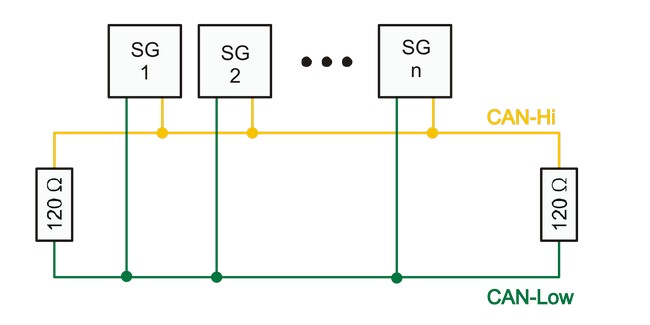
\includegraphics[width=0.8\textwidth]{Esquema-bus-can}
 \caption{Estructura de un bus \acro{can}}
 \label{fig:Esquema-bus-can}
 \end{figure}

La transmissió del senyal es realitza mitjançant comunicació per voltatge diferencial; és a dir, el senyal útil es determina a partir de la diferència de voltatge entre les 
línies \acro{can} \textit{High} i \acro{can} \textit{Low}. Aquest mètode no depèn d'un node de referència i té com a objectiu fer la comunicació resistent a interferències electromagnètiques presents en 
l'entorn del vehicle. Si un senyal extern afecta el bus, aquest impactarà amb pràcticament la mateixa intensitat en tots dos cables, mantenint inalterada la diferència de 
potencial i, per tant, la integritat del senyal. L'ús de cables trenats contribueix a aquest efecte, ja que millora l'equilibri elèctric i assegura que les pertorbacions 
afectin per igual ambdues línies.

Els nivells de voltatge utilitzats són els següents:

\begin{itemize}
  \item \textbf{Bit 1 (recessiu)}: El \acro{can} \textit{High} i el \acro{can} \textit{Low} tenen tots dos un voltatge de 2,5 Volts, amb una diferència de 0 Volts entre ells.

  \item \textbf{Bit 0 (actiu)}: El \acro{can} \textit{High} té un voltatge de 3,75 Volts i el \acro{can} \textit{Low} de 1,25 Volts, generant una diferència de 2,5 Volts.
\end{itemize} 

Els nodes, per transmetre un 1, deixen la seva connexió al bus en alta impedància, és a dir, no forcen cap voltatge sobre el bus. Aquest és l'estat per defecte del bus, 
i per aquest motiu parlem de valor recessiu quan identifiquem un bit 1. En canvi, quan els nodes volen transmetre un 0, forcen un voltatge sobre el bus, i aquest estat es 
coneix com a actiu.

Gràcies a aquest disseny, el bus pot actuar amb una lògica \textit{wired-AND}. Això significa que, si tots els nodes volen transmetre un bit recessiu (1), el bus es manté en aquest 
estat. Però si algun node transmet un bit actiu (0), aquest preval i tot el bus passa a l'estat actiu. Aquesta lògica serà la responsable de l'arbitratge en el bus, com veurem 
més endavant en la capa d'enllaç.

Segons la normativa, la velocitat màxima de transmissió és d'1 Mbit/s. Tanmateix, aquesta velocitat es pot veure reduïda en funció de la longitud del bus i del retard de 
propagació del cable. Està establert per normativa que un bus que operi a 1 Mbit/s ha de tenir una longitud màxima inferior a 40 metres. Per a velocitats de transmissió 
més baixes, i per garantir una comunicació fiable, el retard màxim entre els dos punts més allunyats del bus ha de ser inferior a la durada d'un bit. Per tant, cal calcular 
la longitud màxima tenint en compte aquest factor.

Un detall rellevant és que la normativa no defineix un connector físic estàndard per a la connexió dels nodes al bus. Tot i que aquesta flexibilitat pot resultar útil en 
determinades aplicacions, també pot provocar problemes d'incompatibilitat entre dispositius. Actualment, molts fabricants han optat per utilitzar connectors DE-9
com el que podem apreciar a la següen figura \ref{fig:db9-connector}.

 \begin{figure}
 \centering
 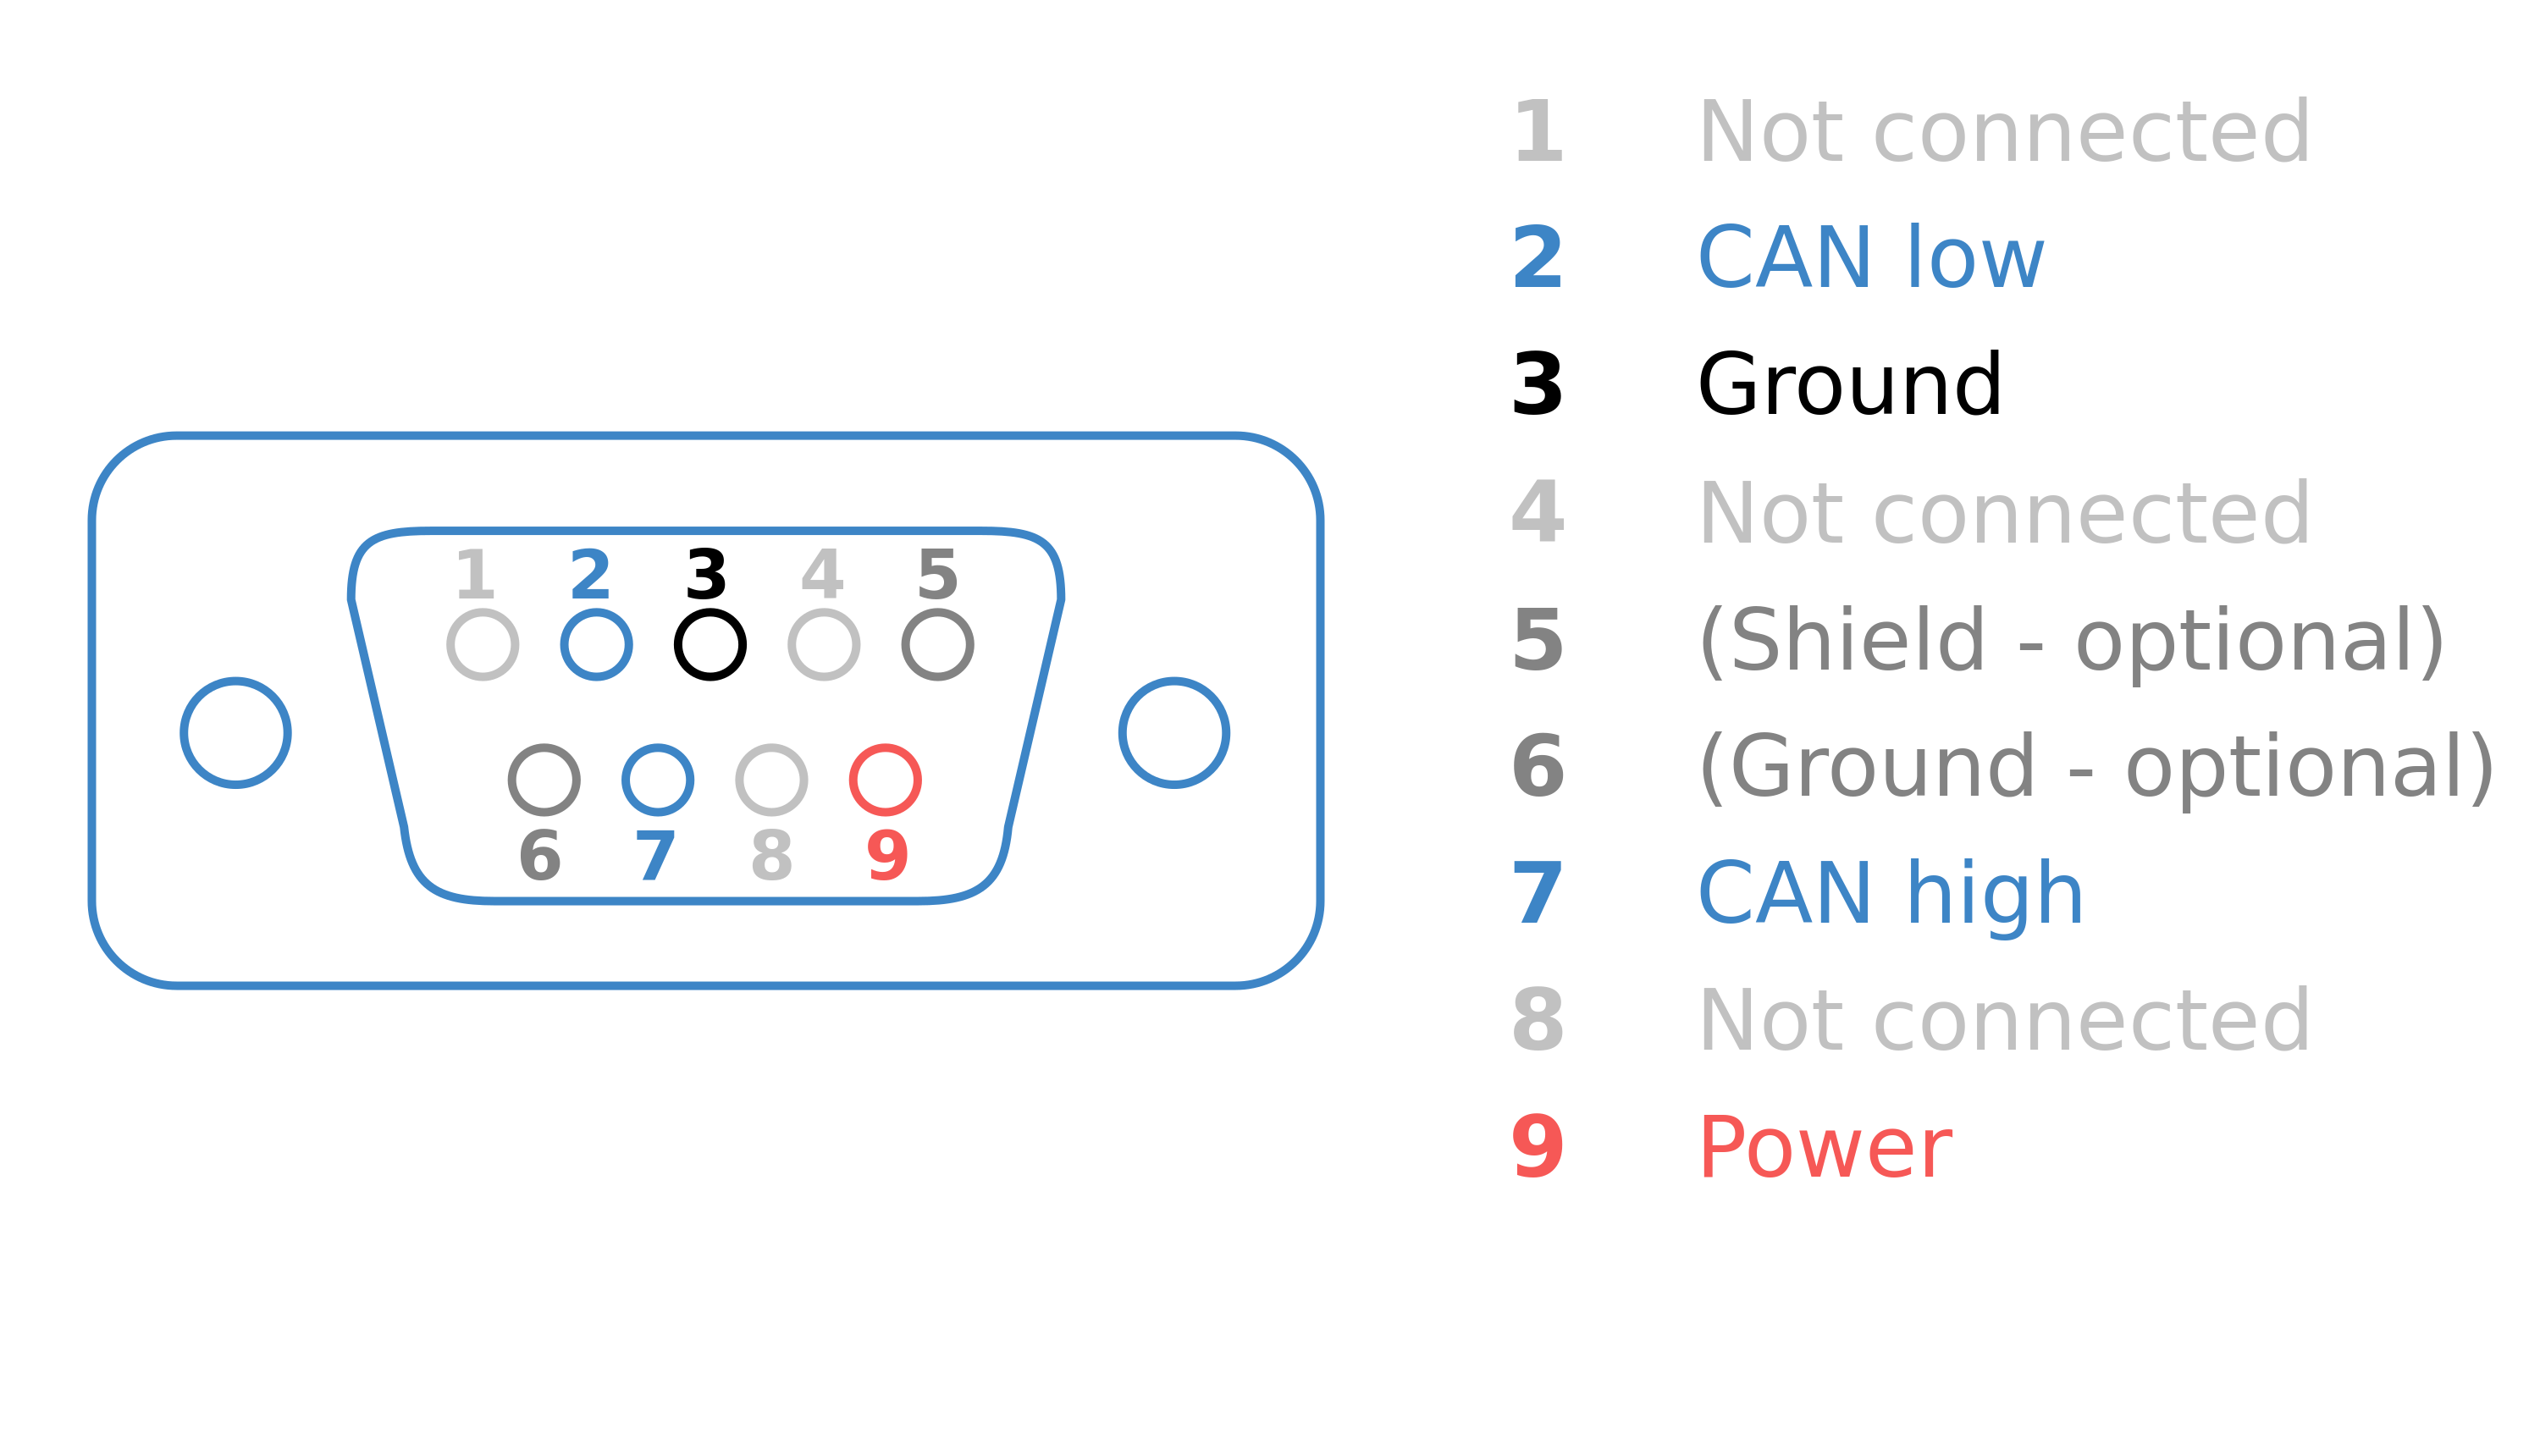
\includegraphics[width=0.8\textwidth]{db9-connector.png}
 \caption{Pinout del connector DE-9}
 \label{fig:db9-connector}
 \end{figure}

Per tant, tot node \acro{can} haurà d'incloure els següents elements: El microprocessador i el controlador, responsables de seguir la lògica del protocol (aquest últim genera els 
senyals lògics). El transceptor \acro{can}, encarregat de convertir els senyals lògics als nivells de voltatge utilitzats pel bus.

El transceptor consta d'un senyal TX i un RX connectats al controlador, a més dels senyals \acro{can} High i \acro{can} Low. RX sempre sondeja el bus i tradueix el seu senyal en un valor 
lògic, independentment de si es vol transmetre o no. TX tradueix els valors lògics que es volen enviar i els força sobre el bus. Per tant, si s'està transmetent, TX i RX 
indiquen el mateix valor en tot moment.

Tal com hem esmentat, per transmetre un 1, el transceptor no força cap senyal sobre el bus, i els seus transistors queden en alta impedància, de manera que no afecten el bus. 
El que manté el voltatge al bus és la seva connexió a una xarxa de polarització interna, similar a un \textit{pull-up/pull-down}. D'altra banda, el node ha d'incloure una resistència 
de 120 ohms curtcircuitant \acro{can} High i \acro{can} Low només si és un dels dos nodes terminals del bus. Si no és el cas, el node ha de quedar en alta impedància per no tenir cap efecte al valor 
resistiu del bus.

\subsection{Capa d'enllaç}

Aquesta normativa descriu les propietats del protocol \acro{can} a nivell de capa d'enllaç, a partir dels camps que componen les seves trames de missatge.

Es defineixen diversos tipus de trames \acro{can}. A continuació, s'enumeren amb una breu explicació dels seus camps principals. Més endavant, es detallaran les implicacions 
específiques de cadascun. Les imatges i referenecies d'aquest apartat provenen en part de \cite{andry_can_frame}

\subsubsection{Data Frame}

És l'únic tipus de trama que inclou un camp destinat a la transmissió de dades. Per tant, no es limita només a la gestió del canal de comunicació, sinó que permet enviar informació 
útil entre dispositius. En aquesta figura \ref{fig:can-frame} es pot visualitzar el seu format, a continuació s'expliquen els seus camps. 

 \begin{figure}
 \centering
 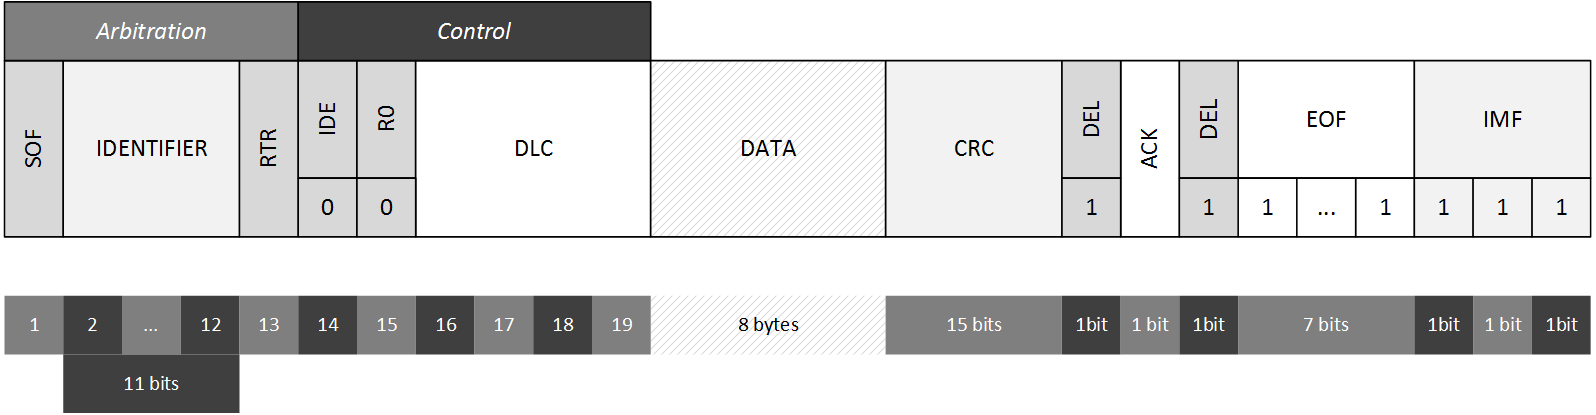
\includegraphics[width=0.8\textwidth]{can-frame.png}
 \caption{Format d'una trama de dades \acro{can} estàndard}
 \label{fig:can-frame}
 \end{figure}

\begin{itemize}
  \item \textbf{Start of Frame (SOF) (1 bit)}: Bit dominant (0) que marca l'inici del missatge.

  \item \textbf{Identifier (ID) (11 bits)}: Identificador únic que defineix el destinatari del missatge i la prioritat.
  
  \item \textbf{Remote Transmission Request (RTR) (1 bit)}: En una \textit{Data Frame}, aquest bit és dominant (0), indicant que es tracta d'un missatge amb dades reals.
  
  \item \textbf{Identifier Extension Bit (IDE) (1 bit)}: Indica si s'està utilitzant un identificador estès (29 bits). En el format estàndard, aquest bit val 0.
  
  \item \textbf{Reserved Bit (r0) (1 bit)}: Bit reservat per a futures ampliacions. Sempre dominant (0).
  
  \item \textbf{Data Length Code (DLC) (4 bits)}: Indica la quantitat de bytes de dades que conté el missatge (de 0 a 8).
  
  \item \textbf{Data Field (0-64 bits / 0-8 bytes)}: Conté les dades útils del missatge. La seva mida està determinada pel camp \acro{dlc}.
  
  \item \textbf{Cyclic Redundancy Check (CRC) (15 bits)}: Valor generat a partir dels bits que conté la trama fins a aquest punt, serveix per detectar errors en la transmissió.

  \item \textbf{CRC Delimiter (1 bit)}: Bit recessiu que separa el camp \acro{can} del camp \acro{ack}.
  
  \item \textbf{Acknowledgment (ACK) Slot (1 bit)}: Emès pel receptor. Si el missatge s'ha rebut correctament, aquest bit és dominant (0).
  
  \item \textbf{ACK Delimiter (1 bit)}: Bit recessiu que separa l'\acro{ack} del final del missatge.
    
  \item \textbf{End of Frame (EOF) (7 bits)}: Set bits recessius que indiquen el final de la trama.
  
  \item \textbf{Intermission Frame (IFS) (3 bits)}: Tres bits recessius que separen dues trames consecutives i permeten un breu estat d'inactivitat del bus.
\end{itemize} 

\subsubsection{Remote Frame}

Aquest tipus de trama serveix per so\l.licitar dades a un altre \acro{ecu} del bus, especificant-ne l'\acro{id}. En resposta, l'\acro{ecu} destinatària enviarà un \textit{Data Frame} 
amb les dades so\l.licitades. Té el mateix format que un \textit{Data Frame} amb les diferencies descrites a continuació.

\begin{itemize}
  \item \textbf{RTR}: Aquest bit és recessiu (1), indicant que es tracta d'una petició remota.

  \item \textbf{Data Field}: No existeix. Com que no es transmeten dades, aquest camp s'omet.
  
  \item \textbf{DLC}: Tot i no portar dades, aquest camp indica la longitud de les dades que es desitgen rebre.
\end{itemize} 

\subsubsection{Error Frame}

Les trames d'error són transmeses per qualsevol node (tant transmissor com receptor) que detecti un error durant la comunicació. La seva funció és informar la 
resta de nodes que la trama actual conté errors. A continuació se citen els camps d'un \textit{Error Frame}:

\begin{itemize}
  \item \textbf{Error Flags (6 bits)}: Indiquen l'estat del node que ha detectat l'error donant dues possibilitats

  \begin{itemize}
  \item \textbf{6 bits dominants (0)}: Representen un \textit{Active Error Frame}, emès per un node actiu. Aquest senyal interromp immediatament la comunicació.

  \item \textbf{6 bits recessius (1)}: Representen un \textit{Passive Error Frame}, emès per un node en estat passiu (amb un historial d'errors). No interromp la 
  transmissió, però informa de l'error.
  
  \end{itemize} 
  
  \item \textbf{Error Delimiter (8 bits)}: Sempre recessius (1). Marca el final de la trama d'error i permet que el bus es recuperi i torni a l'estat normal.
  
  \item \textbf{IFS (3 bits)}: Tres bits recessius que separen dues trames consecutives i permeten un breu estat d'inactivitat del bus.
\end{itemize} 

\subsubsection{Overload Frame}

És una trama especial que s'utilitza per demanar un petit retard abans de la següent transmissió. El seu format és idèntic al d'un \textit{Active Error Frame}. 
El seu objectiu és concedir temps addicional a un node per processar informació o gestionar una situació de sobrecàrrega temporal. Les \acro{ecu}s poden interpretar 
si es tracta d'un \textit{Overload Frame} o \textit{Active Error Frame} un altre segons el context, gràcies al moment i condicions en què es transmet.

\subsubsection{Identificació i trames expandides}

En qualsevol protocol de comunicació amb múltiples nodes és imprescindible assignar una identificació única a cadascun d'ells per garantir una comunicació ordenada. 
En el cas concret del bus \acro{can}, com que es tracta d'un bus de transmissió compartida on tots els missatges arriben a tots els nodes connectats, el sistema està dissenyat 
perquè cada \acro{ecu} ignori els missatges que no li van dirigits, basant-se en el camp d'identificador del missatge.

El camp d'identificador del protocol \acro{can} estàndard té una mida d'11 bits, fet que permet definir fins a 2048 identificadors únics. Aquesta quantitat és suficient per a 
la majoria d'aplicacions en el sector de l'automoció, on habitualment es treballa amb entre 40 i 70 \acro{ecu}s. No obstant això, en altres aplicacions aquesta capacitat pot 
resultar insuficient. Per aquest motiu, existeixen les trames esteses, que incorporen camps d'identificador de 29 bits.

Aquest és el principal factor diferenciador entre els protocols \acro{can} 2.0 A i \acro{can} 2.0 B. \acro{can} 2.0 A només admet trames estàndard amb 
identificadors d'11 bits. En canvi, el \acro{can} 2.0 B és més flexible, ja que admet tant trames estàndard com trames esteses amb identificadors de 29 bits.
Els nodes implementats amb \acro{can} 2.0 A no reconeixen les trames esteses i, segons l'especificació, les interpreten com a missatges erronis, generant una trama d'error en 
resposta. Això pot provocar problemes d'interoperabilitat en sistemes mixtos.

Per resoldre aquesta limitació, els nodes \acro{can} 2.0 B poden operar en dos modes:

\begin{itemize}
  \item \textbf{Mode actiu}: El node pot transmetre i rebre tant trames estàndard com esteses.

  \item \textbf{Mode passiu}: El node només transmet i accepta trames estàndard, però no genera errors si rep trames esteses. Aquesta funcionalitat permet que un 
  dispositiu \acro{can} 2.0 B pugui operar en entorns on hi hagi nodes \acro{can} 2.0 A, millorant la compatibilitat i l'estabilitat de la xarxa.
\end{itemize} 

Les trames esteses tenen un format diferent respecte a les trames estàndard, i aquesta diferència afecta exclusivament les trames de dades i les de so\l.licitud remota. 
En aquesta figura \ref{fig:can-frame-ext} podem apreciar el format d'una trama expandida. A continuació es descriuen les principals diferències en el format de les trames esteses. 

 \begin{figure}
 \centering
 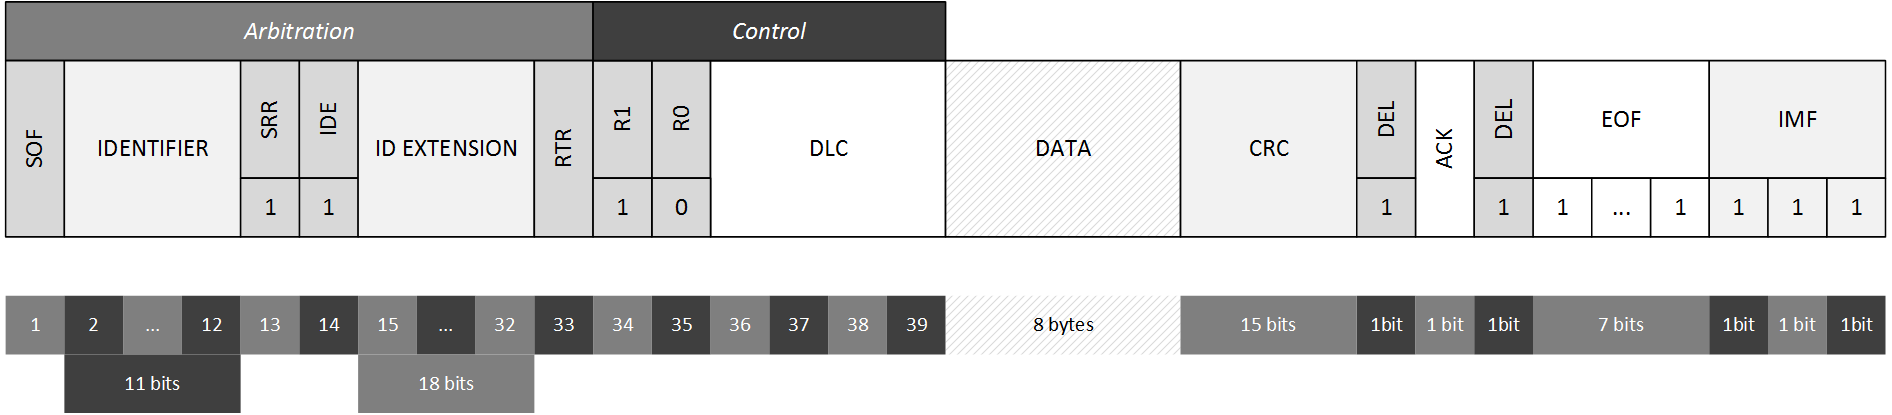
\includegraphics[width=0.8\textwidth]{can-frame-ext.png}
 \caption{Format d'una trama de dades \acro{can} expandides}
 \label{fig:can-frame-ext}
 \end{figure}

\begin{itemize}
  \item \textbf{Identifier A}: El camp d'identificador de 11 bits continua existint i ocupa la primera part de l'\acro{id}.

  \item \textbf{Substitute Remote Request (SRR)}: Aquest bit sempre té el valor recessiu (1). El seu propòsit és assegurar 
  que una trama de dades estàndard tingui prioritat si comparteix els mateixos 11 bits d'identificador.

  \item \textbf{IDE}: En les trames esteses, aquest camp val sempre un valor recessiu (1)

  \item \textbf{Identifier B}: Aquest camp completa el valor de l'identificador, afegint-hi els 18 bits addicionals per arribar als 29 bits totals.

  \item \textbf{RTR}: En les trames esteses, aquest camp apareix després dels 18 bits addicionals de l'identificador. 
  Igual que en les trames estàndard, indica si la trama és de dades o de so\l.licitud remota.

  \item \textbf{Reserved bit (r1)}: En comptes d'haver-hi únicament un bit reservat, hi ha aquest bit previ que ha de valdre un valor recessiu (1) previ a l'altre r0.

\end{itemize} 

\subsubsection{Prioritats}

A la secció dedicada a l'\acro{id}, s'ha destacat que aquest també determina la prioritat del missatge dins del bus \acro{can}. Aquesta funcionalitat 
es basa en la propietat \textit{wired-AND} del bus, on els bits dominants (0) sempre tenen prioritat sobre els bits recessius (1).

Quan dues \acro{ecu}s transmeten simultàniament, el procés d'arbitratge comença amb l'enviament de l'\acro{id} del missatge. Durant aquesta fase, el bus compara bit a bit 
el senyal de cada transmissor. Si una \acro{ecu} envia un bit recessiu (1) mentre una altra envia un bit dominant (0) en la mateixa posició, la primera detecta una 
discrepància (ja que el bus reflecteix el 0) i abandona la transmissió automàticament, sense generar errors. D'aquesta manera, l'\acro{ecu} amb l'\acro{id} numèricament més 
petit sempre obté accés al bus sense interrupcions.

Un altre criteri rellevant és el que s'aplica a les trames esteses, quan un \acro{id} estàndard i un d'estès coincideixen numèricament, la trama estàndard té prioritat, 
ja que el seu identificador (considerant en la seva forma completa) és més curt i, en la pràctica, equival a un valor numèric inferior.

Així doncs, els missatges amb \acro{id} més baix disposen de major prioritat en el bus \acro{can}. Per aquest motiu, l'assignació d'identificadors no és arbitrària, sinó que es 
dissenya en funció de la criticitat del sistema. Per exemple, sistemes crítics com el \acro{abs} reben \acro{id}s més baixos que sistemes menys prioritaris, 
com el control de les finestres del vehicle.

\subsubsection{Accés al medi}

En qualsevol protocol de comunicacions, és essencial implementar un mecanisme d'accés al medi que eviti transmissions simultànies i co\l.lisions.

En el cas del bus \acro{can}, no hi ha un controlador central que autoritzi la transmissió; en lloc d'això, els nodes actuen de manera descentralitzada. Abans de transmetre, 
cada node verifica l'estat del bus mitjançant el mecanisme \acro{csma/ca} (\textit{Carrier Sense Multiple Access with Collision Avoidance}): si detecta activitat, espera 
fins que el bus estigui lliure.

No obstant això, encara pot succeir que diversos nodes intentin transmetre exactament al mateix temps. En aquests casos, el protocol \acro{can} resol el conflicte mitjançant 
el sistema d'arbitratge per prioritat que hem explicat anteriorment. El node que hagi interromput la seva transmissió intentarà enviar just quan quedi el bus lliure.

Aquest mètode elimina la necessitat de mecanismes addicionals de gestió de co\l.lisions, com el backoff exponencial utilitzat en protocols com Ethernet. En \acro{can}, els 
missatges crítics, com una activació del \acro{abs}, no queden en espera per retards aleatoris, sinó que accedeixen al bus amb mínima latència, garantint una resposta ràpida 
i determinista. Aquesta eficiència el fa ideal per sistemes en temps real, on la priorització és clau.

\subsubsection{Bit timing i sincronització}

Tal com s'ha comentat anteriorment, el protocol \acro{can} opera sobre un bus asíncron, és a dir, no existeix cap senyal de rellotge compartit entre els nodes. Això obliga a implementar 
mecanismes de sincronització, perquè tots els nodes puguin interpretar correctament l'estat del bus en cada moment. És crucial remarcar que tots els nodes han de funcionar 
exactament a la mateixa velocitat de transmissió (baud rate), de manera que la durada d'un bit sigui igual per a tots. Part de la informació d'aquest apartat prove de \cite{getbyte_can_timing}.

La sincronització d'un node receptor comença amb el \acro{sof}. Quan el node detecta una transició en el senyal del bus, interpreta aquest canvi com l'inici d'un nou bit i 
sincronitza el seu temporitzador amb aquest punt. Aquesta primera sincronització s'anomena hard synchronization, ja que marca clarament l'inici d'una nova trama.

Tanmateix, durant la transmissió poden aparèixer desincronitzacions provocades per diversos factors, com ara les característiques físiques del cablejat, retards de propagació, interferències 
electromagnètiques o desajustos entre els rellotges interns dels nodes. A causa d'aquests factors, es podrien produir derives temporals que afectin la lectura correcta dels bits.

Per tal de corregir aquests desfasaments i mantenir la precisió temporal durant tota la comunicació, el protocol \acro{can} incorpora un mecanisme anomenat soft synchronization. Aquest mecanisme 
consisteix a ajustar novament la sincronització del node receptor cada vegada que es detecta una nova transició en el senyal. Així, el temporitzador intern es recalibra prenent com a nova 
referència el moment exacte d'aquesta transició, compensant possibles desviacions entre rellotges.

\begin{figure}
  \centering
  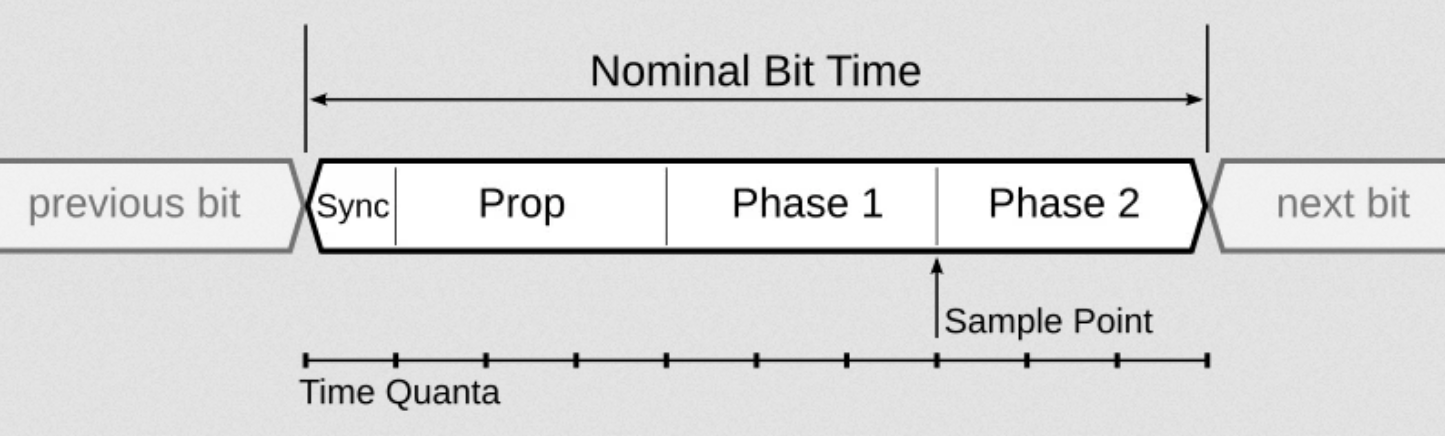
\includegraphics[width=0.8\textwidth]{CAN-bit-timing.png}
  \caption{Segments en el que es divideix un bit \acro{can}}
  \label{fig:CAN-bit-timing}
  \end{figure}

Per tal de controlar amb precisió el moment en què es pren la mostra d'un bit, els nodes divideixen la durada d'un bit en quatre segments, com els que veiem a aquesta figura 
\ref{fig:CAN-bit-timing}, cadascun dels quals ocupa un nombre enter d'unitats de temps anomenades \textit{Time Quanta} (\acro{tq}). El \textit{Time Quanta} 
és la unitat mínima de temps que pot mesurar el controlador \acro{can}.

\begin{itemize}
  \item \textbf{Sync Segment}: Té una durada fixa d'1 \acro{tq}. Serveix per indicar l'inici del bit. Si es detecta una transició en el senyal del bus, els nodes sincronitzen els seus rellotges a aquest punt.

  \item \textbf{Propagation Segment}: Serveix per compensar els retards físics en la propagació del senyal a través del bus. La seva durada es configura en funció de les característiques físiques del sistema. 
  Pot durar entre 1 i 8 \acro{tq}.

  \item \textbf{Phase Segment 1 i 2}: Aquests segments permeten ajustar el punt de mostreig del bit. Si es detecta que la transició del senyal s'ha produït abans del previst, es pot allargar el 
  Phase Segment 1 o escurçar el Phase Segment 2 per compensar la diferència. Cadascun d'aquests segments pot tenir una durada configurable entre 1 i 8 \acro{tq}. El punt de mostreig 
  es troba entre el final del Phase Segment 1 i l'inici del Phase Segment 2.
\end{itemize} 

\subsubsection{Bit stuffing}

Tal com s'ha mencionat, els nodes han de mantenir una sincronització constant amb el senyal del bus per poder interpretar correctament els missatges. Per aquest motiu, 
si un mateix valor de bit (0 o 1) es repeteix massa vegades consecutives durant la transmissió d'un missatge, els nodes podrien perdre la sincronització, fet que pot 
provocar errors en la recepció.

Per evitar aquesta situació, el protocol \acro{can} incorpora una mesura coneguda com a bit \textit{stuffing}. Aquesta tècnica consisteix a inserir un bit addicional de valor 
contrari cada vegada que s'han transmès cinc bits consecutius iguals. Per exemple, si s'han enviat cinc bits (1) seguits, es co\l.loca automàticament un bit (0) 
a continuació. Aquest bit inserit no conté informació útil, sinó que simplement garanteix que hi hagi prou transicions de nivell per mantenir la sincronització 
dels nodes receptors.

Els receptors, coneixedors d'aquesta norma, eliminen automàticament aquests bits de \textit{stuffing} durant la descomposició del missatge per recuperar les dades originals. 
No obstant això, un dels reptes d'aquesta tècnica és que un error de transmissió pot fer que un bit de dades es confongui amb un bit de \textit{stuffing} o viceversa, cosa que 
pot provocar que el receptor no detecti a temps l'error o que el detecti de forma incorrecta.

És important destacar que els bits de \textit{stuffing} només s'apliquen entre els camps \acro{sof} i \acro{can} incloent els dos. Els camps posteriors, com el 
\acro{can} \textit{delimiter} i l'\acro{ack}, tenen longituds fixes i valors predefinits, i per tant no estan subjectes a bit \textit{stuffing}. Pel càlcul del \acro{can} els bits 
de \textit{stuffing} tampoc tenen cap implicació.

\subsubsection{ACK i CRC}

A continuació es tracten, els camps de les trames \acro{can} ideats per evitar errors en els missatges. Són mecanismes fonamentals per assegurar la integritat i fiabilitat 
de la comunicació.

Un d'aquests mecanismes és el \acro{can}, un valor numèric de 15 bits calculat a partir del contingut del missatge previ al propi \acro{can}.  
Quan un node rep el missatge, recalcula el \acro{can} i el compara amb el rebut. Si coincideixen, es considera que la transmissió ha estat correcta. 
El càlcul es basa en aaquest polinomi estàndard:

\( x^{15} + x^{14} + x^{10} + x^{8} + x^{7} + x^{4} + x^{3} + x^{0} \)

Un altre mecanisme clau és el bit d'\acro{ack}. El transmissor envia aquest bit en estat recessiu, i si un receptor valida correctament el missatge 
(verificant el \acro{can}), escriu un bit dominant en el bus durant aquest temps. El transmissor llegeix el bus i, si detecta el bit dominant, interpreta 
que el missatge ha arribat correctament a almenys un node. Si cap node escriu el bit dominant, el transmissor interpreta que la transmissió ha fallat 
i reenviarà automàticament la trama.

\subsubsection{Gestió d'errors}

La xarxa \acro{can}, com s'ha vits, disposa de diversos mecanismes per detectar i gestionar errors. Quan algun d'aquests mecanismes falla, es genera una trama d'error per 
notificar la incidència i interrompre la transmissió.

Els 5 mecanismes de detecció d'errors que ja s'han tractat són:

\begin{itemize}
  \item \textbf{Bit monitoring}: El node transmissor compara el nivell del bus amb el bit que envia. Si detecta una discrepància, es genera una trama d'error. 
  Aquest control no s'aplica durant l'arbitratge, ja que és normal que un node cedeixi davant un \acro{id} més prioritari.

  \item \textbf{Bit stuffing}: Si un receptor detecta sis bits iguals seguits entre el \acro{sof} i el \acro{crc}, genera una trama d'error.

  \item \textbf{CRC}: Si el \acro{crc} rebut no coincideix amb el recalculat pel node receptor, es considera que el missatge està corromput i es genera una trama d'error.

  \item \textbf{ACK}: Si el transmissor no rep confirmació (bit dominant) durant la finestra d'\acro{ack}, entén que cap node ha rebut el missatge 
  correctament i genera una trama d'error.

  \item \textbf{Errors de format}: Si algun camp amb valor esperat (com el delimitador del \acro{crc}) no compleix la norma, per exemple, si apareix 
  un bit dominant on hauria d'haver-hi un recessiu, també es genera una trama d'error.

\end{itemize} 

Tant els nodes receptors com els transmissors poden generar trames d'error per notificar problemes en la comunicació. Aquestes trames com s'ha vist contenen 
sis bits dominants consecutius i interrompen la transmissió. En detectar aquesta situació, la resta de nodes també generen trames d'error, degut a que es 
detecta com un error de \textit{bit stuffing}, cosa que pot provocar una seqüència de fins a 12 bits dominants superposats com es pot apreciar a aquetsa figura \ref{fig:CAN-bus-error}:

 \begin{figure}
 \centering
 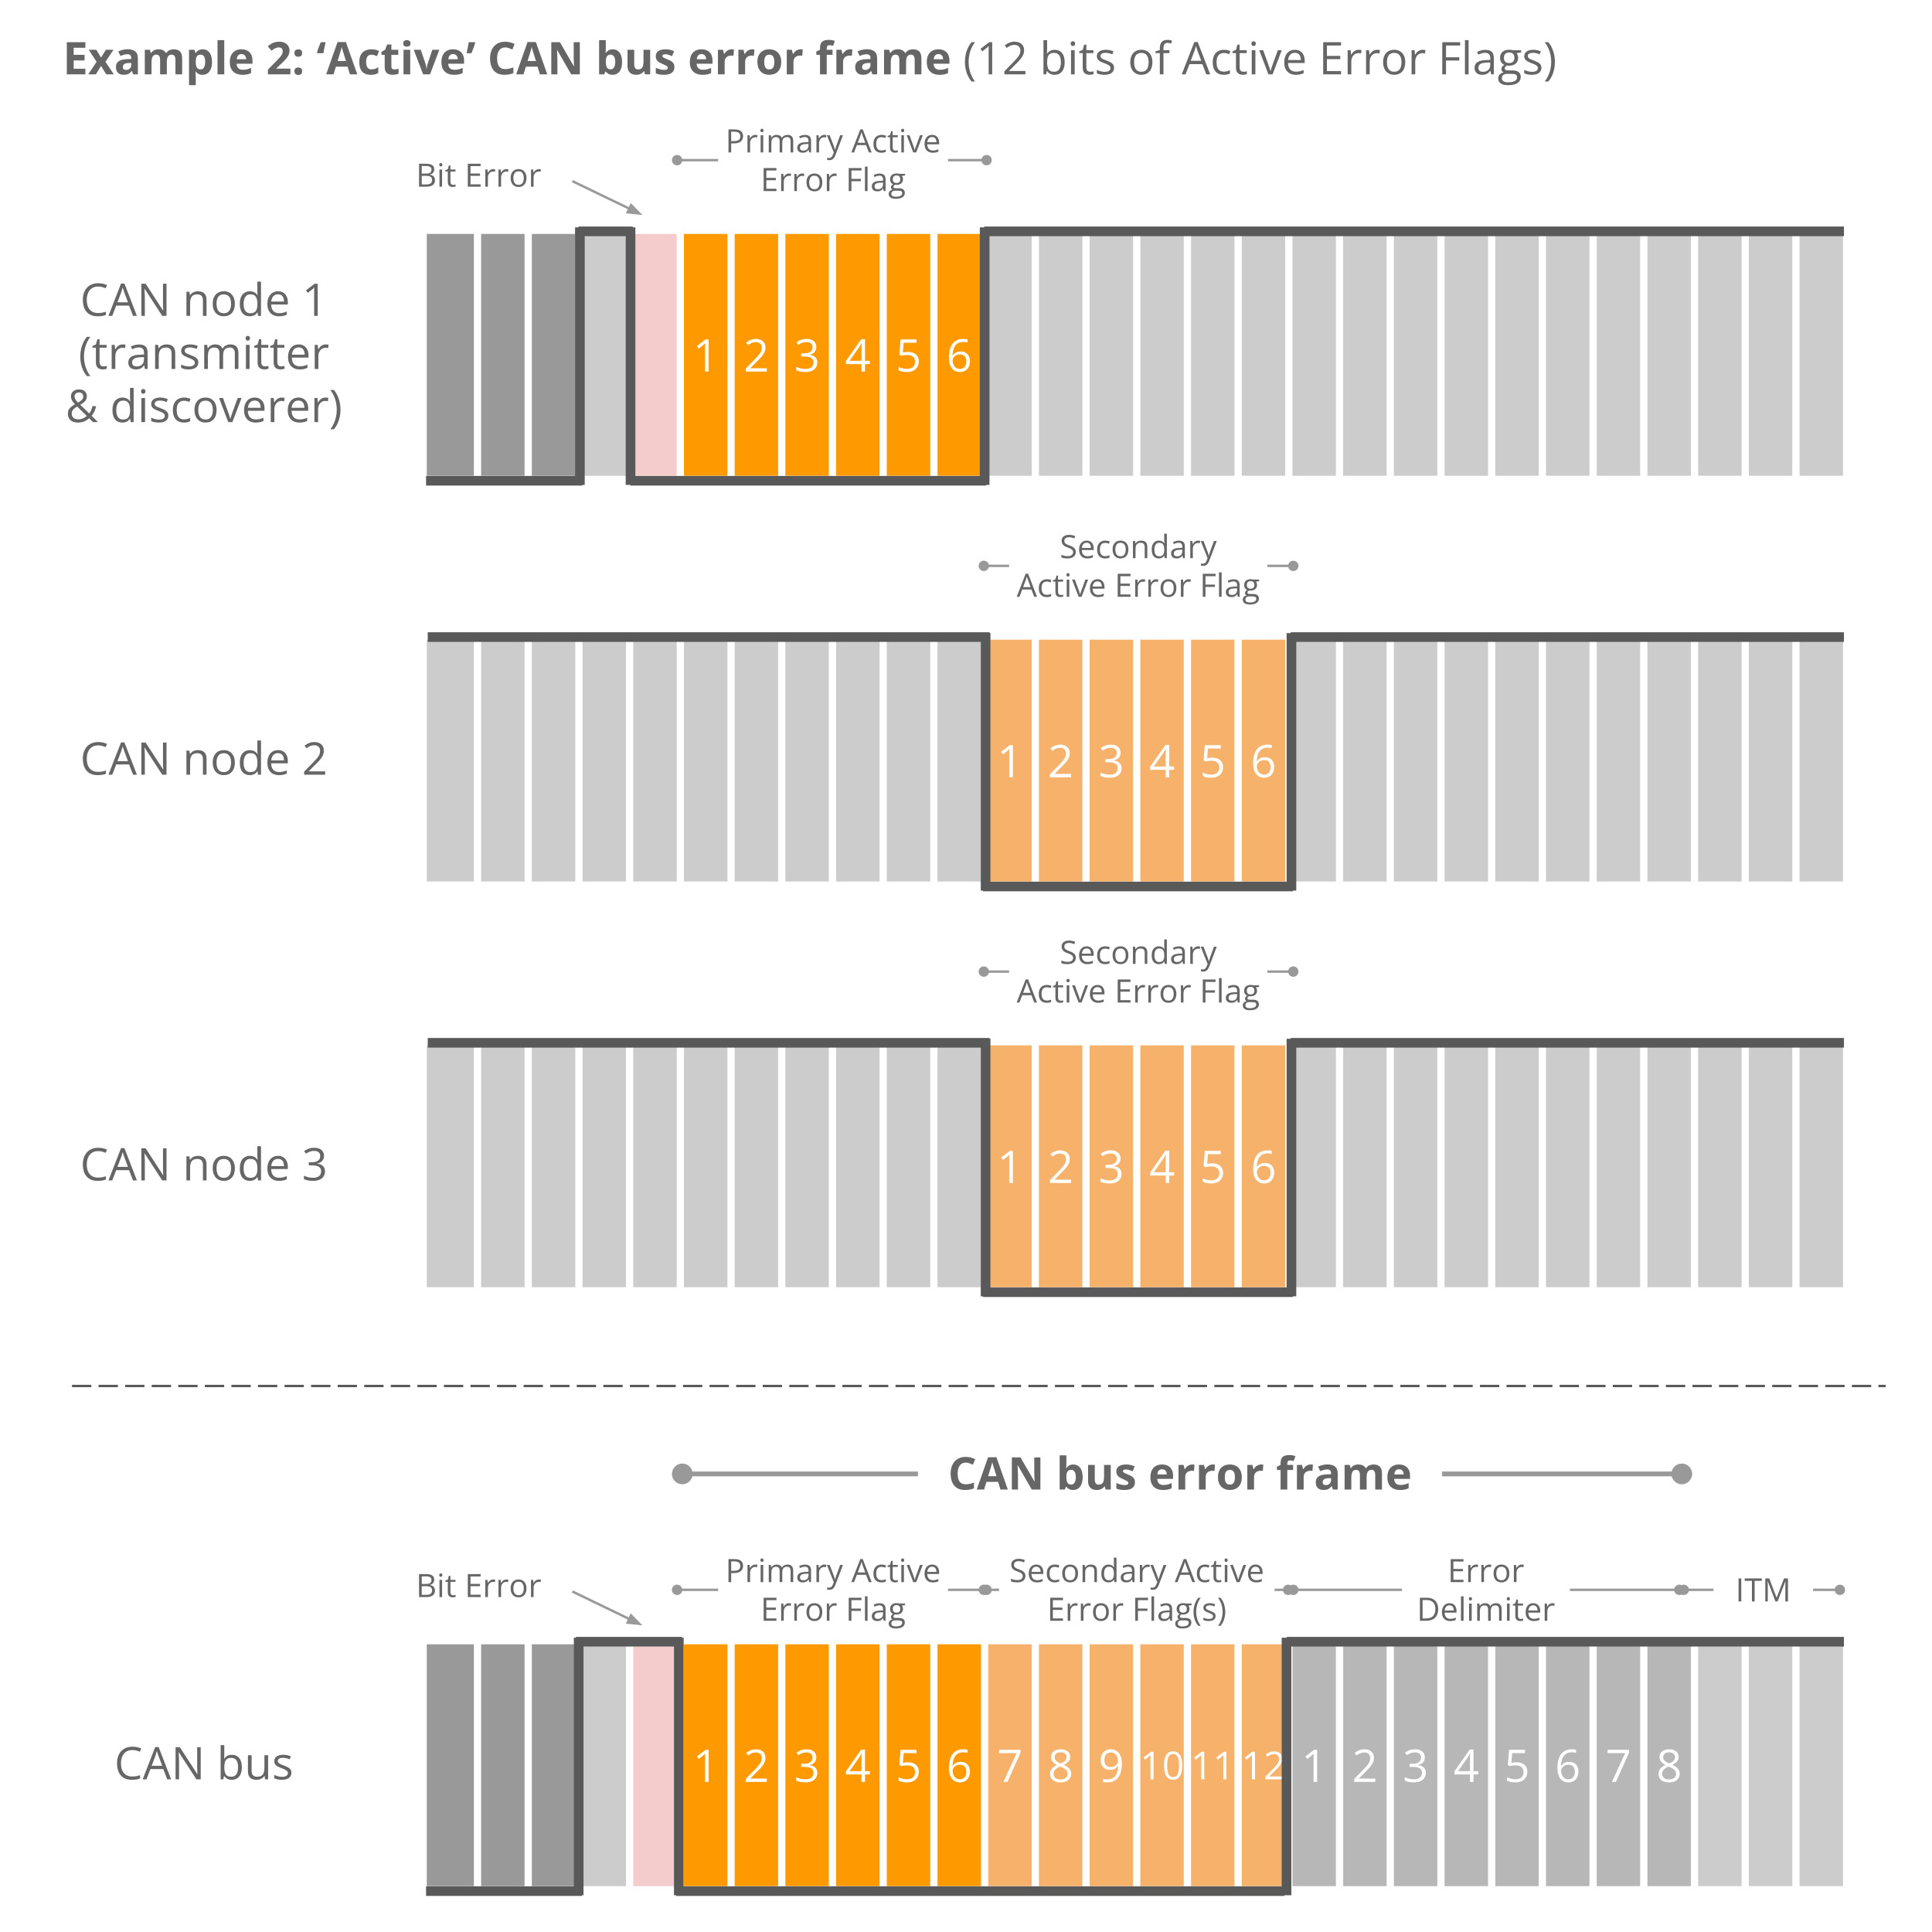
\includegraphics[width=0.8\textwidth]{CAN-bus-error.jpg}
 \caption{Superposició de dues trames d'error}
 \label{fig:CAN-bus-error}
 \end{figure}

 Quan es detecta un error, tots els nodes descarten el missatge i esperen fins que el bus torna a estar disponible per reprendre la comunicació. 
 El node que havia iniciat la transmissió torna a intentar enviar el missatge automàticament.

 Per gestionar els errors de manera eficient, cada node \acro{can} disposa de dos comptadors: un per a la recepció (\acro{rec}) i un per a la transmissió (\acro{tec}). 
 Quan es detecta un error, el transmissor incrementa el \acro{tec} en 8, mentre que els receptors incrementen el \acro{rec} en 1, excepte el node que ha detectat l'error, 
 que l'incrementa en 8. En canvi, si un missatge es transmet o rep correctament, el comptador corresponent es redueix en 1. Aquest sistema permet identificar 
 i penalitzar els nodes que generen més errors, contribuint així a mantenir la fiabilitat de la xarxa.

Els nodes \acro{can} poden estar en diferents estats operatius segons els seus comptadors d'error:

\begin{itemize}
  \item \textbf{Error Active}: És l'estat inicial de tots els nodes. Poden generar \textit{Active Error Frames} que interrompen la comunicació. Per mantenir-se en aquest 
  estat, tant el comptador de transmissió (\acro{tec}) com el de recepció (\acro{rec}) han d'estar per sota de 128.

  \item \textbf{Error Passive}: Quan qualsevol dels dos comptadors arriba a 128, el node entra en aquest estat. Només pot emetre 
  \textit{Passive Error Frames}, que no afecten la recepció dels altres nodes. A més, si vol tornar a transmetre, ha d'esperar un temps addicional de 8 bits 
  anomenat \textit{Suspend Transmission Time}, fet que li dóna menor prioritat al bus.

  \item \textbf{Bus Off}: Si el \acro{tec} arriba a 256, el node passa a l'estat \textit{Bus Off}, quedant totalment aïllat de la comunicació. No pot transmetre ni rebre 
  fins que es reinicia el node.
\end{itemize} 

Finalment, cal diferenciar entre \textit{Active Error Frame} i \textit{Overload Frame}. Un \textit{Active Error Frame} s'envia per interrompre la transmissió d'un missatge erroni.
Un \textit{Overload Frame} es genera entre trames per indicar que un node necessita més temps abans de continuar la comunicació. Tot i tenir el mateix format 
els nodes poden distingir-les i reaccionar adequadament.

\subsection{Altres version del protocol CAN}

La normativa ISO 11898 inclou diverses parts que defineixen diferents variants del protocol \acro{can}, adaptades a necessitats específiques.

Una d'aquestes és la ISO 11898-3, coneguda com a \textit{Low-Speed} \acro{can}. A diferència del \textit{High-Speed } \acro{can}, definit a la 
ISO 11898-2, aquesta variant està dissenyada per a aplicacions on la tolerància a fallades és essencial. Opera a velocitats més baixes, 
generalment entre 40 kbit/s i 125 kbit/s, i sovint s'utilitza en sistemes secundaris de vehicles, com alçavidres o controls de portes.

A més, la norma ISO 11898 inclou altres parts que recullen variants especialitzades del protocol, amb un abast més limitat i menys 
rellevància en contextos generals.

També és important destacar que el protocol \acro{can} continua evolucionant per respondre a les noves exigències dels sistemes electrònics. 
Aquesta evolució ha donat lloc a dues versions avançades del protocol:

\begin{itemize}
  \item \textbf{CAN FD}: Desenvolupat per Bosch el 2012, representa una millora substancial respecte al \acro{can} 2.0. Augmenta la capacitat de dades 
  per trama de 8 bytes a 64 bytes i permet velocitats de transmissió de fins a 5-8 Mb/s durant la fase de dades, mentre que la fase d'arbitratge 
  es manté a 1 Mb/s.
 
  Va ser incorporat a la norma ISO 11898-1 l'any 2015 i a la ISO 11898-2 el 2016, per donar suport a les noves característiques de velocitat i capacitat. 
  Malgrat això, encara no ha estat implementat dins de l'estàndard \acro{obd-ii}.
  
  \item \textbf{CAN XL}: Presentada el 2020, és l'evolució més recent del protocol. Amplia la capacitat de dades fins a 2048 bytes per trama i 
  pot assolir velocitats de transmissió de fins a 10 Mbps o més. Aquesta versió encara no forma part oficialment de la norma ISO 11898. Per més informació consultar \cite{can_cia_xl}.
\end{itemize} 

\section{Aplicació de CAN sobre sistemes de diagnosis}

Un cop entès el funcionament del protocol \acro{can}, és moment d'analitzar com s'aplica als sistemes de diagnosi a bord dels vehicles. 
L'estàndard que regula aquesta aplicació és la ISO 15765, que defineix tant les restriccions aplicades al protocol \acro{can} com la implementació 
de capes superiors per permetre la transmissió estructurada de missatges de diagnosi.

\subsection{Restriccions a la capa física i a la capa d'enllaç}

La norma ISO 15765-4 estableix limitacions específiques per a l'ús de \acro{can} en entorns de diagnosi vehicular. A la capa física, es fixen dues velocitats estàndard 
de transmissió:

\begin{itemize}
  \item 500 kbit/s per a vehicles lleugers
  
  \item 250 kbit/s per a vehicles pesats
\end{itemize} 

Aquesta uniformització facilita la compatibilitat entre fabricants i equips de diagnosi.

Pel que fa a la capa d'enllaç, es limita l'ús del protocol a \acro{can} 2.0B, amb trames de dades de màxim 8 bytes. A més, es prohibeix explícitament l'ús de \textit{Remote Frames}, 
ja que els protocols de diagnosi com \acro{obd-ii} es basen en un model de petició-resposta en què la informació s'inclou completament dins la pròpia trama, fent innecessàries 
les peticions separades de dades.

En el cas dels vehicles lleugers amb \acro{obd-ii}, s'utilitzen identificadors de 11 bits, i es reserven alguns \acro{id} concrets per a funcions específiques de diagnosi, com ara:

\begin{itemize}
  \item \textbf{0x7DF}: Per a missatges de broadcast
  
  \item \textbf{0x7E8 a 0x7EF}: Per a respostes dels diferents mòduls de control del vehicle
\end{itemize} 

Aquestes assignacions es detallen més endavant en el desenvolupament del protocol dins el context \acro{obd-ii}.

\subsection{Capa de xarxa i capa de transport}

Per gestionar missatges amb trames que superen els 8 bytes de camp de dades, es va desenvolupar un protocol de capa superior conegut com a ISO-TP recollit a 
la normativa ISO 15765-2. Per complementar la informació i alguna imatge s'ha consultat \cite{wikipedia_isotp} i \cite{emotive_isotp}. Aquest protocol permet la transmissió de missatges de fins a 
4095 bytes mitjançant segmentació, control de flux i reassemblatge. Per fer-ho, utilitza el camp de dades del protocol \acro{can}, definint quatre tipus de trames diferents, 
es poden apreciar en aquesta figura \ref{fig:iso-tp}.

 \begin{figure}
 \centering
 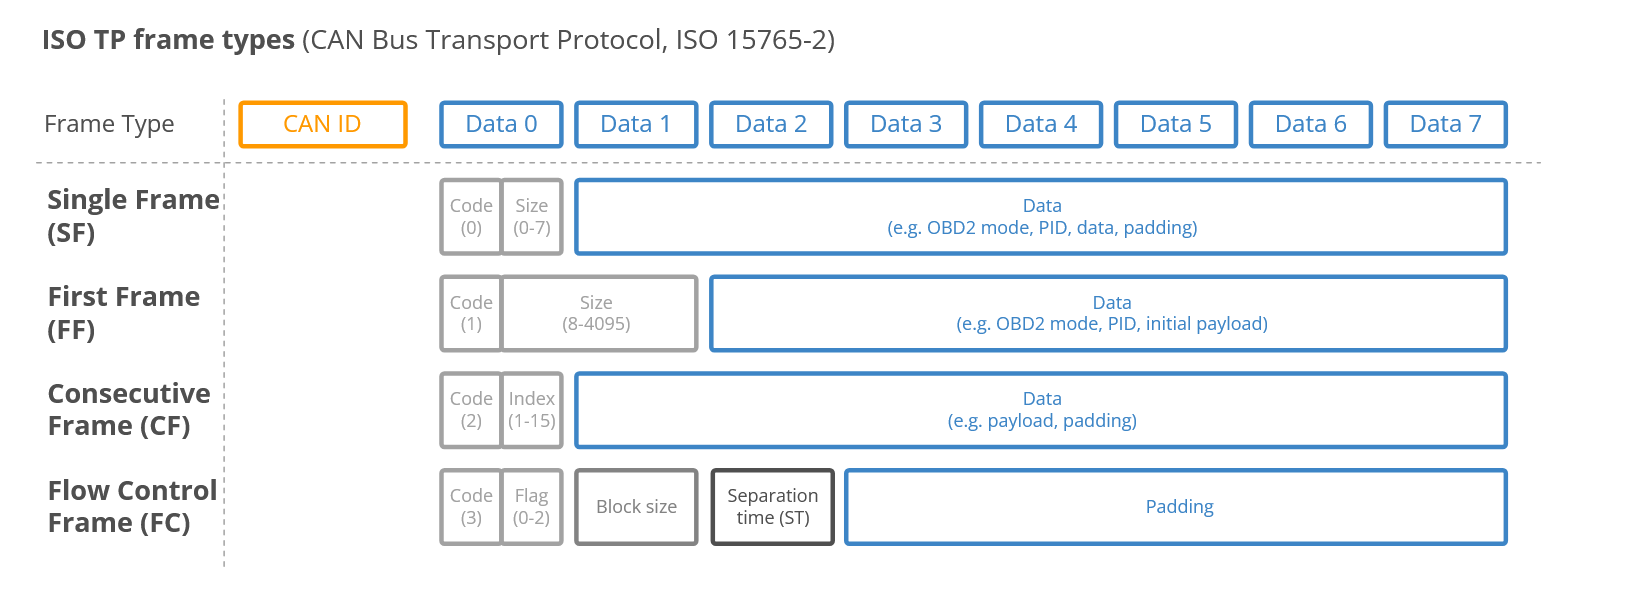
\includegraphics[width=0.8\textwidth]{ISO-TP-frame.png}
 \caption{Format de les trames utilitzades al protocol ISO-TP}
 \label{fig:iso-tp}
 \end{figure}

\subsubsection{Single Frame}

S'utilitza quan el missatge cap completament en 7 bytes. En aquest cas, no és necessària la segmentació.

\begin{itemize}
  \item \textbf{Code}: Ocupa el primer nibble del primer byte. Indica el tipus de trama; per a un \textit{Single Frame} val 0.
  
  \item \textbf{Size}: Ocupa el segon nibble del primer byte. Indica la mida del missatge en bytes útils.
  
  \item \textbf{Data}: Conté el contingut del missatge. Tot i que aquest pot ocupar menys de 7 bytes, el camp s'omple fins als 7 bytes mitjançant \textit{padding}.
\end{itemize} 

\subsubsection{First Frame}

S'utilitza per iniciar la transmissió d'un missatge que no cap en una sola trama.

\begin{itemize}
  \item \textbf{Code}: Primer nibble del primer byte, amb valor 1 per indicar \textit{First Frame}.
  
  \item \textbf{Size}: Format per la combinació del segon nibble del primer byte i tot el segon byte. Indica la mida total del missatge.
  
  \item \textbf{Data}: Conté els primers bytes del missatge.
\end{itemize} 

\subsubsection{Consecutive Frame}

S'utilitza per continuar la transmissió d'un missatge iniciat amb una \textit{First Frame}.

\begin{itemize}
  \item \textbf{Code}: Primer nibble del primer byte, amb valor 2.
  
  \item \textbf{Index}: Segon nibble del primer byte. Indica l'índex de la seqüència (de 1 a 15). Si multipliquem veiem que amb 15 missatges no es 
  suficient per arribar a la mida maxima de 4095, aixo es perque cada cop que s'arriba a 15 el valor es reinicia a 0. 
  
  \item \textbf{Data}: Conté una porció del missatge original, continuant des d'on es va deixar.
\end{itemize} 

\subsubsection{Flow Control}

S'utilitza per gestionar el flux de trames en una comunicació segmentada, enviant instruccions de control al transmissor del missatge segmentat.

\begin{itemize}
  \item \textbf{Code}: Primer nibble del primer byte, amb valor 3.
  
  \item \textbf{Flag}: Segon nibble del primer byte. Indica l'estat de control del flux. Hi ha 3 posibles valors: 
  \begin{itemize}
    \item \textbf{Continue To Send (0)}: El receptor está disponible per rebre més trames (\textit{Consecutive Frames}).
  
    \item \textbf{Wait (1)}: El receptor no esta preparat per rebre més dades, el transmisor ha d'esperar. Per continuar s'enviará un altre \textit{Flow Control}.
  
    \item \textbf{Overflow (2)}: El receptor no pot processar més dades, la transmissió s'ha de cancelar.
  \end{itemize} 
  
  \item \textbf{Block Size}: Indica el nombre màxim de \textit{Consecutive Frames} que es poden enviar abans de requerir una nova \textit{Flow Control}.
  
  \item \textbf{Separation Time}: Indica el temps mínim que ha de passar entre l'enviament de dues \textit{Consecutive Frames}.
  
  \item \textbf{Padding}: S'utilitza per omplir els bytes restants.
\end{itemize} 

En aquesta figura \ref{fig:ISOTP-Sample}, un node transmet les dades segmentades, mentre que l'altre regula el flux mitjançant trames \textit{Flow Control}. En aquest exemple, 
després d'enviar un \textit{First Frame}, el receptor respon amb una trama \textit{Flow Control} indicant que pot continuar rebent dades. En aquesta resposta, 
el segon nibble del primer byte és 0 (\textit{Continue To Send}), es permeten fins a 3 trames consecutives abans de demanar un nou control, i 
s'especifica un retard mínim de 10 ms entre missatges.

 \begin{figure}
 \centering
 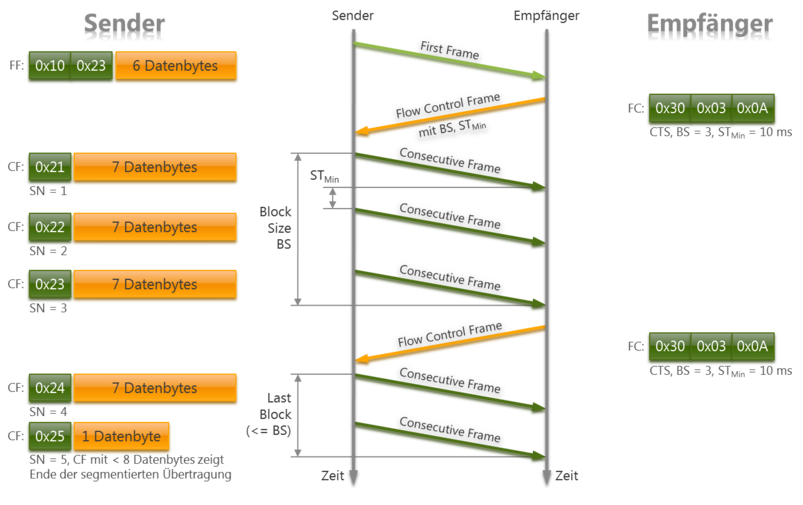
\includegraphics[width=0.8\textwidth]{ISOTP-Sample.png}
 \caption{Exemple de comunicació ISO-TP}
 \label{fig:ISOTP-Sample}
 \end{figure}

Com s'ha vist ISO-TP implementa funcionalitats típiques de la capa de transport del model \acro{osi}, com la gestió de fragments i el control de flux, assegurant 
una transmissió fiable i ordenada. Tot i això, sovint també es classifica com a protocol de xarxa, fet que pot portar a confusió, ja que no gestiona 
l'adreçament ni l'encaminament entre nodes, aquesta classificació és més un conveni que una classificació significativa. 

\section{OBD-II}

l'\acro{obd-ii} no és més que la capa d'aplicació que recull les dades del bus per mostrar-les a través del port \acro{obd-ii}.
Aquesta capa interpreta les dades provinents de les \acro{ecu}s, i permet l'accés a informació com ara codis d'error, paràmetres de funcionament del motor, 
emissions, velocitat, temperatura, entre d'altres.

Aquest protocol prové del seu predecessor, l'\acro{obd} (\textit{On-Board Diagnostics}), que va ser desenvolupat a finals dels anys 80 amb 
l'objectiu principal de monitorar les emissions contaminants dels vehicles. L'any 1996 es va introduir l'\acro{obd-ii}, la seva evolució, que va 
esdevenir obligatori als Estats Units per a tots els vehicles de nova fabricació i posterorment a la resta de territoris.


\subsection{Connector}

El connector \acro{obd-ii}, definit per la normativa SAE J1962, és l'estàndard emprat per a la diagnosi a bord dels vehicles. Consta de 16 pins, tot i que habitualment 
només se n'utilitzen alguns. En aquesta figura \ref{fig:OBD2-connector} podem apreciar el pinout del connector.

 \begin{figure}
 \centering
 \includegraphics[width=0.8\textwidth]{OBD2-connector.png}
 \caption{Pinout del connector \acro{obd-ii}}
 \label{fig:OBD2-connector}
 \end{figure}

Aquest connector admet diversos protocols de comunicació, com SAE J1850, ISO 9141 o el propi protocol \acro{can}. No obstant això, només un d'aquests protocols estarà actiu 
segons el sistema electrònic del vehicle. Aquesta versatilitat explica la presència de múltiples pins que poden quedar inactius en determinats casos.

Un dels pins més rellevants és el pin 16, destinat a l'alimentació elèctrica. Aquest subministra tensió directa de la bateria del vehicle, i és aquí on es diferencien 
les dues variants del connector:

\begin{itemize}
  \item \textbf{Tipus A}: Subministra 12 volts, habitual en vehicles lleugers.
  
  \item \textbf{Tipus B}: Subministra 24 volts, habitual en vehicles pesants.
\end{itemize} 

Finalment, per garantir una comunicació segura i estable, la normativa especifica que el cable del connector mascle no pot superar els 5 metres de longitud.

\subsection{Codis de errors (DTCs)}

A més de gestionar-ne el funcionament, les \acro{ecu}s poden estar programades per detectar condicions anòmales i, si escau, registrar errors mitjançant codis de 
diagnosi coneguts com a \acro{dtc}s (\textit{Diagnostic Trouble Codes}). Per exemple, si un sensor de temperatura proporciona valors fora del rang esperat o deixa de respondre, 
la \acro{ecu} responsable aplica una lògica de validació. Si es confirma l'anomalia, s'enregistra el codi \acro{dtc} corresponent a la seva memòria.

Quan l'error es considera rellevant o crític (per exemple, si afecta les emissions, la seguretat o pot causar danys mecànics), la \acro{ecu} que el detecta pot 
comunicar-ho a altres \acro{ecu}s a través del bus \acro{can}, especialment a la \acro{ecu} del motor, que normalment coordina accions globals. Aquest missatge no és un \acro{dtc}, 
sinó una notificació interna que pot desencadenar accions com ara limitar la potència del motor o activar el testimoni \acro{mil} (\textit{Malfunction Indicator Lamp}) 
al quadre d'instruments.

Els codis \acro{dtc} poden ser estàndard, comuns a tots els vehicles \acro{obd-ii}, o específics del fabricant, que ofereixen informació addicional segons la marca i model del vehicle.
Tot i aixo, \acro{dtc}s tenen un format estàndard de 5 caràcters alfanumèrics, que permet identificar de manera estructurada el tipus d'error detectat:

\begin{itemize}
  \item \textbf{1r caràcter}: Indica el sistema afectat: P per al grup motopropulsor (\textit{Powertrain}), B per a la carrosseria (\textit{Body}), C per al xassís (\textit{Chassis}) i 
  U per a errors de comunicació entre mòduls (\textit{Network}). 
  
  \item \textbf{2n caràcter}: Especifica si el codi és genèric (0) que segueix la normativa o específic del fabricant (1).
  
  \item \textbf{3r caràcter}: Indica el subsistema afectat (per ex., emissió, ignició, combustible…)
  
  \item \textbf{4t i 5è caràcter}: Descripció específica del problema
\end{itemize} 

Per exemple, el codi P0301 indica un error d'encès al cilindre número 1, dins del sistema motopropulsor (P), i és un codi genèric (0).

Més endavant, veurem com consultar i interpretar aquests codis \acro{dtc} a través del port \acro{obd-ii}.

\subsection{Missatges (PIDs)}

L'\acro{obd-ii} defineix una sèrie de missatges estàndard per consultar informació específica sobre l'estat i el rendiment del vehicle. Aquests missatges 
són coneguts com a \textit{Parameter} \acro{id}s (\acro{pid}s). Cada \acro{pid} representa una so\l.licitud de dades concreta, com ara la velocitat del vehicle, les revolucions del 
motor (\acro{rpm}), o la temperatura del refrigerant. L'estructura d'aquests missatges treballa sobre l'estàndard de comunicació ISO-TP i fixa nous camps, 
en aquesta figura \ref{fig:OBD-frame}, s'aprecia l'estructura de la trama:

  \begin{figure}
  \centering
  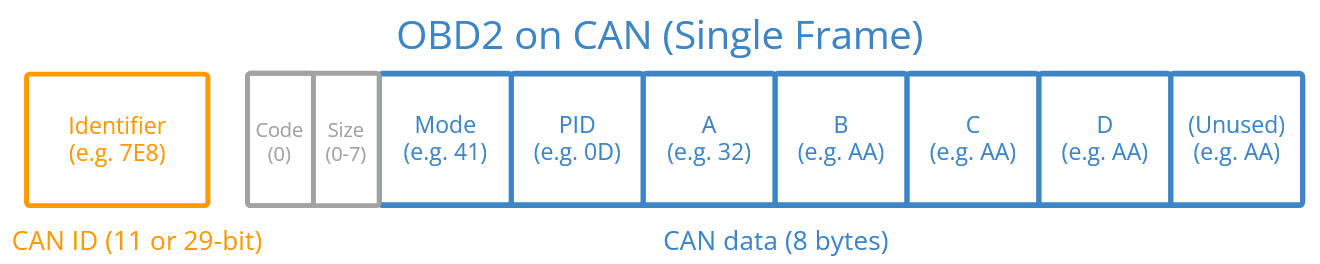
\includegraphics[width=0.8\textwidth]{OBD-frame.png}
  \caption{Format d'una trama \acro{obd-ii}}
  \label{fig:OBD-frame}
  \end{figure}

\begin{itemize}
  \item \textbf{Identificadors}: Com ja s'ha comentat a l'apartat dedicat a l'ISO-15765-4, els identificadors utilitzats per a la comunicació amb 
  l'equip de diagnosi estan predefinits i són fixes. S'utilitza l'identificador 0x7DF per enviar so\l.licituds genèriques a qualsevol 
  \acro{ecu}, mentre que les respostes arriben des d'\acro{ecu}s específiques utilitzant identificadors que van del 7E8 al 7EF corresponent la primera a l'\acro{ecu}
  principal responsable del motor.
  
  \item \textbf{Code i Size}: Aquests camps són heretats directament del protocol ISO-TP.
  
  \item \textbf{Mode}: Aquest byte especifica l'acció que es vol dur a terme amb el missatge \acro{pid}. Hi ha un total de 10 modes estàndard, que van des del 
  01 fins al 0A. En les respostes, el mode indicat és el mateix però sumant-li 0x40. Per exemple, una petició amb mode 01 tindrà una resposta amb mode 41.
  
  \item \textbf{PID}: Aquest byte indica la consulta concreta que es vol realitzar. Existeix una llista de \acro{pid}s estàndard definida per el SAE J1962
  (com ara \acro{pid} 0C per a les revolucions del motor). Tot i que són estàndard, no tots els vehicles han d'implementar tots els \acro{pid}s.
  
  \item \textbf{A, B, C, D (Dades)}: Els següents bytes contenen les dades de resposta. Cada \acro{pid} defineix com s'han d'interpretar aquests bytes. 
  Per exemple, per al \acro{pid} 0C (\acro{rpm}), els bytes A i B s'utilitzen per calcular les revolucions del motor amb la fórmula:

  \[
  \text{RPM} = \frac{(A \times 256) + B}{4}
  \]
\end{itemize} 

\subsection{Modes}

Com hem vist, els missatges \acro{obd-ii} inclouen un mode que defineix el tipus d'acció que es vol realitzar en la comunicació amb les \acro{ecu}s del vehicle. 
Cada mode té una funció específica, i en alguns casos, no cal especificar un \acro{pid}. A continuació es detallen els principals modes 
definits per l'estàndard:

\begin{itemize}
  \item \textbf{Mode 1}: Permet consultar dades en temps real del vehicle segons el \acro{pid} indicat, com ara la velocitat, la temperatura del refrigerant, 
  la posició del pedal d'accelerador, etc.
  
  \item \textbf{Mode 2}: Consulta les dades guardades en un \textit{Freeze Frame}, que són els valors de certs paràmetres en el moment exacte en què es va 
  registrar un \acro{dtc}. Només disponible si hi ha un error registrat.
  
  \item \textbf{Mode 3}: Envia una petició a totes les \acro{ecu}s per tal que retornin els \acro{dtc} actius que tenen emmagatzemats. Aquest mode no requereix 
  cap \acro{pid} i sol ser utilitzat per a diagnòstic general de fallades.
  
  \item \textbf{Mode 4}: Serveix per esborrar els \acro{dtc}s guardats i apagar la llum \acro{mil}. Si el problema persisteix, l'\acro{ecu} el tornarà a 
  registrar i la llum es tornarà a encendre. Tampoc cal especificar cap \acro{pid}.
  
  \item \textbf{Mode 5}: Permet consultar els resultats dels tests dels sensors d'oxigen (O2) en vehicles que no utilitzen la xarxa \acro{can}. El \acro{pid} 
  indica quin banc i sensor es vol consultar.

  \item \textbf{Mode 6}: Ofereix resultats dels tests monitoritzats realitzats per l'\acro{ecu}, coneguts com a \textit{On-Board Monitoring Tests}. El contingut 
  pot variar segons el fabricant i el vehicle, però s'utilitza per accedir a resultats de diagnosi avançada, com el funcionament del catalitzador 
  o del sistema \acro{egr}. El \acro{pid} identifica el test o component concret.
  
  \item \textbf{Mode 7}: Mostra \acro{dtc}s pendents o no confirmats, que són errors detectats però que encara no han superat els criteris per ser considerats 
  com a confirmats. No encenen la \acro{mil} però poden indicar problemes intermitents. No cal especificar \acro{pid}.
  
  \item \textbf{Mode 8}: Permet activar o desactivar actuadors del vehicle (com vàlvules, relés, ventiladors, etc.) per fer proves. El \acro{pid} indica 
  quin actuador es vol provar. No tots els vehicles implementen aquest mode.
  
  \item \textbf{Mode 9}: Ofereix informació del vehicle, com el \acro{vin} (\textit{Vehicle Identification Number}), l'identificador del calibratge de l'\acro{ecu} i altres dades 
  de fabricació. El \acro{pid} identifica el tipus d'informació desitjada.
  
  \item \textbf{Mode 10}: Retorna els \acro{dtc}s permanents, que són errors que no poden ser esborrats simplement amb el mode 4, i només desapareixen 
  quan el sistema ha validat que el problema ja no hi és durant diversos cicles de conducció. No cal \acro{pid}. 
\end{itemize} 

\subsection{Exemple pràctic d'ús d'un PID}

Per i\l.lustrar el funcionament pràctic dels missatges \acro{obd-ii}, es mostra a continuació un exemple de consulta a un \acro{pid} concret: la lectura de les \acro{rpm} del motor 
mitjançant el \acro{pid} 0C en Mode 1 (lectura de dades en temps real).

\textbf{Missatge de sol·licitud}

\begin{itemize}
  \item \textbf{ID}: 0x7DF.
  
  \item \textbf{Dades}: 02 01 0C 00 00 00 00 00.
\end{itemize} 

\textbf{Interpretació}

\begin{itemize}
  \item \textbf{02}: Nombre de bytes útils que segueixen (2 bytes)
  
  \item \textbf{01}: Mode 1, consulta de dades en temps real.
  
  \item \textbf{0C}: \acro{pid} de lectura de les revolucions del motor.
\end{itemize} 

\textbf{Missatge de resposta}

\begin{itemize}
  \item \textbf{ID}: 0x7E8 (\acro{ecu} del motor).
  
  \item \textbf{Dades}: 04 41 0C 0F A0 00 00 00.
\end{itemize} 

\textbf{Interpretació:}

\begin{itemize}
  \item \textbf{04}: Nombre de bytes útils de resposta.
  
  \item \textbf{41}: Resposta al mode 1 (01 + 0x40 = 0x41).
  
  \item \textbf{0C}: Confirma que la resposta correspon a la consulta realitzada.

  \item \textbf{0F A0}: Valors codificats que representen les revolucions del motor (en decimal 15 i 160).
\end{itemize} 

Per obtenir el valor de les \acro{rpm} a partir dels bytes A i B (0F i A0 en hexadecimal), s'utilitza la fórmula següent:

\[
\text{RPM} = \frac{(A \times 256) + B}{4} = 1000\ \text{RPM}
\]

\subsection{Altres protocols de comunicació utilitzats per l'OBD-II}

Tot i que actualment el protocol \acro{can} és l'estàndard de facto per a la comunicació \acro{obd-ii}, aquest no va ser l'únic protocol utilitzat. 
Abans de la seva obligació legal al 2008, molts fabricants  implementaven altres protocols compatibles amb el connector \acro{obd-ii}. Aquests protocols 
alternatius varien en la seva arquitectura i velocitat de transmissió, i encara es poden trobar en vehicles fabricats abans de la generalització del \acro{can}. 
A continuació es descriuen aquest protocols breument, amb les prpietats especificades a aquesta referencia \cite{sparkfun_obd2}:

\begin{itemize}
  \item \textbf{ISO 9141-2 (K-Line)}: Utilitzat principalment en vehicles europeus i asiàtics abans de la introducció del protocol \acro{can}. Funciona a 10,4 kb/s i utilitza 
  una línia de comunicació anomenada \textit{K-Line}, amb suport opcional per a una segona línia (\textit{L-Line}).
  
  \item \textbf{ISO 14230-4 (KWP2000)}: És una evolució de l'ISO 9141-2. Manté la velocitat de 10,4 kb/s. Pot operar amb una o dues línies, igual que el seu predecessor.
  
  \item \textbf{SAE J1850 VPW (Variable Pulse Width)}: Protocol adoptat per General Motors, utilitza una sola línia de comunicació i també transmet a 10,4 kb/s.

  \item \textbf{SAE J1850 PWM (Pulse Width Modulation)}: Utilitzat per Ford, és més complex perquè funciona amb dues línies i arriba a velocitats de fins a 41,6 kb/s, 
  oferint millor rendiment a costa d'un cablejat més complicat.
\end{itemize} 

\subsection{Detalls no estandards de l'OBD-II}

Tot el que s'ha explicat fins ara fa referència a l'estàndard que els fabricants de vehicles estan obligats a seguir. A partir d'aquest punt, però, 
els fabricants tenen llibertat per implementar modificacions que poden alterar el comportament esperat del sistema. En aquest apartat es presenten 
alguns dels aspectes més rellevants que escapen a l'estandardització. Com a inspiracio per aquest apartat s'ha consultat \cite{youtube_canreality} i \cite{can_vehicle_systems}

\subsubsection{Estructura del bus}

En una explicació simplificada, es podria pensar que totes les \acro{ecu}s d'un vehicle estan connectades a un únic bus 
\acro{can} i que, a través del port \acro{obd-ii}, és possible accedir lliurement a tots els missatges d'aquesta xarxa. En la pràctica, això rarament és així. 
Els fabricants solen restringir l'accés a la informació estrictament necessària per complir amb la normativa, i no mostren dades addicionals del vehicle.

Això implica que la xarxa \acro{can} a la qual accedim des del port \acro{obd-ii} no està connectada directament a totes les \acro{ecu}s. En lloc d'això, hi ha un 
dispositiu intermediari (\textit{gateway}), que filtra i controla els missatges disponibles des del port de diagnosi. En aquesta figura \ref{fig:car_structure} es pot veure 
un exemple simplificat de l'estructura real d'un sistema de comunicació dins d'un vehicle.

\begin{figure}
\centering
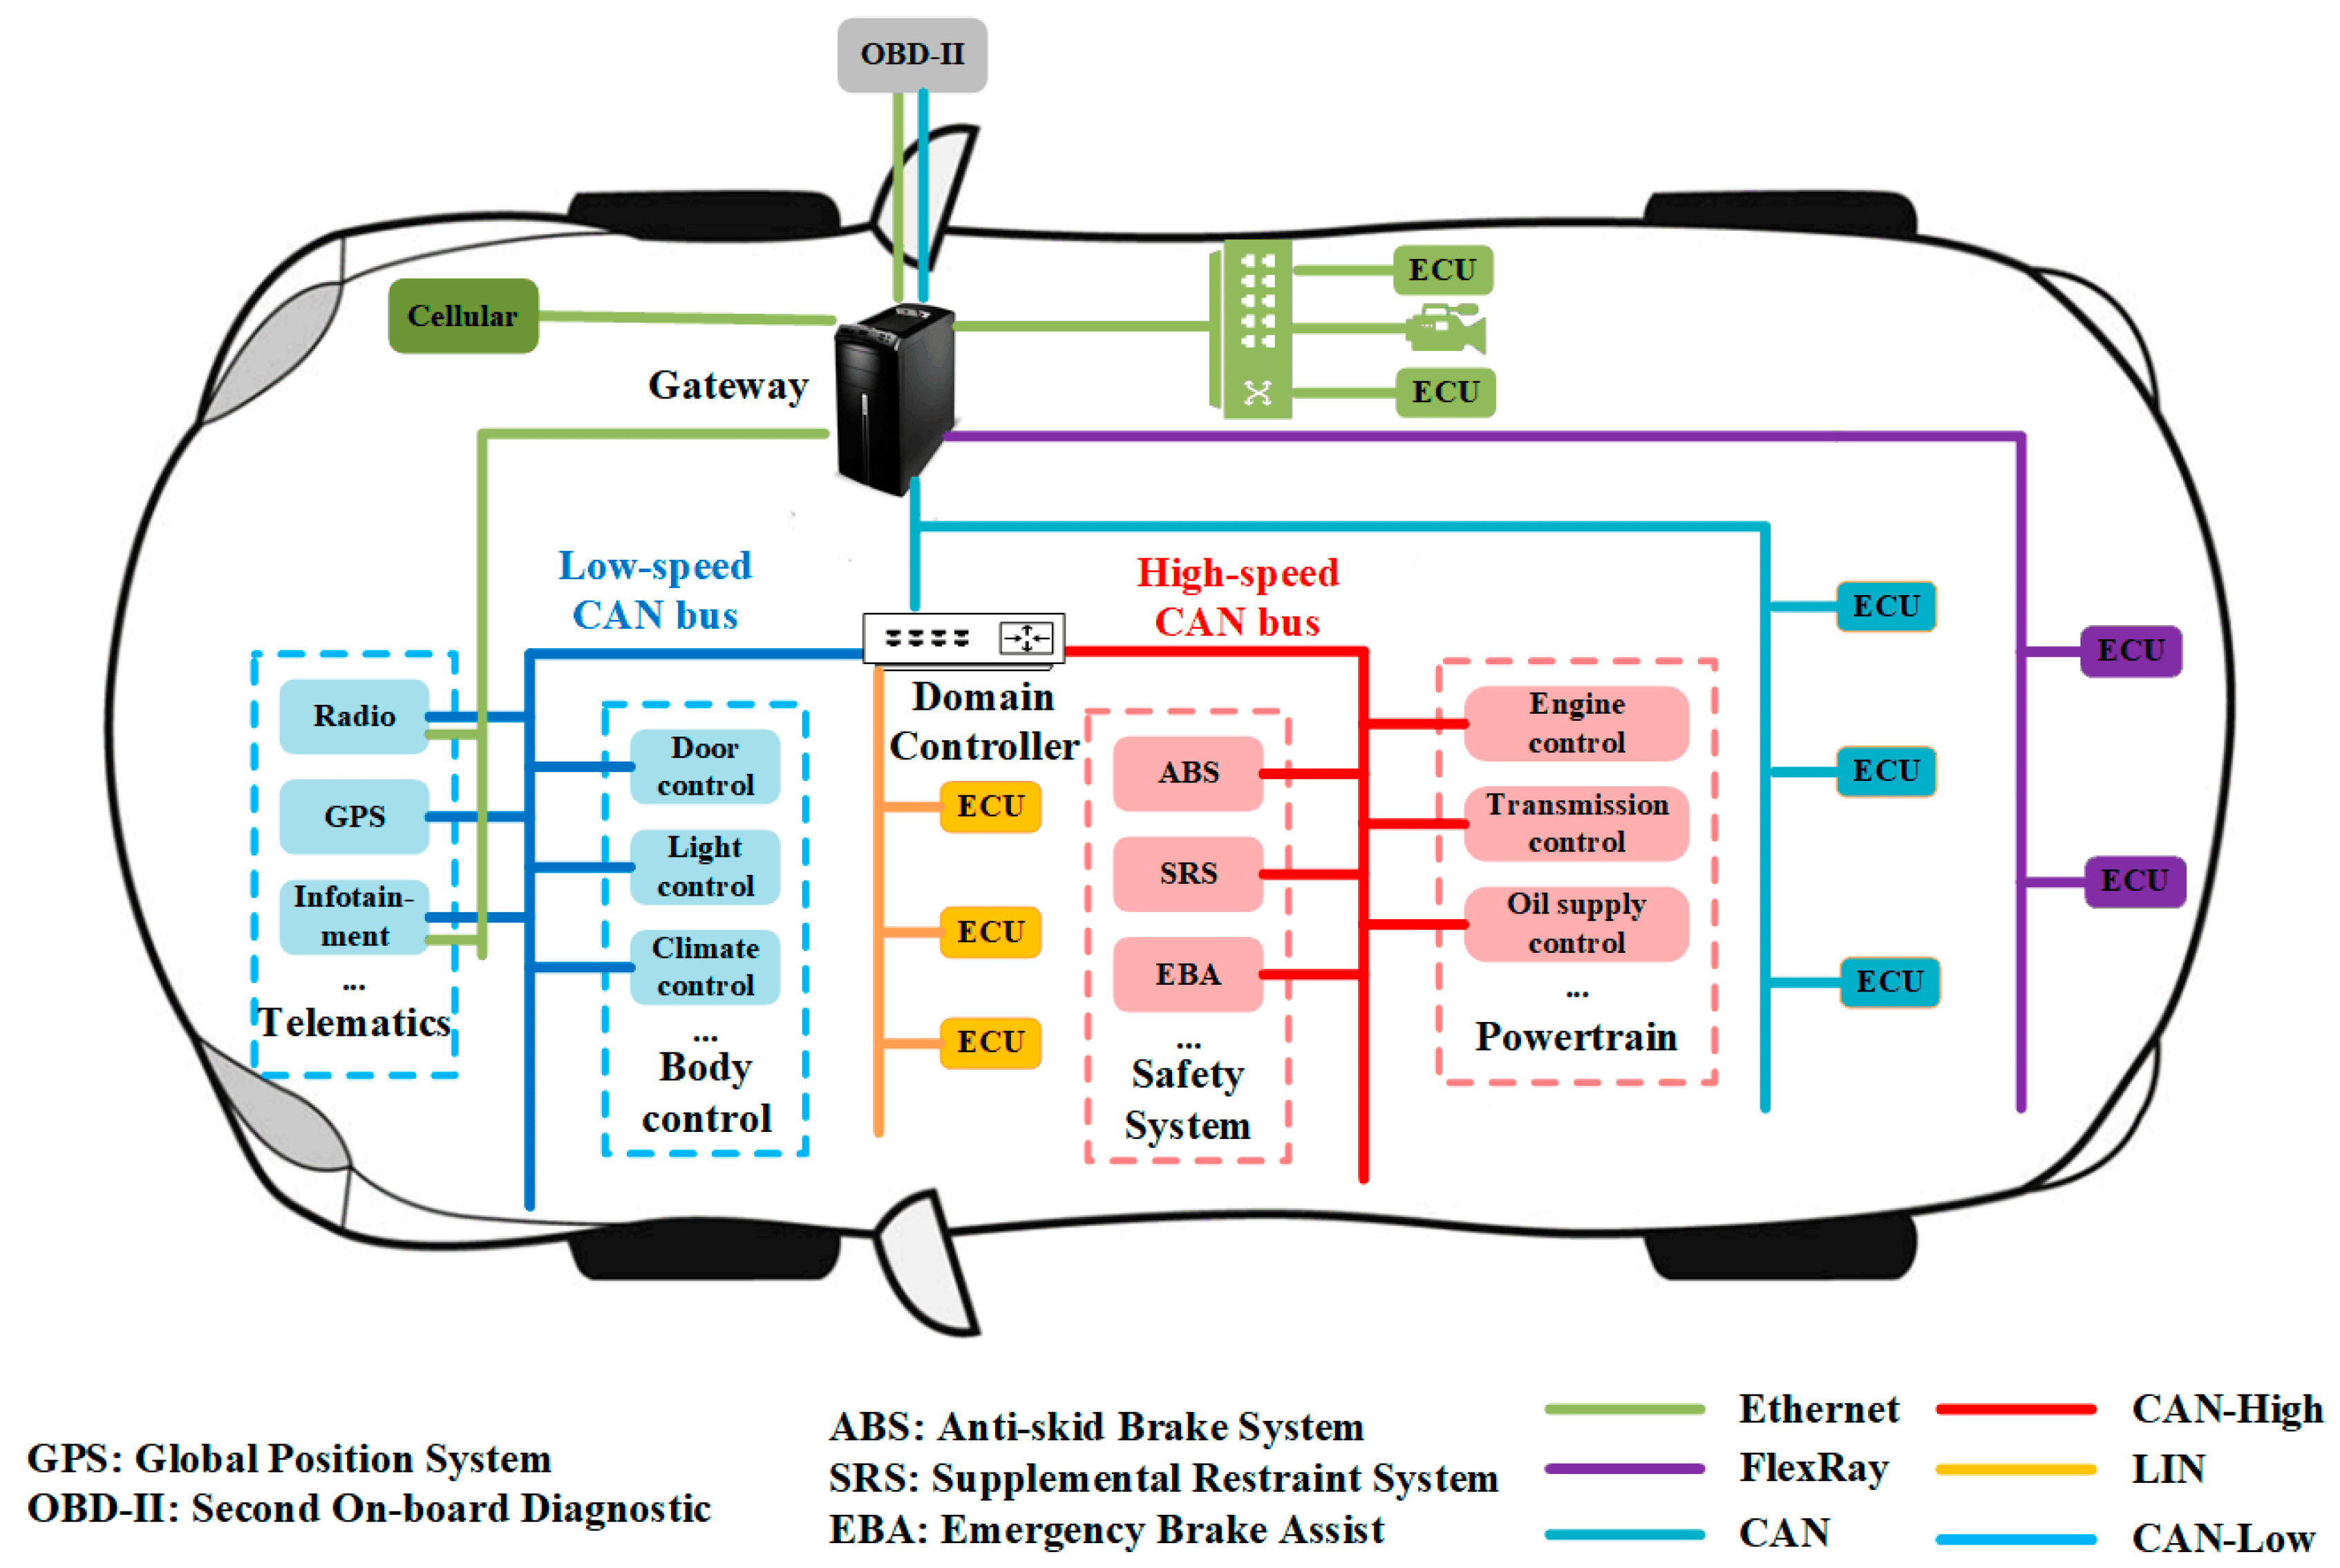
\includegraphics[width=0.8\textwidth]{car_structure.png}
\caption{Estructura real de les comunicacions d'un vehicle}
\label{fig:car_structure}
\end{figure}

Com s'observa a la figura, les diferents \acro{ecu}s poden estar connectades a xarxes separades que no necessàriament utilitzen el mateix protocol \acro{can} del \acro{obd-ii}. 
Els fabricants seleccionen el protocol més adequat segons els requisits de cada sistema, normalment entre els que es mencionen a \cite{softing_protocols}. 
Els protocols més destacats, a part del \acro{can} i les seves variants, són:

\begin{itemize}
  \item \textbf{LIN (Local Interconnect Network)}: Utilitzat per a sistemes de baixa velocitat i menor criticitat, com els controls de finestres, 
  seients o miralls.
  
  \item \textbf{FlexRay}: Present en vehicles d'alta gamma, permet comunicació d'alta velocitat i gran fiabilitat per a sistemes com la suspensió 
  activa o la direcció assistida electrònica.
  
  \item \textbf{Ethernet automotriu}: Cada cop més estès, gràcies a la seva alta velocitat de transmissió util per dispositius com càmeres.

  \item \textbf{MOST (Media Oriented Systems Transport)}: Dissenyat per a l'integració de sistemes multimèdia i d'entreteniment.
\end{itemize} 

Aquest conjunt de busos no forma una única xarxa contínua, sinó diverses xarxes separades interconnectades mitjançant \textit{gateways}. Aquests dispositius actuen 
com a ponts i filtres, poden: transmetre informació entre busos, traduir protocols i, sobretot, limitar l'accés a certs missatges per motius de seguretat, 
privacitat o protecció de la propietat inte\l.lectual.

Els fabricants tenen diversos motius per limitar la visibilitat de la informació interna del vehicle:

\begin{itemize}
  \item \textbf{Seguretat}: Per evitar l'accés no autoritzat a sistemes crítics com els frens o el motor.
  
  \item \textbf{Protecció de propietat intel·lectual}: Per impedir que tercers accedeixin a missatges que puguin revelar algoritmes propietaris de control.
  
  \item \textbf{Control comercial}: Per forçar l'ús d'eines oficials de diagnosi i serveis tècnics autoritzats per realitzar operacions avançades.
\end{itemize} 

Finalment, el port \acro{obd-ii}, tot i tenir 16 pins físics, només en fa servir uns quants per al protocol \acro{can} segons la normativa, tal i com s'ha vist, mentre que 
els pins restants poden ser utilitzats de manera propietària per accedir a altres busos o funcionalitats específiques. Això permet als fabricants connectar línies de comunicació internes, 
o donen acces a connexions reservades per a tasques de manteniment o programació. Com que aquests usos no estan estandarditzats, el contingut real del connector \acro{obd-ii} 
varia segons el fabricant, limitant l'accés de l'usuari a només la part visible i regulada per la normativa. Així, tot i la presència d'un connector estàndard, 
l'accés complet a la xarxa interna del vehicle, composta per diverses \acro{ecu}s distribuïdes en diferents busos, continua sent parcial i fortament controlat.

\subsubsection{Restriccions d'identificadors i mecanismes de protecció}

Tal com s'ha comentat anteriorment, els fabricants de vehicles apliquen diverses mesures per restringir l'accés a la comunicació amb les \acro{ecu}s a través del port \acro{obd-ii}. 
Tot i que moltes unitats de control podrien, en teoria, comunicar-se amb l'exterior, la informació disponible està fortament limitada i protegida.

Una de les tècniques més habituals és l'ús d'\acro{id}s i estructures de missatge no estandarditzades, que varien entre fabricants. Fora del mínim 
requerit per la normativa \acro{obd-ii}, la resta de la comunicació pot estar codificada, xifrada o basada en protocols interns no documentats. Això dificulta enormement 
la interpretació o la reproducció dels missatges sense disposar d'informació tècnica específica del fabricant.

Quan s'utilitzen eines de monitorització per escoltar el trànsit del bus \acro{obd-ii}, és habitual detectar gran quantitat de trames de les quals se'n desconeix el 
significat o la font. En alguns casos, aquests missatges poden estar protegits amb algoritmes d'autenticació o xifratge, impedint així la interacció directa 
fins i tot si es coneix l'\acro{id}.

Una tècnica bàsica d'enginyeria inversa per descobrir la funcionalitat d'algunes trames és el mètode \textit{record and replay}. Aquest consisteix a activar manualment una 
funció del vehicle (com moure un seient o encendre llums), observar els missatges generats i intentar reenviar-los per comprovar si es reprodueix la mateixa acció. 
No obstant això, aquest mètode sovint no és efectiu en sistemes moderns, ja que molts dispositius integren mecanismes de validació addicionals o estan protegits per 
\textit{gateways} que bloquegen trames no autoritzades.

Una de les tècniques de protecció més esteses és la autenticació per \textit{Seed-Key}, utilitzada per habilitar comandes sensibles. Aquest sistema funciona de la següent manera:

\begin{enumerate}
    \item El client envia una petició d'accés a l'\acro{ecu}.
    \item L'\acro{ecu} respon amb una clau variable anomenada \textit{seed}.
    \item El client ha de calcular la resposta correcta (\textit{key}) mitjançant un algorisme específic.
    \item Si la clau és vàlida, l'\acro{ecu} activa temporalment l'accés a funcionalitats avançades.
\end{enumerate}

S'ha consultat aquesta referencia \cite{openeecu_seedkey} per aquesta explicació,

\chapter{Comunicació externa}

Per la transmissió de missatges remots necessitem vàries eines que ens permetin, tenir accés a la xarxa a utilitzar i el protocol adient per realitzar les 
comunicacions per a la nostra aplicació.

\section{Connexió a la xarxa mòbil}

Una de les opcions més adients per garantir la connectivitat en mobilitat és l'ús de xarxes mòbils ce\l.lulars. Aquest tipus de xarxa permet mantenir una comunicació 
persistent mentre el vehicle es desplaça, i és ideal per a aplicacions que requereixen l'enviament de dades en temps real. A continuació es fa una breu 
explicció de com s'aconsegueix l'acces a la xarxa, per a major documentacio consultar \cite{wikipedia_gsm}, \cite{adslzone_apn} i \cite{datascientest_pdp}.

El funcionament bàsic d'aquesta infraestructura es basa en la connexió del dispositiu a una xarxa d'un operador mitjançant estacions base, o antenes de comunicació. 
Aquestes estacions configuren una xarxa de cobertura que opera amb diferents generacions de tecnologia mòbil (2G, 3G, 4G o 5G). La transmissió de dades s'efectua 
mitjançant ones de ràdio i tècniques de modulació.

Per establir aquesta comunicació, el dispositiu ha d'incloure un mòdul compatible amb la tecnologia utilitzada per l'operador. Aquest mòdul requereix una 
targeta \acro{sim} (\textit{Subscriber Identity Module}), que actua com a identificador exclusiu de l'usuari dins la xarxa mòbil. La \acro{sim} conté informació crítica com l'\acro{imsi} 
(\textit{International Mobile Subscriber Identity}), claus criptogràfiques per garantir la seguretat de la comunicació i la configuració de l'\acro{apn} (\textit{Access Point Name}), 
que determina el punt de connexió a Internet dins la xarxa de l'operador.

Una vegada autenticat el dispositiu a través de la \acro{sim} (\textit{Subscriber Identity Module}), s'estableix una connexió de dades mitjançant un context \acro{pdp} (\textit{Packet Data Protocol}), que actua com un 
túnel virtual cap a la xarxa de l'operador. En aquest procés, el dispositiu rep una adreça \acro{ip}, permetent així la comunicació amb servidors externs mitjançant 
protocols de xarxa com \acro{tcp/ip}. A partir d'aquí, és possible utilitzar protocols d'aplicació com \acro{mqtt} per enviar i rebre dades en temps real amb sistemes remots.

\subsection{Comunicació amb un modul sim}

Per gestionar les funcionalitats d'un mòdul \acro{sim} s'utilitza un conjunt d'instruccions conegudes com a comandes \acro{at} (\textit{Attention Commands}). Aquestes ordres es 
transmeten des d'un microcontrolador o dispositiu host cap al mòdul mitjançant una interfície sèrie. El mòdul interpreta la comanda, realitza l'operació 
corresponent i retorna una resposta. S'ha consultat la següent referenecia \cite{onomondo_at} per aquesta apartat.

Existeix un estàndard internacional, definit per la 3GPP, que estableix un conjunt de comandes \acro{at} bàsiques que tots els mòduls han de suportar. Aquestes comandes 
permeten realitzar operacions essencials com verificar la comunicació amb el mòdul, controlar les trucades, gestionar missatges \acro{sms}, etc. Un exemple senzill és la 
comanda \acro{at}. Quan s'envia aquesta comanda, el mòdul ha de respondre amb OK, la qual cosa indica que hi ha comunicació correcta entre el dispositiu host i el mòdul \acro{uart}.

Les comandes \acro{at} tenen una estructura estàndard que permet consultar, configurar o executar funcions específiques del mòdul. Els formats més habituals són els següents:

\begin{itemize}
  \item \textbf{AT+X}: Executa una acció o operació immediata relacionada amb la funció X. S'utilitza quan no cal passar cap paràmetre, només activar la funcionalitat.
  
  \item \textbf{AT+X=?}: Consulta quins valors admet com a paràmetres una comanda determinada. Aquesta forma ajuda a descobrir els valors vàlids abans de configurar.
  
  \item \textbf{AT+X?}: Consulta el valor actual configurat per la funció X. És útil per veure l'estat del sistema o la configuració sense modificar-la.
  
  \item \textbf{AT+X=<valor>}: Assigna un valor o paràmetre a una configuració determinada. És el format més comú per modificar el comportament del mòdul.
\end{itemize} 

A més de les comandes estàndard, molts fabricants implementen comandes \acro{at} específiques o propietàries que permeten accedir a funcionalitats avançades pròpies de cada 
model. Aquestes comandes poden incloure la gestió de connexions a Internet mitjançant protocols \acro{tcp/ip} o \acro{http}, la configuració de funcionalitats \acro{gnss} o \acro{gps} i altres.

Aquestes comandes no estan regulades per cap organisme internacional i poden variar significativament entre fabricants, fet que fa imprescindible consultar el manual 
de comandes \acro{at} específic del dispositiu emprat en cada cas.

És habitual que per a comandes més complexes s'utilitzin comandes \acro{at} dobles que requereixen un input posterior després de la comanda inicial. En aquests casos, la primera comanda 
indica que s'està a punt d'enviar dades i el mòdul respon amb un caràcter especial (com >) que indica que està preparat per rebre l'entrada de l'usuari. 

\section{MQTT}

Per tal que diferents dispositius puguin accedir a les dades enviades pel dispositiu del nostre vehicle, necessitem un protocol de comunicació lleuger, eficient i capaç de gestionar 
múltiples accessos. En aquest context, el protocol \acro{mqtt} (\textit{Message Queuing Telemetry Transport}) és una opció òptima per a la nostra aplicació, especialment en entorns amb recursos 
limitats i connexions de xarxa mòbil. Per a consultar la documentació complerta consultar \cite{oasis_mqtt}, a continuacio es fa una breu explicació amb informació extreta de \cite{wikipedia_mqtt}.

\acro{mqtt} és un protocol de la capa d'aplicació, dissenyat específicament per a la transmissió eficient de dades entre dispositius en xarxes amb amplada de banda limitada o latència variable. 
Es tracta d'un protocol orientat a la comunicació \textit{machine-to-machine} i \textit{Internet of Things} (IoT), caracteritzat per la seva lleugeresa, simplicitat i fiabilitat.

El seu funcionament es basa en un model de publicació/subscripció, que permet una comunicació flexible i desacoblada entre múltiples dispositius. El sistema es compon de dues entitats principals:

\begin{itemize}
  \item \textbf{Clients MQTT}: Dispositius que poden publicar dades o subscriure's a dades.
  
  \item \textbf{Broker MQTT}: Servidor central que rep tots els missatges publicats i els distribueix als clients que estiguin subscrits als \textit{topics} corresponents.
\end{itemize} 

Els \textit{topics} són etiquetes jeràrquiques utilitzades per organitzar la informació. Un client que vol rebre certa informació es subscreix a un tòpic determinat, mentre que un client que vol enviar 
dades publica un missatge en aquell tòpic. El broker actua com a intermediari i s'encarrega de distribuir els missatges de manera eficient a tots els clients subscrits.

Gràcies a aquestes característiques, \acro{mqtt} ens permet transmetre de manera remota i fiable les dades recollides pel sistema \acro{can} del vehicle. Podrem organizar la informació provinent del vehicle 
en \textit{topics}.

\chapter{Arquitectura del dispositiu}

Per al funcionament del nostre sistema es descriuen tots els components principals necessaris per al dispositiu que volem desenvolupar. La solució, esta basada en altres projectes similars com
els que es poden consultar a les següents referencies \cite{lastminute_can}, \cite{openvehicles} i \cite{youtube_hackcar}.

\begin{figure}
  \centering
  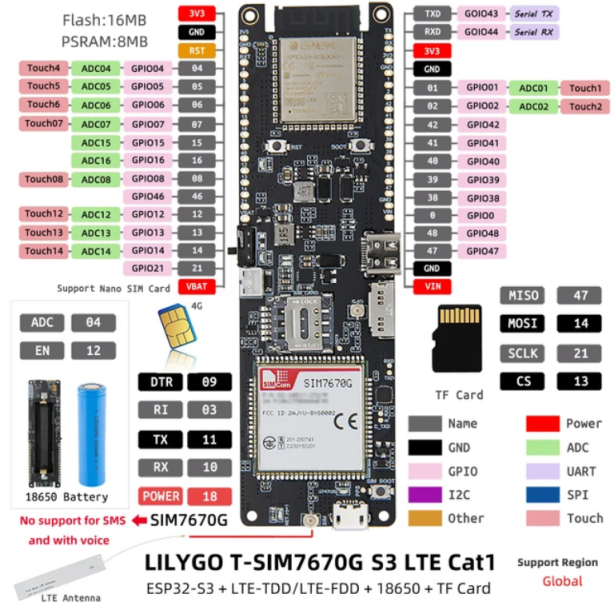
\includegraphics[width=0.8\textwidth]{ESP32.png}
  \caption{Pinout i caracteristiques de la placa de desenvolupament de la placa ESP32 utilitzada}
  \label{fig:ESP32}
  \end{figure}

\begin{itemize}
  \item \textbf{Microprocessador amb placa de desenvolupament}: Necessitem un microprocessador capaç de gestionar les comunicacions entre els diferents components. Aquest ha de poder processar 
  missatges del bus \acro{can} i mantenir una comunicació eficient via \acro{mqtt}. El processador escollit és l'ESP32, conegut pel seu baix consum energètic i la seva idoneïtat per a aplicacions \textit{IoT} a 
  petita escala, com la nostra. A més, en ser àmpliament utilitzat, disposa d'una gran comunitat i suport, amb moltes eines i llibreries disponibles que faciliten el desenvolupament.

  En concret, hem optat per la variant ESP32-S3-WROOM-1, que incorpora diverses millores resppecte una ESP convencional. Es pot consultar el seu datasheet compelrt a \cite{espressif_esp32s3}.
  Hem escollit aquesta variant perque vam trobar-la junt a una placa de desenvolupament que integra diversos components clau per al nostre sistema, cosa que redueix la necessitat de mòduls externs.
  En aquesta referencia es poden apreciar detalls sobre la placa \cite{lilygo_sim7670g}. A la figura \ref{fig:ESP32}, es mostra tot el que incorpora la placa de desenvolupament , sent els perifèrics destacats els següents:

  \begin{itemize}
    \item \textbf{Controlador CAN}: L'ESP32 no incorpora un controlador \acro{can} complet, ja que no pot gestionar els nivells de voltatge del bus. Tot i això, inclou un controlador \acro{twai} 
    (\textit{Two-Wire Automotive Interface}), que és la implementació del protocol \acro{can} per part d'ESP. Aquest s'encarrega de gestionar tota la lògica del protocol, però necessitem un component 
    extern per a la conversió de voltatges.
  
    \item \textbf{Mòdul SIM i suport per antena}: La nostra placa de desenvolupament incorpora un mòdul SIMCom 7670G, que ofereix connexió a xarxes mòbils 3G i 4G. Es pot consultar el datasheet a \cite{simcom_a7670}.
    Aquest mòdul implementa comandes \acro{at} per gestionar connexions \acro{mqtt}, tal com requereix el nostre disseny. La configuració dels pins és la següent: el pin \acro{gpio} 18 s'utilitza per activar el mòdul, mentre que la comunicació sèrie 
    s'estableix mitjançant els pins \acro{gpio} 11 (TX) i \acro{gpio} 10 (RX). Per garantir el funcionament òptim del mòdul, la placa inclou:

    Ranura per a targeta \acro{sim}, que permet la connexió a la xarxa mòbil.

    Connexió per a antena \acro{lte} externa, inclosa al kit essencial per a la comunicació. Es tracta d'una antena \textit{Full Band LTE} (698-960 MHz / 1710-2690 MHz), compatible amb la majoria de bandes 
    mòbils utilitzades pels operadors.

  \end{itemize} 
  \item \textbf{Connector OBD-II}: Aquest connector és el que ens permet accedir a les comunicacions del vehicle. Necessitem un connector que ens proporcioni els senyals necessaris: 
  tant el \acro{can} \textit{ High} com el \acro{can} \textit{Low} per a les comunicacions, així com el voltatge de la bateria i el \acro{GND} per alimentar el nostre dispositiu. En el nostre cas, hem optat per un cable 
  que dóna accés directe als 16 pins del connector \acro{obd-ii}.
  
  \item \textbf{Transceptor CAN}: Com s'ha mencionat, el controlador \acro{can} de l'ESP32 no suporta els voltatges del protocol \acro{can}. Per adaptar els nivells de senyal de 3.3V (amb els quals 
  treballa l'ESP32) als nivells del bus \acro{can} del vehicle, utilitzem un transceptor \acro{can}, concretament el SN65HVD230. Aquest dispositiu converteix els senyals digitals generats pel controlador 
  \acro{twai} en senyals diferencials compatibles amb el bus \acro{can} (normalment amb una referència de 2.5V, on \acro{can} \textit{High} i \acro{can} \textit{Low} osci\l.len per sobre i per sota d'aquest valor). Podeu consultar el 
  \textit{datasheet} aquí \cite{ti_sn65hvd230}
  
  \item \textbf{Convertidor DC-DC (Buck Converter)}:

  El port \acro{obd-ii} del vehicle proporciona una tensió de 12V, estàndard en la majoria de vehicles lleugers. No obstant això, la placa ESP32 funciona internament a 3.3V i pot ser alimentada 
  per l'entrada Vin, que accepta tensions al voltant de 5V.

  Per això, necessitem un mètode eficient per reduir la tensió de 12V a un valor adequat per a la nostra placa. Aquí entra en joc el convertidor DC-DC tipus \textit{buck}. Un \textit{buck converter} és 
  un regulador de commutació que redueix la tensió d'entrada de manera altament eficient. A diferència dels reguladors lineals, que dissipen l'energia 
  sobrant, el buck converter la converteix de forma més eficient. Com ha referenica s'ha utlitzat aquesta proposta \cite{espboards_power}.

  En el nostre projecte, hem optat per un mòdul basat en l'MP1584EN, un convertidor compacte que accepta tensions d'entrada entre 4.5V i 28V i proporciona una sortida ajustable entre 0.8V i 
  25V (amb un màxim de 3A). Es configura per a obtenir 5V a la sortida i alimentar el pin Vin de l'ESP32. consultar el datashhet coomplert consultar \cite{all_datasheet_mp1584en}.
\end{itemize} 

\section{Disseny de la placa}

Amb l'objectiu d'integrar totes les funcionalitats necessàries per al nostre sistema, s'ha considerat imprescindible el disseny d'una placa electrònica personalitzada. Actualment no existeix 
un dispositiu comercial que incorpori tots els components requerits pel projecte, motiu pel qual s'ha optat per desenvolupar una solució pròpia a partir de mòduls ja existents.

La placa dissenyada actua com una shield per a diversos elements, i ha estat concebuda per facilitar tant la fabricació com el muntatge. En aquest sentit, es tracta d'un disseny d'una sola capa, 
utilitzada també com a pla de massa, i amb components majoritàriament de muntatge \acro{thl} per simplificar el procés de soldadura. L'única excepció és el transceptor \acro{can}, que és de tipus \acro{smd}.

Els principals elements integrats a la placa són els següents:

\begin{itemize}
  \item \textbf{Suport per a l'ESP}: S'han disposat dues files de 16 pins per allotjar la placa de desenvolupament ESP32.
  
  \item \textbf{Muntatge del convertidor DC-DC}: Aquest mòdul s'integra directament a la placa mitjançant soldadura.
  
  \item \textbf{Integració del transceptor CAN}: El circuit inclou el transceptor soldat directament sobre la placa amb les connexions corresponents. A més, s'incorpora una resistència de 
  $10k\ \Omega$ per controlar millor els pendents de pujada i baixada del senyal al bus \acro{can}.
  
  \item \textbf{Connexió del cable OBD-II}: S'ha previst un connector tipus screw terminal per facilitar la connexió de 4 dels 16 fils procedents del cable \acro{obd-ii}. D'aquesta manera, es poden 
  establir les connexions amb el bus \acro{can} (\acro{can} High i \acro{can} Low) i l'alimentació de la batería del vehicle.
\end{itemize} 

Pel que fa a les connexions internes:

\begin{itemize}
  \item El screw terminal permet l'entrada dels senyals \acro{can} \textit{High} i \acro{can} \textit{Low}, així com l'alimentació procedent del connector \acro{obd-ii}.
  
  \item El convertidor DC-DC transforma la tensió de la bateria del vehicle i proporciona alimentació a l'ESP a través del pin Vin.
  
  \item L'ESP32 alimenta el transceptor CAN amb 3,3 V, i estableix la comunicació a través dels pins \acro{gpio} 15 i 16, utilitzats com a RX i TX respectivament.
\end{itemize} 

Per realitzar el disseny hem utilitzat l'eina KiCad. Per a una documentació completa, podeu consultar la pàgina oficial \cite{kicad}. 

Aquesta eina ens permet dissenyar l'esquema elèctric de la nostra placa a partir dels elements disponibles al programari. Un cop planificat l'esquema elèctric, hem d'assignar a cada element un 
footprint, és a dir, el component físic exacte que utilitzarem a la nostra placa. En el nostre cas utilitzem element THL per a una major facilitat en la soldadura.

Amb tots els components assignats, passem al disseny de la \acro{pcb}. En aquesta fase determinem el tamany de la placa, el nombre de capes, planifiquem les connexions entre components mitjançant pistes 
i via, i distribuïm els elements.

Un cop finalitzat el disseny, podem generar els fitxers Gerber, que són els arxius estàndard utilitzats pels fabricants per produir la placa. Aquests fitxers contenen informació detallada 
sobre les pistes, les perforacions entre d'altres. En aquesta figura \ref{fig:PCB} mostren tant l'esquema elèctric com el disseny final de la \acro{pcb}.

  \begin{figure}
  \centering
  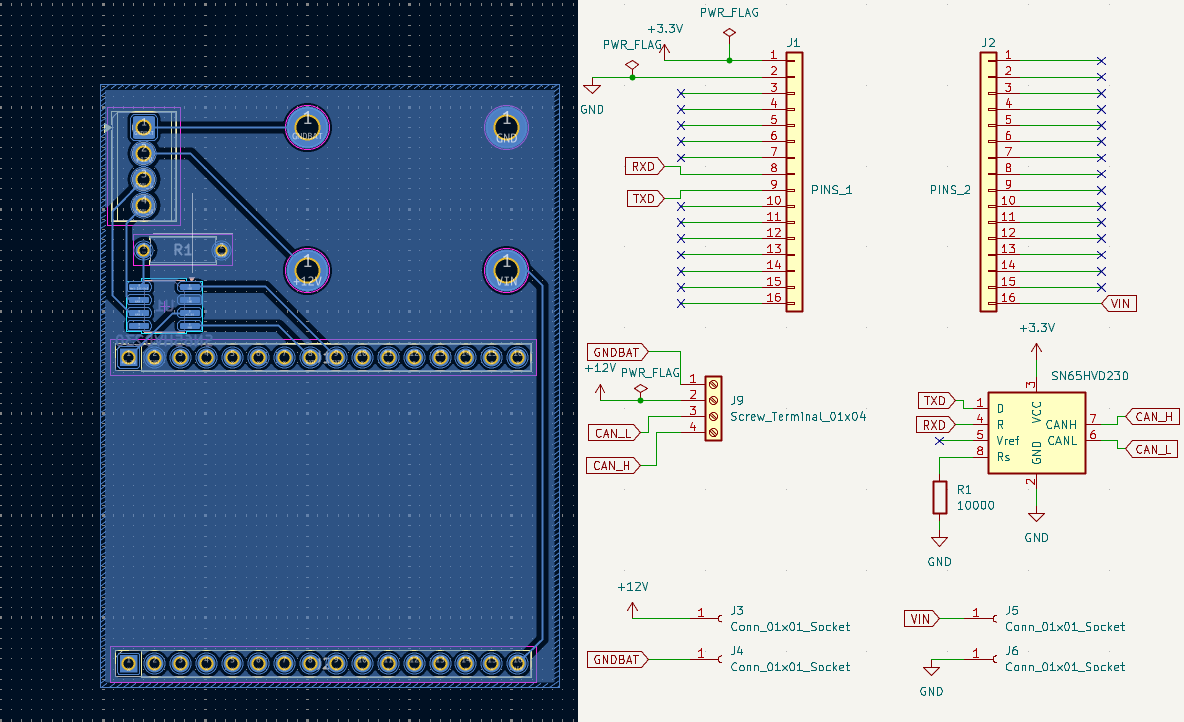
\includegraphics[width=0.8\textwidth]{PCB.png}
  \caption{PCB i esquema electrònic de la placa dissenyada}
  \label{fig:PCB}
  \end{figure}

\chapter{Implementació de software}

A continuació es redacta tota la documentació necessària per entendre la implementació de programari realitzada pel funcionament del sistema.

\section{Entorn de programació}

Per al desenvolupament del projecte s'ha escollit l'entorn ESP-IDF (\textit{Espressif IoT Development Framework}), que proporciona un conjunt complet de llibreries i eines específiques per a 
dispositius basats en microcontroladors ESP, com el que s'utilitza. Aquest \textit{framework} està implementat en llenguatge C, fet que permet una programació de baix nivell, amb un control 
directe sobre el maquinari, es pot consultar la documentació a \cite{espressif_docs}.

Un aspecte fonamental d'ESP-IDF és el suport natiu per al sistema operatiu FreeRTOS, que facilita la gestió de múltiples processos o tasques en para\l.lel. Aquesta característica és essencial en el 
projecte, ja que cal executar diferents processos de manera concurrent, per separar i gestionar les comunicacions de forma independent. La documentació de la llibreria esta disponible a \cite{freertos}

Per a la gestió del projecte utilitzem l'eina PlatformIO, que s'integra perfectament amb ESP-IDF. PlatformIO ofereix una sèrie de funcionalitats avançades com ara la gestió automàtica de dependències, 
la configuració modular del projecte, així com eines per a la compilació, depuració i monitoratge del sistema. La pagina de suport es pot cosultar a \cite{platformio}

\section{Comunicació SIM}

Per a la gestió de la comunicació de comandes \acro{at} amb el nostre mòdul \acro{uart}, cal una correcte gestió de una comunicació \acro{uart} amb aquest. S'ha d'alimentar el modul mitjançant 
el pin \acro{gpio} 18 i comunicar-nos utilitzant TX al gpio 11 i rx al 10, com s'ha comentat anteriorment. Per a aquesta tasca s'utilitza la llibreria de l'entorn ESP-IDF \cite{espressif_uart}

\subsection{Comandes AT necessaries}

Per a la comunicació \acro{mqtt} mitjançant un mòdul \acro{uart} de la mateixa família que el nostre, s'ofereix documentació per a realitzar la següent seqüència al document següent \cite{simcom_mqtt}.

Algunes comandes difereixen lleugerament a causa de la nostra variant de mòdul \acro{uart}; en concret, aquí \cite{simcom_at} hi ha la documentació completa de les comandes \acro{at} suportades pel nostre 
dispositiu.

A continuació, expliquem breument totes les comandes utilitzades, així com els seus paràmetres i la resposta esperada en cas que es retorni alguna cosa més a part d'OK:

\subsubsection{Comprovació del mòdul SIM} 
Aquest conjunt de comandes serveix per assegurar-se que el mòdul està actiu, que la \acro{uart} està inserida i desbloquejada, i que es disposa de senyal de 
xarxa suficient per a la comunicació.
\begin{itemize}
  \item \textbf{AT}: Comanda bàsica per comprovar si el mòdul respon correctament.

  \item \textbf{AT+CPIN=/AT+CPIN?}: S'insereix el valor del PIN en la primera comanda com a paràmetre, i en la segona es corrobora que la \acro{uart} ha quedat desbloquejada.

  \item \textbf{AT+CSQ}: Retorna la qualitat del senyal de ràdio. Concretament, retorna un valor de 0 a 31 de RSSI, que indica la potència del senyal rebut (un valor acceptable seria al 
  voltant de 10--20, que equival a -93~dBm a -73~dBm), i un valor de Bit Error Rate, normalment 0.

  \item \textbf{AT+CREG?}: Comprova si el dispositiu està registrat a la xarxa GSM. Es retorna si rebem notificacions de la xarxa (en el nostre cas, valor 0) i l'estat; un valor de 1 indica 
  que estem correctament registrats.

  \item \textbf{AT+CGREG?}: Comprova l'estat de registre a la xarxa GPRS. Es retorna si rebem notificacions de la xarxa (valor 0) i l'estat; un valor de 1 indica que estem correctament registrats.
  
  \item \textbf{AT+CPSI?}: Retorna informació detallada del sistema de xarxa: mode del sistema, mode d'operació, codi de país mòbil (MCC), codi de xarxa mòbil (MNC), codi d'àrea de localització 
  (LAC), identificador de ce\l.la (\text{Cell \acro{id}}), número absolut de canal de ràdio (RF ChNum), nivell de senyal rebut (RxLev), ajust de l'osci\l.lador local (Track LO Adjust), i paràmetres C1-C2.
\end{itemize}

\subsubsection{Comandes per al context PDP} 
Aquestes comandes configuren i activen el context \acro{pdp}.
\begin{itemize}
  \item \textbf{AT+CGDCONT=}: Defineix un context \acro{pdp}, establint el tipus de connexió de dades i l'APN del proveïdor. Defineix l'identificador del context, el tipus \acro{pdp} (habitualment \acro{ip}) 
  i l'APN, que és el nom d'accés proporcionat per l'operador mòbil.

  \item \textbf{AT+CGACT=/AT+CGACT?}: Activa o desactiva un context \acro{pdp} prèviament definit amb AT+CGDCONT. En aquest cas, s'activa amb el paràmetre 1, i es consulta posteriorment 
  si ha quedat activat.
\end{itemize}

\subsubsection{Configuració de la connexió MQTT} 
Aquest conjunt de comandes permet establir una connexió MQT.
\begin{itemize}
  \item \textbf{AT+CMQTTSTART}: Inicia el servei intern \acro{mqtt} del mòdul.ç
  
  \item \textbf{AT+CMQTTACCQ}: Crea una instància de client \acro{mqtt} amb un identificador i un nom assignat.
  
  \item \textbf{AT+CMQTTCONNECT}: Estableix connexió amb el broker \acro{mqtt}. Es necessita l'\acro{id} del client, la \acro{ip} o domini del broker, el port, el temps de \textit{keep-alive} i si volem mantenir la darrera sessió.
  
  \item \textbf{AT+CMQTTSUB}: Subscriu el client a un \textit{topic} per rebre missatges del broker. Inclou l'\acro{id}, el \textit{topic} i la qualitat del servei.
  
  \item \textbf{AT+CMQTTTOPIC}: Estableix el \textit{topic} on s'enviarà el missatge. Es passa l'\acro{id} i la longitud del \textit{topic}; el mòdul espera la inserció del \textit{topic} i retorna OK si és correcte.
  
  \item \textbf{AT+CMQTTPAYLOAD}: Defineix el missatge a publicar. Es passa l'\acro{id} i la longitud del missatge; el mòdul espera la inserció del missatge i retorna OK si és correcte.
  
  \item \textbf{AT+CMQTTPUB}: Publica el missatge prèviament definit. Els paràmetres són: \acro{id}, qualitat del servei i si volem retenir el missatge. Retorna l'\acro{id} i un codi d'error 0 si té èxit.
  
  \item \textbf{AT+CMQTTDISC}: Tanca la connexió amb el broker \acro{mqtt}. Es passa l'\acro{id} del client i el \textit{timeout}.
  
  \item \textbf{AT+CMQTTREL}: Elimina el client \acro{mqtt} creat prèviament. Es passa l'\acro{id} corresponent.
  
  \item \textbf{AT+CMQTTSTOP}: Finalitza el servei \acro{mqtt} al mòdul i allibera recursos.
\end{itemize}

\subsubsection{Altres respostes esperades} 
A partir de les connexions establertes, podem rebre missatges espontanis:
\begin{itemize}
  \item \textbf{+CMQTTCONNLOST}: Indica desconnexió passiva de la connexió \acro{mqtt}.
  
  \item \textbf{+CMQTTRXPAYLOAD}: Indica recepció d'un missatge en un \textit{topic} al qual el client està subscrit. Inclou informació addicional i el contingut del missatge.
\end{itemize}

\subsection{Mòdul AT\_Gestor}

Aquest fitxer s'encarrega de gestionar la comunicació per \acro{uart} amb el mòdul \acro{uart}, així com la transmissió i recepció de comandes \acro{at}. A continuació es 
descriuen les funcions implementades:

\begin{itemize}
  \item \texttt{void init\_sim(void)}: Encén el mòdul \acro{uart} i configura la comunicació \acro{uart}.

  \item \texttt{void write\_AT(const char *command)}: Escriu el contingut del buffer a través del bus \acro{uart}.

  \item \texttt{void read\_AT(char* rx\_buffer)}: Comprova si hi ha recepció per \acro{uart}; en cas afirmatiu, sobreescriu el buffer proporcionat 
  amb el missatge rebut.
\end{itemize}

A més, aquest fitxer incorpora directament totes les comandes \acro{at} necessàries per al funcionament del sistema, utilitzant la funció write\_AT. 
Aquestes comandes es finalitzen amb el caràcter de retorn de línia i nova línia (\textbackslash r\textbackslash n). Per exemple:

\begin{verbatim}
void AT(void) {
  write_AT("AT\r\n");
}
\end{verbatim}

\subsection{Mòdul MQTT\_Gestor}

Aquest fitxer treballa per sobre del mòdul \acro{at}. Aquí és on s'implementa la seqüència de comandes \acro{at} per establir la connexió \acro{mqtt}. Com que aquesta 
seqüència no és completament lineal, s'ha implementat com una màquina d'estats. En determinats casos, cal repetir part de la seqüència, per això, 
tot i no ser una màquina d'estats estricta (ja que no hi ha esdeveniments externs sinó respostes a comandes), s'ha optat per aquest enfocament per 
simplicitat i falta de coneixement d'altres solucions més sofisticades.

A continuació es descriu la seqüència de connexió, que també es pot consultar a la figura \ref{fig:state_machine} generada amb Mermaid \cite{mermaid}.

\begin{figure}
  \centering
  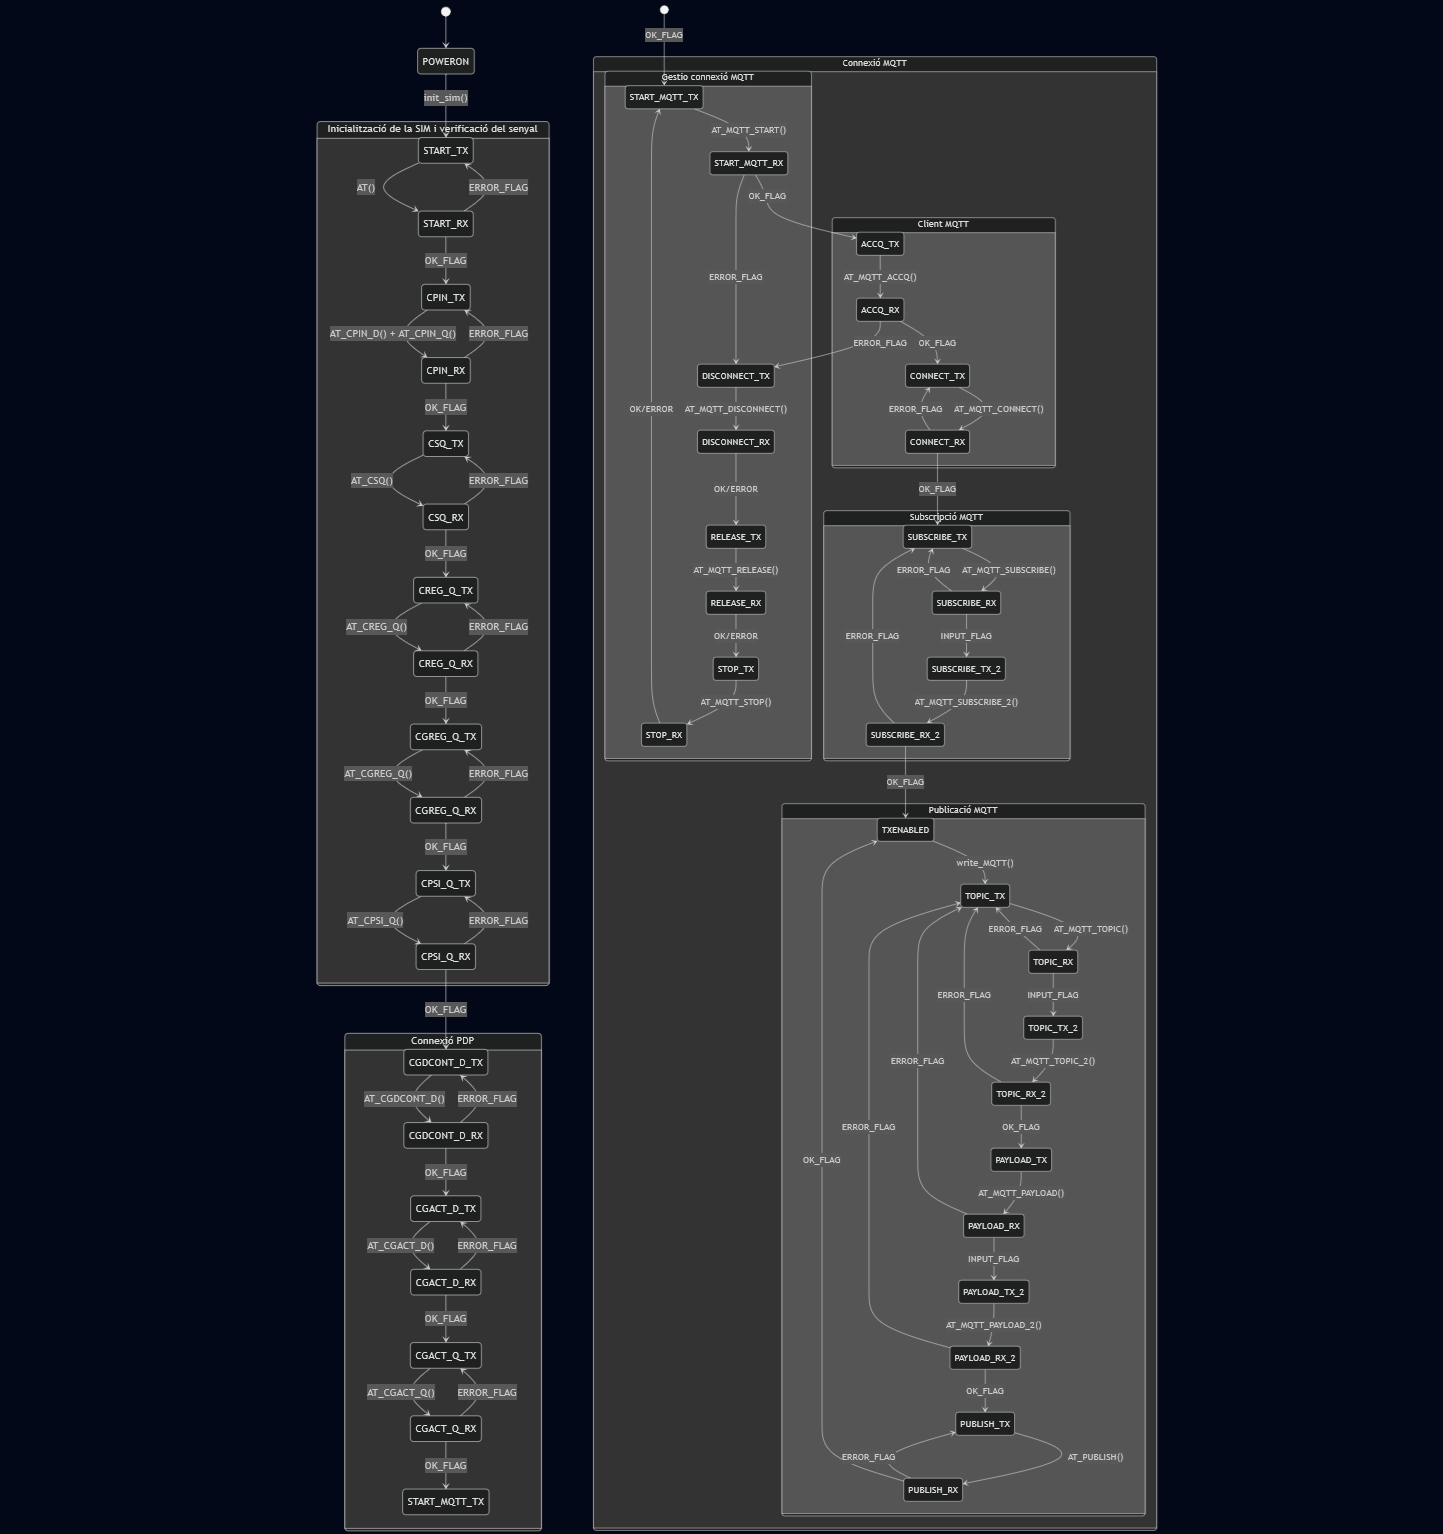
\includegraphics[width=0.8\textwidth]{state_machine.png}
  \caption{Màquina d'estats}
  \label{fig:state_machine}
  \end{figure}

La gestió de la seqüència segueix una estructura comuna: cada comanda consta de dos estats, un per l'enviament i un per la recepció de la resposta. 
Si la resposta és OK, es continua amb la següent comanda; si es detecta un error, es torna a enviar la mateixa comanda. En el cas d'instruccions 
que requereixen entrada de dades (com AT+CMQTTTOPIC o AT+CMQTTPAYLOAD), la seqüència s'amplia a quatre estats per gestionar l'entrada i 
la resposta adequadament. Si es produeix un error en qualsevol d'aquests passos, es retorna a l'inici de la seqüència corresponent.

\subsubsection{Excepcions a la lògica general}
\begin{itemize}
  \item \textbf{Inicialització del mòdul}: Simplement és un estat d'activació sense verificacions de resposta.

  \item \textbf{Gestió del PIN}: Per evitar errors quan la \acro{uart} ja està desbloquejada, s'envien consecutivament les comandes d'inserció (AT+CPIN) 
  i de consulta (AT+CPIN?), i només es valida la resposta d'aquesta darrera.

  \item \textbf{Error en AT+CMQTTSTART o AT+CMQTTACCQ}: Si aquestes comandes fallen, pot ser degut a un estat incoherent del client \acro{mqtt} 
  (Si no es va tancar correctament en una sessió anterior). En aquest cas, s'inicia una seqüència de neteja amb les comandes AT+CMQTTDISC, 
  AT+CMQTTREL i AT+CMQTTSTOP, independentment de si retornen error o no. Un cop completada, es torna a intentar la comanda 
  AT+CMQTTSTART.
\end{itemize}

Un cop establerta la connexió amb èxit, el sistema entra en l'estat TXENABLED, des del qual pot gestionar tres tipus d'esdeveniments:

\begin{itemize}
  \item \textbf{Recepció de missatge (+CMQTTRXPAYLOAD):} Quan es detecta aquest missatge, es desa el contingut rebut a una variable global per al seu 
  processament posterior.

  \item \textbf{Petició d'enviament MQTT:} Una funció externa, cambia l'estat correpsonent per iniciar la seqüència d'enviament d'un missatge \acro{mqtt}.

  \item \textbf{Pèrdua de connexió MQTT (+CMQTTCONNLOST):} Es detecta mitjançant la resposta rebuda i s'inicia una nova seqüència de connexió des de 
  la comanda AT+CMQTTSTART.
\end{itemize}

Un cop tractada la seqüència a implementar en aquest mòdul, es descriuen les funcions implementades:

\begin{itemize}
  \item void read\_AT\_processor(void): Prepara un buffer per comprovar si hi ha recepció des del mòdul \acro{uart} mitjançant la funció de recepció 
  del mòdul AT\_Gestor. Si és el cas, actualitza unes variables globals d'estat que indiquen si la resposta conté: OK, ERROR, 
  CMQTTCONNLOST o una petició d'entrada de dades (>). També comprova si s'ha rebut un +CMQTTRXPAYLOAD i, si és així, desa el 
  missatge a una variable global buffer\_mqtt.

  \item \texttt{void sim\_state\_machine(void)}: Implementa la seqüència de comandes \acro{at} mitjançant una màquina d'estats. Utilitza read\_AT\_processor 
  per gestionar les respostes i les funcions del mòdul AT\_Gestor per enviar les comandes.

  \item \texttt{bool read\_MQTT\_available(void)}: Comprova si buffer\_mqtt conté un missatge.

  \item \texttt{void read\_MQTT(char *message)}: Copia el contingut de buffer\_mqtt al buffer passat com a paràmetre i després el buida.

  \item \texttt{void write\_MQTT(const char* topic, const char* message)}: És una funció bloquejant que espera fins que la màquina d'estats estigui en 
  l'estat TXENABLED. Un cop s'hi troba, canvia l'estat a TOPIC\_TX, fet que inicia la seqüència d'enviament del missatge. Els paràmetres 
  s'emmagatzemen en variables globals que s'utilitzaran durant l'enviament.
\end{itemize}

\section{Comunicació CAN}

L'entron ESP-IDF té una llibreria preparada per gestionar el modul \acro{twai} que hem de gestionar per a la comunicació \acro{can}. La llibreria en concret es la que es troba en aquesta referencia 
\cite{espressif_twai}. Tot i aixi a continuació es fa un resum de les funcionalitats i pareametres principals:

\subsection{Configuració i ús del controlador TWAI}

La inicialització del controlador \acro{can} a ESP32 es realitza amb la funció:

\begin{verbatim}
esp_err_t twai_driver_install(const twai_general_config_t *g_config, 
                             const twai_timing_config_t *t_config, 
                             const twai_filter_config_t *f_config);
\end{verbatim}

Aquesta assigna els recursos del sistema i permet configurar tres blocs principals:

\subsubsection{Configuració general (twai\_general\_config\_t)}

Els paràmetres destacats són:

\begin{itemize}
    \item \texttt{controller\_id}: Identificador del controlador, útil amb per a mutiples instàncies de controlador en aquest dispositiu.
    \item \texttt{mode}: Mode de funcionament (normal, sense necessitat de \acro{ack} o només s'escolta sense actuar al bus).
    \item \texttt{tx\_io i rx\_io}: Pins \acro{gpio} utilizats per la transmissió i recepció.
    \item \texttt{tx\_queue\_len i rx\_queue\_len}: Mida de les cues de missatges.
    \item \texttt{sleep\_allow\_pd}: Permet que el controlador entri en mode de baix consum quan no està actiu, optimitzant l'ús d'energia.
\end{itemize}

En aquest projecte s'utilitza aquesta macro predefinida que configura valors bàsics per funcionament normal amb cues de 5 missatges:
\begin{verbatim}
TWAI_GENERAL_CONFIG_DEFAULT(tx_io, rx_io, mode)
\end{verbatim}

\subsubsection{Configuració de temporització (twai\_timing\_config\_t)}

Permet ajustar el \textit{bit timing} i la sincronització. Paràmetres clau:

\begin{itemize}
    \item \texttt{brp}: Divisor de freqüència que determina la durada d'un \emph{Time Quanta}. 
    \item \texttt{tseg\_1 i tseg\_2}: Definició de la durada en \acro{tq} d'aquest segments.
    \item \texttt{sjw}: Màxim nombre de \acro{tq} que es poden afegir o restar per corregir la sincronització
    \item \texttt{triple\_sampling}: Si està activat, el controlador farà tres mostrejos consecutius per a cada bit.
\end{itemize}

S'utilitza la configuració estàndard per treballar a 500 kbps:
\begin{verbatim}
TWAI_TIMING_CONFIG_500KBITS()
\end{verbatim}

\subsubsection{Configuració de filtre (twai\_filter\_config\_t)}

Permet limitar els missatges acceptats amb:

\begin{itemize}
    \item \texttt{acceptance\_code} i \texttt{acceptance\_mask}: Aquests dos paràmetres defineixen quins identificadors seran acceptats mitjançant una mascara.
    \item \texttt{single\_filter}: Indica si s'utilitza un únic filtre d'acceptació o si es poden configurar múltiples filtres.
\end{itemize}

S'utiliza aquesta macro per acceptar tots els missatges:
\begin{verbatim}
TWAI_FILTER_CONFIG_ACCEPT_ALL()
\end{verbatim}

\subsection{Transmissió de missatges}

La transmissió es realitza amb:

\begin{verbatim}
esp_err_t twai_transmit(const twai_message_t *message, TickType_t ticks_to_wait);
\end{verbatim}

Aquest afegeix el missatge a la cua de transmissió i espera que el bus estigui lliure. El paràmetre ticks\_to\_wait indica el temps 
màxim d'espera en cas que el bus estigui ocupat.

El format del missatge (twai\_message\_t) conté principalment:

\begin{itemize}
    \item \texttt{identifier}: \acro{id} del missatge (11 o 29 bits segons).
    \item \texttt{extd}: Indicador d'\acro{id} estàndard o estès.
    \item \texttt{rtr}: Indicador de trama de petició remota.
    \item \texttt{data\_length\_code} i \texttt{data[]}: Longitud i contingut de les dades.
\end{itemize}

\subsection{Recepció de missatges}

La recepció es gestiona amb:
\begin{verbatim}
esp_err_t twai_receive(twai_message_t *message, TickType_t ticks_to_wait);
\end{verbatim}

Es llegeix un missatge de la cua de recepció. Si no arriba cap missatge dins el temps definit, retorna ESP\_ERR\_TIMEOUT.

\subsection{Estat del sistema}

Una funció auxiliar rellevant per obtenir informació del controlador és:
\begin{verbatim}
esp_err_t twai_get_status_info(twai_status_info_t *status_info);
\end{verbatim}

Els camps més importants de twai\_status\_info\_t són:

\begin{itemize}
    \item \texttt{state}: Estat del controlador (parat, actiu, bus-off, recuperant).
    \item \texttt{msgs\_to\_tx} / \texttt{msgs\_to\_rx}: Missatges pendents de transmissió i recepció.
    \item \texttt{tx\_error\_counter} i \texttt{rx\_error\_counter}: Comptadors d'errors (\acro{tec} i \acro{tec}).
    \item \texttt{rx\_missed\_count} i \texttt{rx\_overrun\_count}: Missatges perduts en recepció per cua plena i sobrepassatje.
    \item \texttt{arb\_lost\_count}: Comptador de quantitat de comps que s'ha perdut l'arbitratge.
    \item \texttt{bus\_error\_count}: Comptador d'errors detectats al bus.
\end{itemize}

Aquests paràmetres són essencials per monitorar el correcte funcionament i evitar pèrdua de missatges.

\subsection{Mòdul CAN\_Gestor}

Aquest fitxer s'encarrega de gestionar les comunicacions \acro{can}. La seva implementació és mínima, ja que la major part de la funcionalitat prové 
directament de la llibreria utilitzada. A continuació es descriuen les funcions implementades:

\begin{itemize}
  \item \texttt{void init\_\acro{can}(void)}: Realitza la configuració necessària del perifèric \acro{twai} i l'inicialitza.

  \item \texttt{void write\_\acro{can}(int ID, int mode, int rtr, int payload\_length, uint8\_t* payload)}: Forma un missatge \acro{can} amb els paràmetres indicats i 
  l'envia a través del bus.

  \item \texttt{bool read\_\acro{can}(twai\_message\_t *message)}: Consulta si hi ha cap missatge disponible a la cua de recepció. Si és el cas, copia el missatge 
  rebut al buffer passat com a paràmetre.
\end{itemize}

A més, s'afegeixen dues funcions addicionals que fan ús de write\_\acro{can} per enviar missatges \acro{pid} específics per a la consulta de la velocitat del 
vehicle i de les revolucions per minut.

\subsection{Projecte sniffing i modul Sniffer\_Gestor}

Amb l'objectiu de dur a terme proves sistemàtiques sobre el bus \acro{can} del vehicle, es va integrar el projecte de codi obert canDrive disponible a \cite{github_candrive}. 
Aquesta eina, desenvolupada en Python, disposa d'una interfície gràfica (\acro{gui}) que permet monitorar 
en temps real els missatges \acro{can} rebuts a través d'una connexió \acro{uart}. En aquesta figura \ref{fig:Sniffing_GUI} s'aprecia una imatge de l'interfície.

\begin{figure}
  \centering
  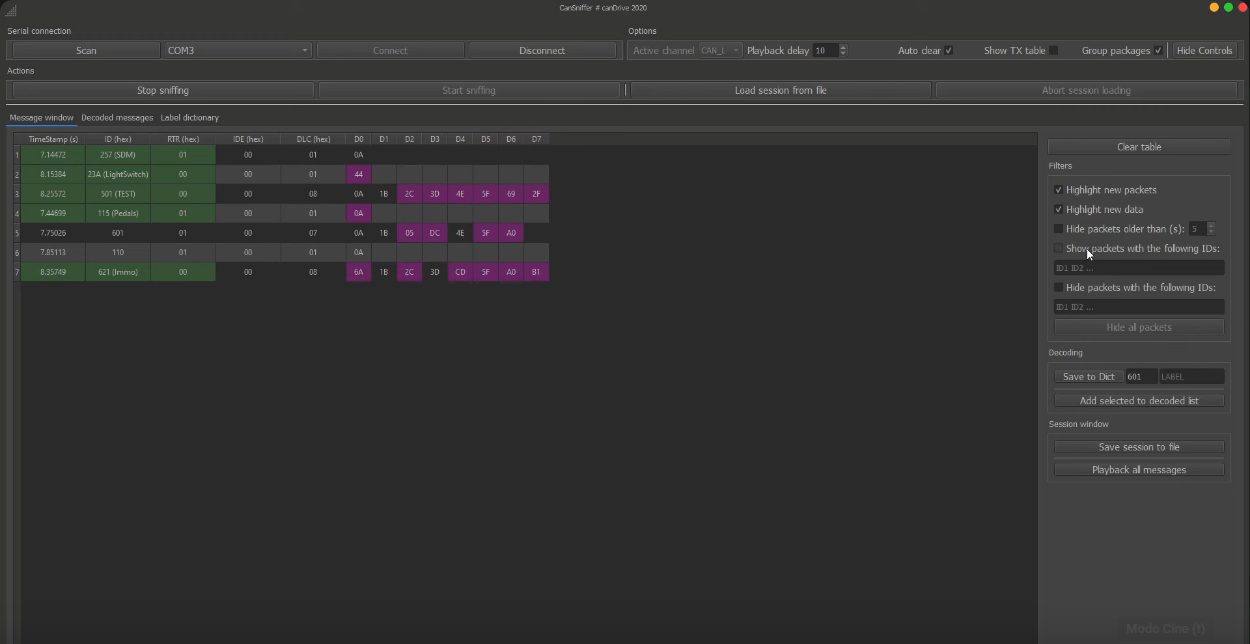
\includegraphics[width=0.8\textwidth]{Sniffing_GUI.png}
  \caption{GUI del projecte canDrive}
  \label{fig:Sniffing_GUI}
  \end{figure}

La \acro{gui} mostra els missatges agrupats per \acro{id} i actualitza automàticament el contingut quan s'arriben nous valors per un mateix identificador. Aquesta 
funcionalitat és especialment útil per a tasques d'enginyeria inversa, ja que permet identificar missatges generats per accions específiques del vehicle 
(com obrir finestres o activar intermitents) i verificar si aquests poden ser reproduïts.

Per tal de garantir la compatibilitat amb aquest programari, es va implementar el mòdul Sniffer\_Gestor, que adapta la sortida del dispositiu 
al format esperat pel projecte. El format utilitzat (consultable al fitxer canSniffer.ino del projecte) imprimeix cada missatge amb els camps \acro{id}, 
\acro{rtr}, \acro{ide} i DATA, separats per comes i finalitzats amb un salt de línia.

La funció principal del mòdul és:

\begin{itemize}
  \item \texttt{void print\_sniffing(twai\_message\_t message)}: Imprimeix per \acro{uart} la informació del missatge rebut segons l'estructura requerida pel 
  programari canDrive.
\end{itemize}

\section{Procés principal}

El procés principal s'encarrega de definir i gestionar els diferents processos relacionats amb les comunicacions \acro{can} i \acro{mqtt}, i d'enllaçar aquestes 
dues funcionalitats. A continuació es descriuen les funcions implementades:

\begin{itemize}
  \item \texttt{void write\_\acro{can}\_speeds(void)}: Aquesta funció s'encarrega d'enviar els missatges \acro{pid} de consulta de velocitat i revolucions, 
  espaiats per un interval de 5 segons.

  \item \texttt{void read\_\acro{can}\_processor(void)}: Crida la funció de recepció \acro{can}. Si hi ha un missatge disponible, es comprova si es tracta d'una 
  resposta a una consulta de velocitat o de revolucions. En cas afirmatiu, s'obté el valor corresponent i s'envia al servidor \acro{mqtt}.

  \item \texttt{void read\_MQTT\_processor(void)}: Crida la funció que verifica si el buffer de missatges \acro{mqtt} conté informació pendent. Si és 
  així, el missatge es mostra per pantalla. En aquest projecte no s'ha implementat cap funcionalitat addicional per a la recepció \acro{mqtt}, de manera 
  que no es realitza cap altra acció.
\end{itemize}

A partir d'aquestes funcions, es defineixen un total de tres processos:

\begin{itemize}
  \item \textbf{CAN\_task}: Inicialitza el mòdul \acro{can} i executa en bucle la funció read\_CAN\_processor.

  \item \textbf{MQTT\_task}: Executa en bucle la màquina d'estats del mòdul MQTT\_Gestor i, en cada iteració, crida la funció 
  read\_MQTT\_processor per comprovar si hi ha recepcions pendents.

  \item \textbf{Procés principal}: S'encarrega de definir i llançar els dos processos anteriors, i executa de manera cíclica la funció 
  write\_CAN\_speeds.
\end{itemize}

També s'ha implementat un mode de funcionament alternatiu, preparat per al projecte de \textit{sniffing}. Aquest mode s'activa mitjançant una 
macro i té com a objectiu desactivar l'enviament de \acro{pid}s i la comunicació \acro{mqtt}. En aquest cas, els missatges \acro{can} rebuts es mostren per pantalla, 
i el dispositiu actua únicament com un logger passiu de dades del bus \acro{can}.

\section{Client MQTT i Web}

Per tal de mostrar les dades de forma visual, es va desenvolupar un petit servidor web que actua com a subscriptor dels topics \acro{mqtt} del vehicle. 
Aquest servidor allotja una pàgina amb una interfície molt senzilla que mostra les dades en temps real.

\subsection{Broker MQTT}

Com a broker \acro{mqtt} es va utilitzar un dispositiu Ubuntu amb l’aplicació Mosquitto \cite{mosquitto}, que permet implementar un broker \acro{mqtt}. Es va utilitzar la configuracio
per defecte per al projecte.

Per tal de donar suport a l'accés públic del broker mitjançant una \acro{ip} externa, es va configurar el router de la xarxa per redirigir les peticions entrants al port 1883 (port per defecte 
del protocol \acro{mqtt}) cap a la \acro{ip} privada del dispositiu host, és a dir, la màquina Ubuntu amb Mosquitto. Aquest procediment es coneix com obrir un port.

\subsection{Servidor web}

El servidor web va ser desenvolupat utilitzant l'eina Flask, que és una llibreria de Python per al desenvolupament d'aplicacions web \cite{flask_docs}. 
Flask també disposa d'una extensió pròpia per gestionar comunicacions \acro{mqtt}, eina que també hem utilitzat \cite{flask_mqtt_docs}.

El codi de la part del servidor és força senzill. Es crea una aplicació bàsica amb Flask, es configuren els paràmetres necessaris per a la connexió \acro{mqtt} 
i es defineix la mateixa aplicació com a client \acro{mqtt}. L'aplicació està preparada per gestionar quatre possibles esdeveniments:

\begin{itemize}
  \item \textbf{Connexió MQTT}: Quan s'estableix la connexió amb el broker \acro{mqtt}, l'aplicació es subscriu als topics desitjats.
  
  \item \textbf{Recepció de dades MQTT}: En rebre un missatge d'un client \acro{mqtt}, es comprova el tema al qual pertany i es guarda el valor rebut en una 
  variable global que representa aquella magnitud (com la velocitat o les revolucions).
  
  \item \textbf{Accés web}: Quan un client web fa una petició d'accés a la branca principal (/), es carrega el fitxer \acro{html} corresponent.
  
  \item \textbf{Sol·licitud de dades}: Quan un client web fa una petició GET a la ruta /data, es retornen els valors de les variables globals 
  en format \acro{json}.
\end{itemize}

El servidor està allotjat en un ordinador portàtil dins de la xarxa domèstica, utilitzant una \acro{ip} pública i el port 5000. Per tant, no proporciona 
accés mitjançant un domini genèric. Tal com s'ha explicat a l'apartat anterior, s'ha redirigit el port 5000 del router cap a la \acro{ip} del dispositiu que 
allotja el servidor, per tal de permetre l'accés extern.

\subsection{Fitxers estàtics}

El document \acro{html} mostrat al navegador conté dos camps per visualitzar les dades. Per a l'estil visual s'utilitza el \textit{framework} Bootstrap. Per permetre 
l'actualització dinàmica de les dades, aquests camps estan marcats amb identificadors únics. En aquesta figura \ref{fig:Client_GIU} es pot apreciar el disseny de la
interfície

\begin{figure}
  \centering
  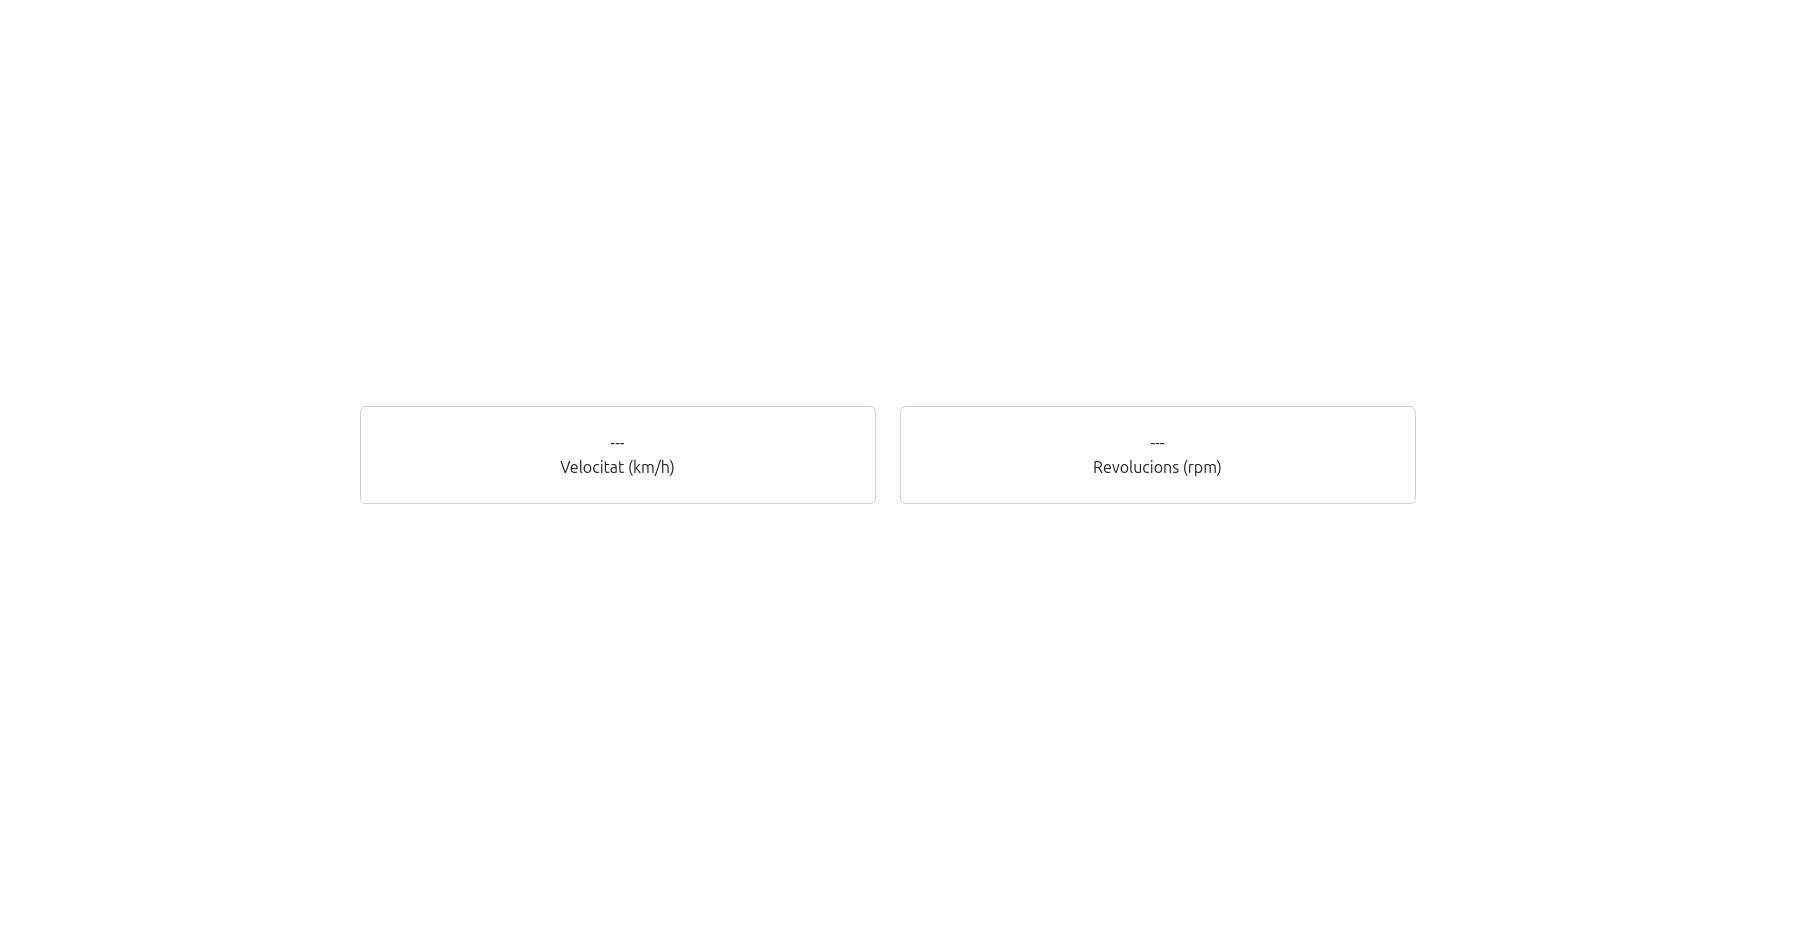
\includegraphics[width=0.8\textwidth]{Client_GIU.png}
  \caption{Interficie del client web}
  \label{fig:Client_GIU}
  \end{figure}

El fitxer JavaScript, que s'executa conjuntament amb l'\acro{html}, conté una funció que s'executa de manera periòdica cada 2 segons. Aquesta funció fa una 
petició a la ruta /data del servidor, espera la resposta i actualitza els camps d'informació de la pàgina web amb les dades rebudes.


\section{Estructura final del projecte}

El projecte complet es troba disponible al següent repositori de GitHub \cite{github_tfg}.

En aquest repositori es poden trobar els següents components:

\begin{itemize}
  \item \textbf{docs}: Conté els arxius necessaris per generar aquesta documentació utilitzant \LaTeX.

  \item \textbf{shield}: Inclou, per una banda, el projecte de KiCad de la \acro{pcb} i, per l'altra, els fitxers Gerber generats 
  a partir d'aquest projecte.

  \item \textbf{firmware}: Conté tot el codi i la documentació mencionats en aquest apartat, organitzats en els següents directoris:

  \begin{itemize}
    \item \textbf{ESP32-Remote-CAN}: Conté el projecte PlatformIO amb tot el codi destinat a l'ESP32.

    \item \textbf{MQTT}: Inclou diversos fitxers útils per a la consulta del broker \acro{mqtt}, fitxers de configuració per a Mosquitto, i els arxius 
    necessaris per a l'execució del servidor web.

    \item \textbf{Sniffing}: Conté el projecte \textit{sniffing}, amb tots els fitxers i documents necessaris per al seu funcionament.
  \end{itemize}
\end{itemize}

\chapter{Testeig}

A continuació es documenten totes les proves realitzades per aconseguir el funcionament complet del sistema.

\section{Comunicació SIM i MQTT}

Per verificar el funcionament del mòdul \acro{uart}, es va utilitzar una targeta \acro{uart} de la companyia Jazztel. Un cop identificats correctament els pins de comunicació del mòdul, es va emprar 
la seqüència de comandes \acro{at} requerida per establir una connexió exitosa amb el broker Mosquitto allotjat en una \acro{ip} pública.

Durant les proves, es va observar un comportament rellevant: el dispositiu, al no tancar explícitament la connexió \acro{mqtt}, mantenia la sessió oberta fins i tot després de desconnectar-se. Això 
provocava que, en intentar reconnectar-se, el sistema retornés un error degut a la sessió residual. Per solucionar-ho, es va incorporar a la seqüència una desconnexió forçada en cas de fallida 
en la connexió.

En un escari on només es vulguin enviar dades puntuals al servidor, seria possible tancar la connexió després de cada enviament. No obstant això, en aquest projecte també es volia mantenir la possibilitat 
de rebre missatges \acro{mqtt} en qualsevol moment, raó per la qual es va optar per deixar la connexió oberta i gestionar-ne els errors de reconnexió.

Un cop validada la comunicació \acro{mqtt}, es va comprovar el correcte funcionament del servidor web i el client desenvolupats. Es va confirmar que les peticions HTTP es 
gestionaven sense errors i que les dades proporcionades desde el mòdul \acro{uart} es mostraven en temps real a la interfície web.

\section{Comunicació CAN}

Per tal de verificar la comunicació amb el bus \acro{can} del vehicle, inicialment no es va fer ús del muntatge definitiu amb tots els components, sinó que es va optar per un sistema de 
proves improvisat que només incorporava els elements mínims necessaris. Aquest muntatge consistia en una ESP32 connectada a un mòdul transceptor \acro{can} (SN65HVD230 VP230) com el que es 
pot apreciar a aquesta figura \ref{fig:SN65HVD230-VP230}. La connexió física es realitzava mitjançant els terminals \acro{can} High i \acro{can} Low de la placa transceptora, connectats a través d'un screw terminal als 
cables del connector \acro{obd-ii}.

\begin{figure}
  \centering
  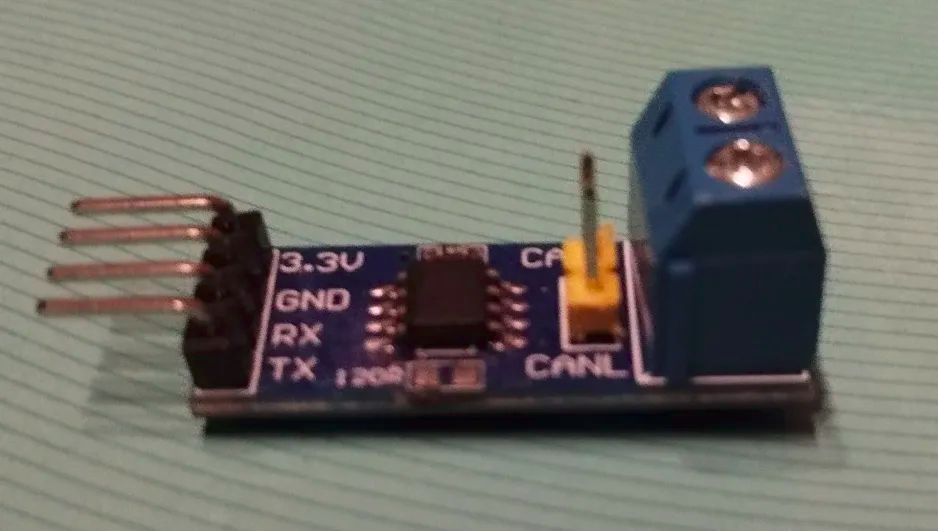
\includegraphics[width=0.8\textwidth]{SN65HVD230-VP230.png}
  \caption{Transmisor \acro{can} providional utilitzat}
  \label{fig:SN65HVD230-VP230}
  \end{figure}

Un aspecte important va ser la retirada de la resistència de $120~\Omega$ que la placa transceptora incorpora per defecte. Aquesta resistència només és necessària als extrems del bus \acro{can}, 
i com que el nostre dispositiu es connectava com a node intermedi, no havia de portar aquesta terminació.

Un altre detall rellevant fou localitzar físicament el port \acro{obd-ii} del vehicle. Aquest sol trobar-se a la zona inferior del quadre de comandament, habitualment sota el volant i sovint 
amagat rere una tapa de plàstic. Atès que la ubicació pot variar segons el fabricant i el model, cal consultar fonts específiques en línia per identificar-ne la posició exacta. En el 
cas del vehicle utilitzat el trobem a un compartiment rere una tapa d eplastic sota le volant com es veu a aquesta figura \ref{fig:localitzacio-obd}.

\begin{figure}
  \centering
  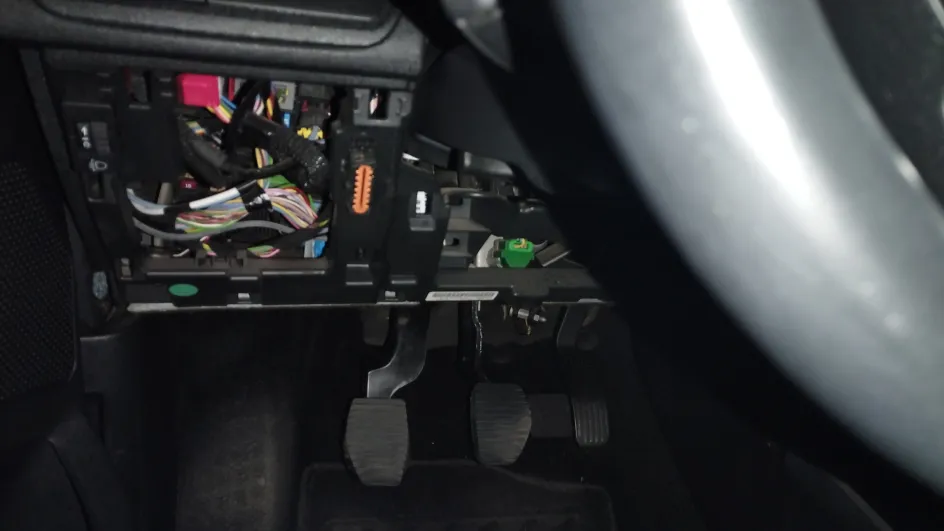
\includegraphics[width=0.8\textwidth]{localitzacio-obd.png}
  \caption{Localització del port \acro{obd-ii}}
  \label{fig:localitzacio-obd}
  \end{figure}

Per a facilitar les proves tmabé es va adquirir un connecor \acro{obd-ii} genèric, aquest dispositius estan dissenyats per accedir a la informació estàndard que proporciona el port \acro{obd-ii} dels vehicles. 
Aquests lectors, compatibles amb la majoria de protocols suportats per la normativa \acro{obd-ii}, permeten llegir i esborrar codis d'error \acro{dtc}, monitorar paràmetres en temps real 
i comprovar si el vehicle compleix amb els requisits d'emissions. La seva utilitat per l'entorn de proves és clau, ja que permeten verificar si el vehicle utilitza el protocol \acro{can}, 
identificar problemes de comunicació i assegurar que el sistema respon correctament abans d'interaccionar-hi amb dispositius propis.

Inicialment es va intentar fer les proves amb un Mitsubishi Space Star de l'any 2004. No obstant això, com que el protocol \acro{can} no va ser obligatori per als vehicles fins a l'any 2008, 
aquest model no el implementava, cosa que es va corroborar mitjançant un dispositiu de diagnosi genèric que indicava que el vehicle utilitzava un altre protocol, en concret la ISO 9141-2.

Per aquest motiu, es va buscar un vehicle alternatiu que garantís compatibilitat amb \acro{can}. El model escollit fou un Peugeot 2008 de primera generació (produït a partir de 2013), 
el qual sí que fa ús de \acro{can} com a protocol \acro{obd-ii} principal. La connexió es va fer amb èxit, però en una primera prova es van activar diverses alarmes al tauler del vehicle i es 
va encendre el testimoni MIL. Això indicava que el nostre dispositiu estava interferint amb el bus \acro{can}.

Mitjançant el lector \acro{obd-ii} generic es va poder llegir i esborrar el \acro{dtc} generat. El codi d'error indicava una interrupció total de la comunicació al bus, fet que suggeria un curt 
circuit o interferència greu. Es va descobrir que en retirar la resistència de terminació no s'havia fet correctament, provocant un curt entre \acro{can} High i \acro{can} Low. Aquesta situació es 
va verificar amb un tester al laboratori.

\begin{figure}
  \centering
  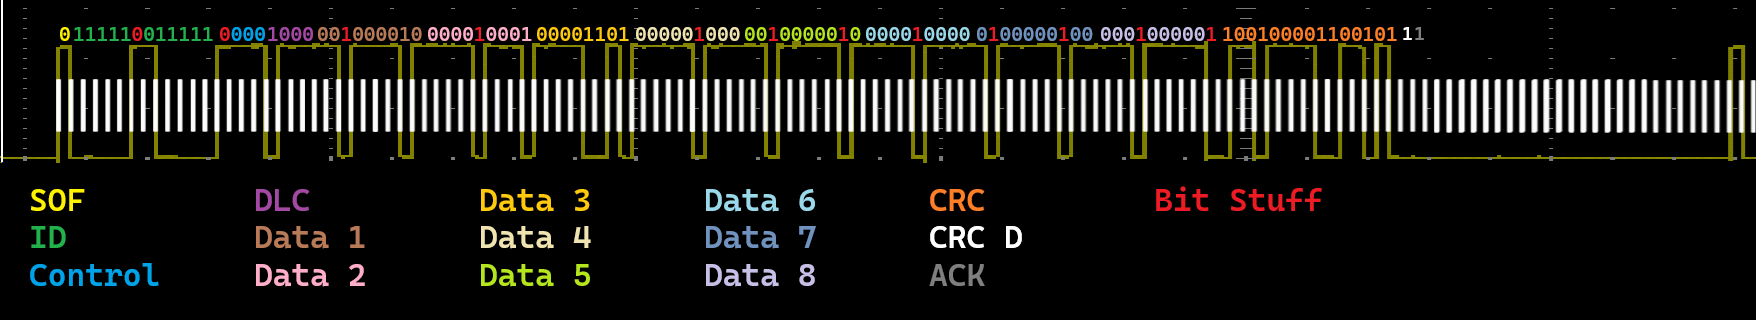
\includegraphics[width=0.8\textwidth]{CAN_Osciloscop.png}
  \caption{Captura d'una trama \acro{can}}
  \label{fig:CAN_Osciloscop}
  \end{figure}

Aprofitant la situació, es va procedir al laboratori a verificar mitjançant un osci\l.loscopi el correcte funcionament de tots els components implicats en la comunicació. 
Gràcies a això, es va obtenir una captura, que podem veure a la figura \ref{fig:CAN_Osciloscop}, on s'observa una trama \acro{can} real. En concret, es tracta d'una trama de consulta de \acro{pid} per 
obtenir la velocitat del vehicle. Analitzant la imatge, es poden identificar diverses característiques pròpies del protocol \acro{can}. D'una banda, es pot observar la presència 
del \textit{bit stuffing}, i de l'altra, el fet que, en no ser un missatge respost per cap node, la trama es veu interrompuda després del camp d'\acro{ack}, ja que aquest no és emplenat per 
cap receptor. Això provoca que el transmissor ho interpreti com un error de comunicació. A més, es pot comprovar que el transceptor ja ha entrat en estat error passive, la qual 
cosa indica que aquesta no és la primera trama errònia detectada. Això es reflecteix en la presència dels 17 bits corresponents a la seqüència d'error i dels 8 bits de Suspend 
Transmission Time. Finalment, si s'extreuen els bits de la trama fins al camp de \acro{can} i es converteixen a hexadecimal (obtenint la cadena 3EF8802010D0000000000), i es calcula el 
\acro{crc} amb una eina com la que es refereix a \cite{crc_tool}, es pot verificar la coherència del missatge transmès.

A continuació separem els camps en una taula sense bits de stuffing:

\begin{table}[htbp]
  \centering
  \caption{Exemple de trama \acro{can} amb \textit{bit stuffing}}
  \resizebox{\textwidth}{!}{%
  \begin{tabular}{|c|c|c|c|c|c|c|c|c|}
  \hline
  \textbf{SOF} & \textbf{ID} & \textbf{Control} & \textbf{DLC} & \textbf{Data 1} & \textbf{Data 2} & \textbf{Data 3} & \textbf{Data 4} & \textbf{Data 5} \\ \hline
  0 & 1111100111110 & 000 & 1000 & 001000010 & 000010001 & 00001101 & 000001000 & 0010000010 \\ \hline
  \textbf{Data 6} & \textbf{Data 7} & \textbf{Data 8} & \textbf{CRC} & \textbf{CRC Delimiter} & \textbf{ACK (No resp)} & \multicolumn{3}{c|}{} \\ \cline{1-6}
  000010000 & 0100000100 & 0001000001 & 100100001100101 (0x4865) & 1 & 1 & \multicolumn{3}{c|}{} \\ \hline
  \end{tabular}
  }
\end{table}  

Solucionat el problema del curt circuit problema, es van repetir les proves. Aquesta vegada es van poder rebre trames correctament i es van obtenir respostes vàlides del vehicle en demanar determinats \acro{pid}s. 
També es va intentar capturar missatges generats, mitjançant l'eina de \textit{sniffing} mencionada anteriorment, mitjançant la interacció amb elements físics del vehicle (com llums o finestres). 
En el cas del vehicle utilitzat, no es van observar noves trames. Això indica la presència d'un \textit{gateway} que filtra les comunicacions i impedeix que certes trames internes arribin al port \acro{obd-ii}, 
una pràctica habitual en vehicles moderns. En aquesta figura \ref{fig:test_obd} s'aprecien els missatges capturats en les proves.

\begin{figure}
  \centering
  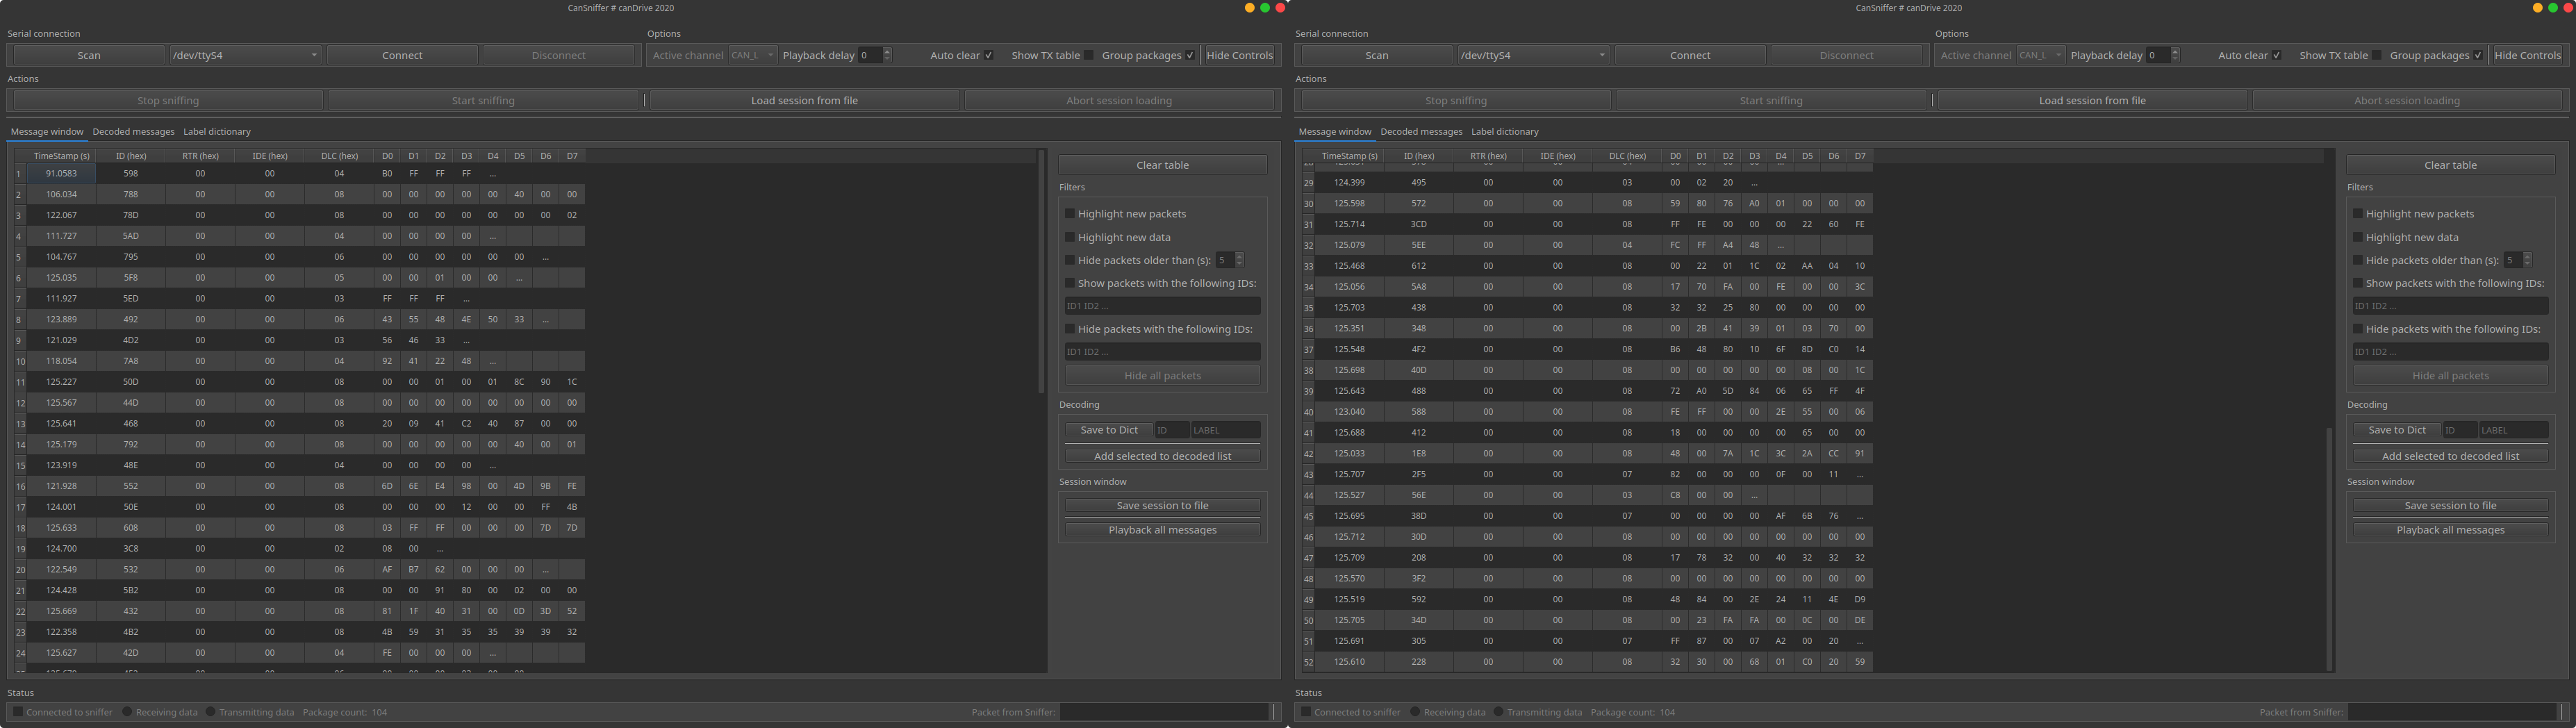
\includegraphics[width=0.8\textwidth]{test_obd.png}
  \caption{Missatges registrats durants les proves}
  \label{fig:test_obd}
  \end{figure}

Durant les següents proves es va detectar un nou problema, quan el dispositiu estava connectava al port \acro{obd-ii} i era alimentat externament al mateix temps, el vehicle detectava una anomalia, 
encara que no prou greu com per registrar un \acro{dtc}. En analitzar el sistema amb un osci\l.loscopi, es va observar que el pin TX de la ESP32 deixava passar un senyal residual abans 
d'inicialitzar el mòdul \acro{can}. Aquest senyal era convertit pel transceptor en un nivell de volatgte no vàlid que interferia amb el bus, en aquesta figura \ref{fig:Osciloscope} podem apreciar el senyal produit.

\begin{figure}
  \centering
  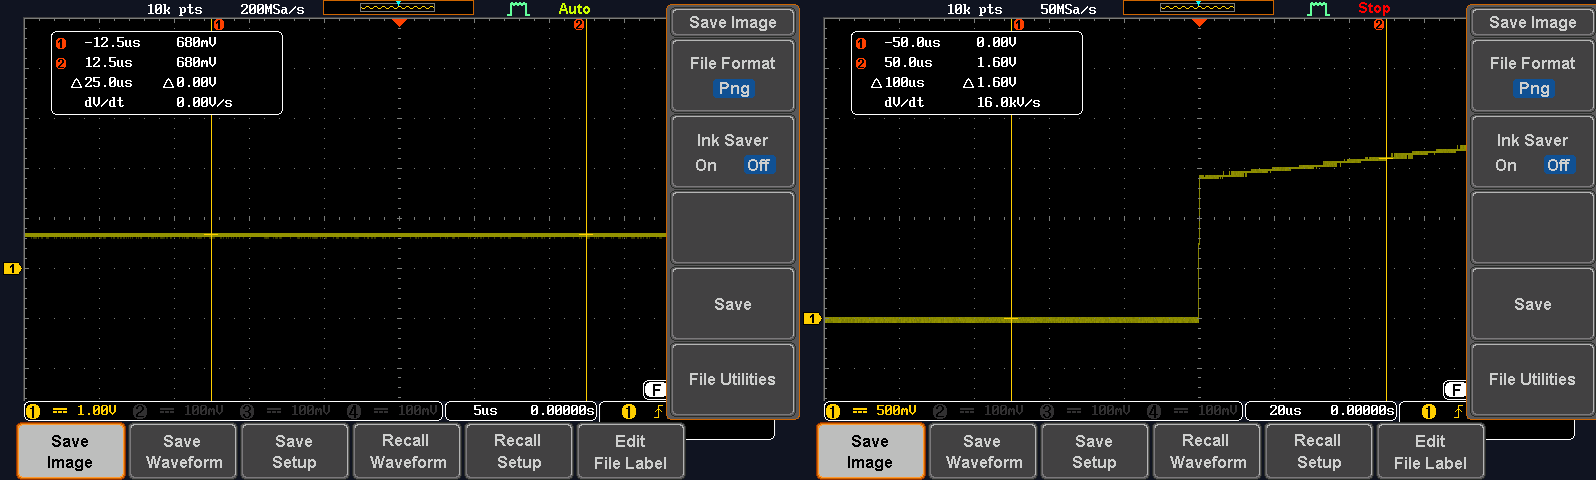
\includegraphics[width=0.8\textwidth]{Osciloscope.png}
  \caption{Mostra de l'socil·loscopi dles senyals de el pin de la ESP i el senyal resultant al transceptor}
  \label{fig:Osciloscope}
  \end{figure}

La solució va ser senzilla, es va assignar un pin \acro{gpio} diferent per al senyal TX, evitant així emissions prematures. Un cop aplicada aquesta correcció i realitzades les proves pertinents, 
es va confirmar que la comunicació amb el port \acro{obd-ii} funcionava de manera estable i fiable.

\section{Funcionalitat completa}

Per verificar el funcionament conjunt del sistema es va configurar un entorn de proves amb un portàtil que feia de servidor, allotjant tant el broker \acro{mqtt} com el servidor web, tots dos accessibles 
des de l'exterior mitjançant una \acro{ip} pública. Des d'un dispositiu mòbil es va accedir a la interfície web per visualitzar les dades en temps real, mentre es connectava el nostre dispositiu amb el 
transceptor provisional al vehicle.

El procés de prova seguia la seqüència operativa habitual: enviament de peticions \acro{pid} al bus del vehicle, identificació de les respostes i enviament d'aquestes dades al servidor mitjançant \acro{mqtt}. En 
connectar el dispositiu al vehicle, es va observar com les dades es reflectien correctament a la interfície web del client, coincidint amb els valors reals del vehicle i confirmant que el sistema 
complet funcionava com s'havia dissenyat.

\section{Placa i conversor DC-DC}

Un cop validades les funcionalitats bàsiques del sistema, es va procedir al muntatge físic del dispositiu en la placa \acro{pcb} dissenyada específicament per al projecte. Per obtenir la placa, 
es va utilitzar el servei de fresat de l'\acro{epsem} a partir dels arxius Gerber del disseny. Un cop fabricada, es va soldar tots els components que amb l'excepció del transceptor \acro{can} i el conversor DC-DC, 
van ser subministrats per l'\acro{epsem}. Aquest és l'aspecte del dipositiu final \ref{fig:device_photo}.

\begin{figure}
  \centering
  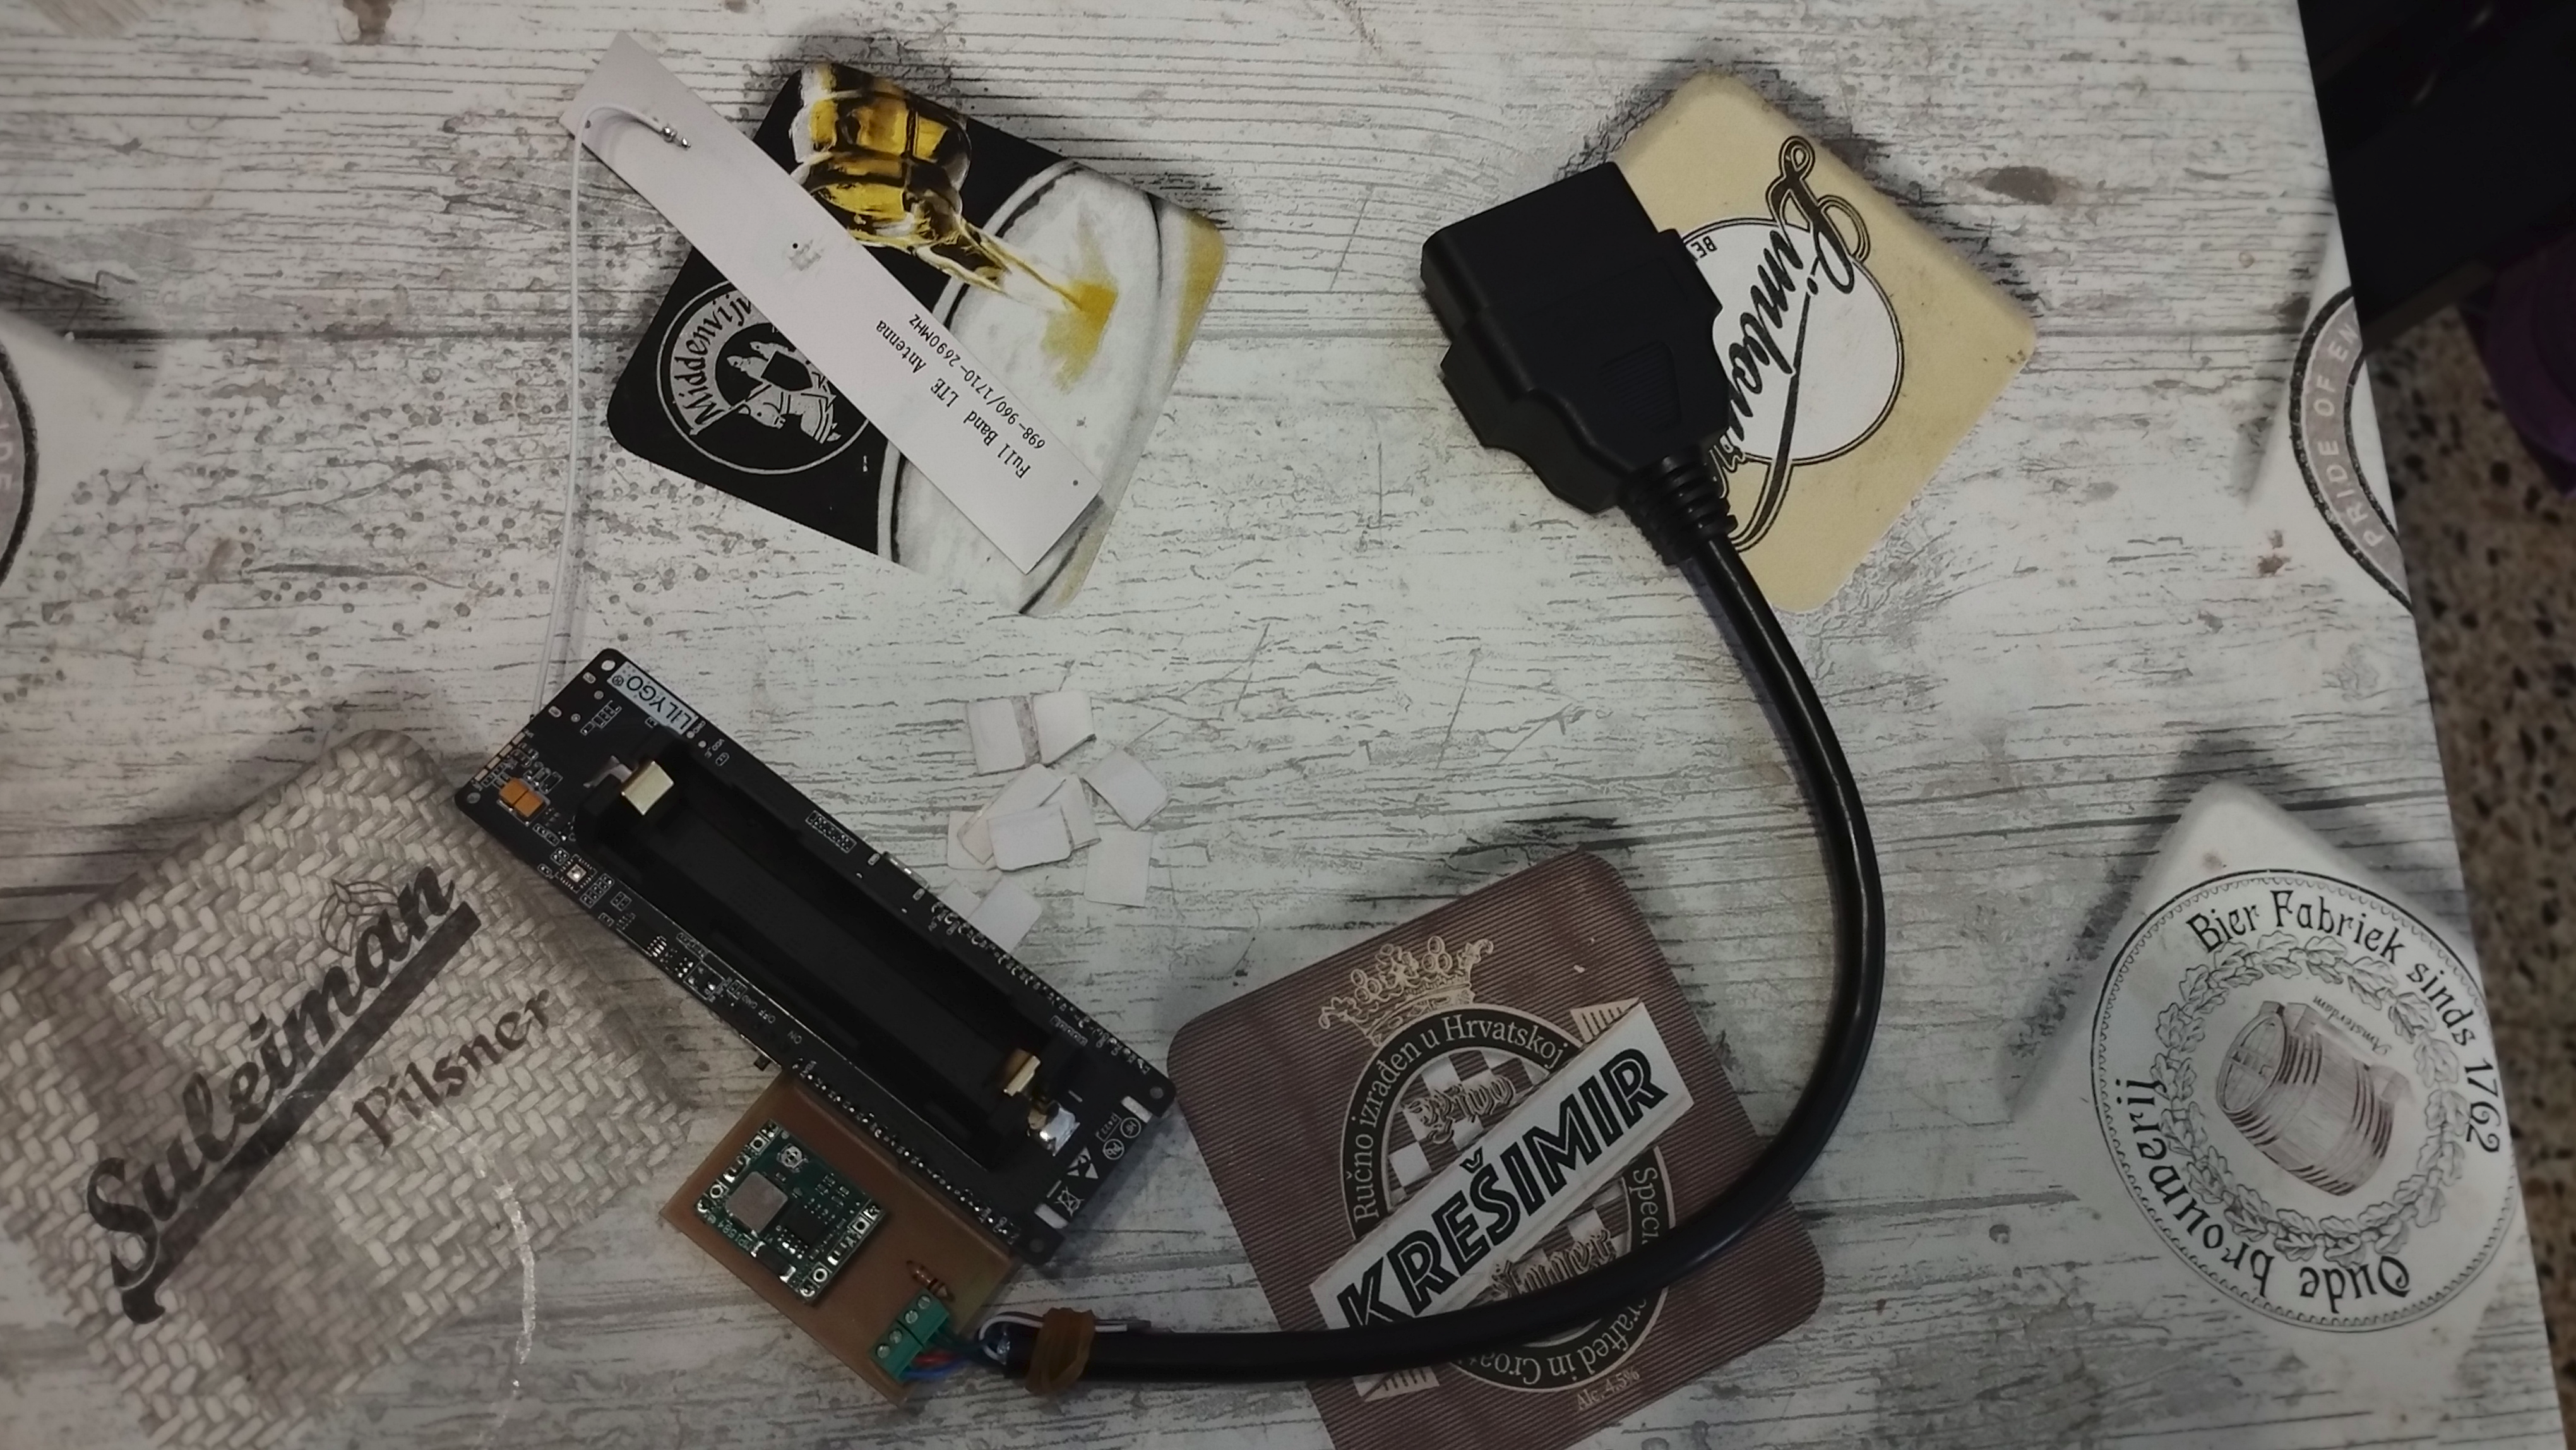
\includegraphics[width=0.8\textwidth]{device_photo.png}
  \caption{Dispositiu final}
  \label{fig:device_photo}
  \end{figure}


El procés de soldatge es va planificar per ser el més senzill possible, tot i que el transceptor en format \acro{smd} va presentar certa complexitat. Gràcies a les eines disponibles a l'\acro{epsem}, inclòs un 
microscopi, es va poder soldar tots els components sense incidències, malgrat la manca d'experiència prèvia en aquest tipus de muntatges.

Abans de la insta\l.lació definitiva al vehicle, es van realitzar proves individuals per verificar cada subsistema. Primer es va comprovar la comunicació \acro{can} sense alimentar la placa directament, 
amb resultats satisfactoris. Pel que fa al conversor DC-DC, es va verificar el seu funcionament abans de soldar-lo, i posteriorment es va testejar connectant la ESP32 a una font de 12V, observant-se 
un comportament correcte.

Finalment, en integrar tot el sistema al vehicle, es va confirmar el funcionament esperat de totes les parts. En aquesta figura \ref{fig:system_photo} es pot apreciar el dispositiu final connectat al vehicle mentre 
es proporciona la informació

\begin{figure}
  \centering
  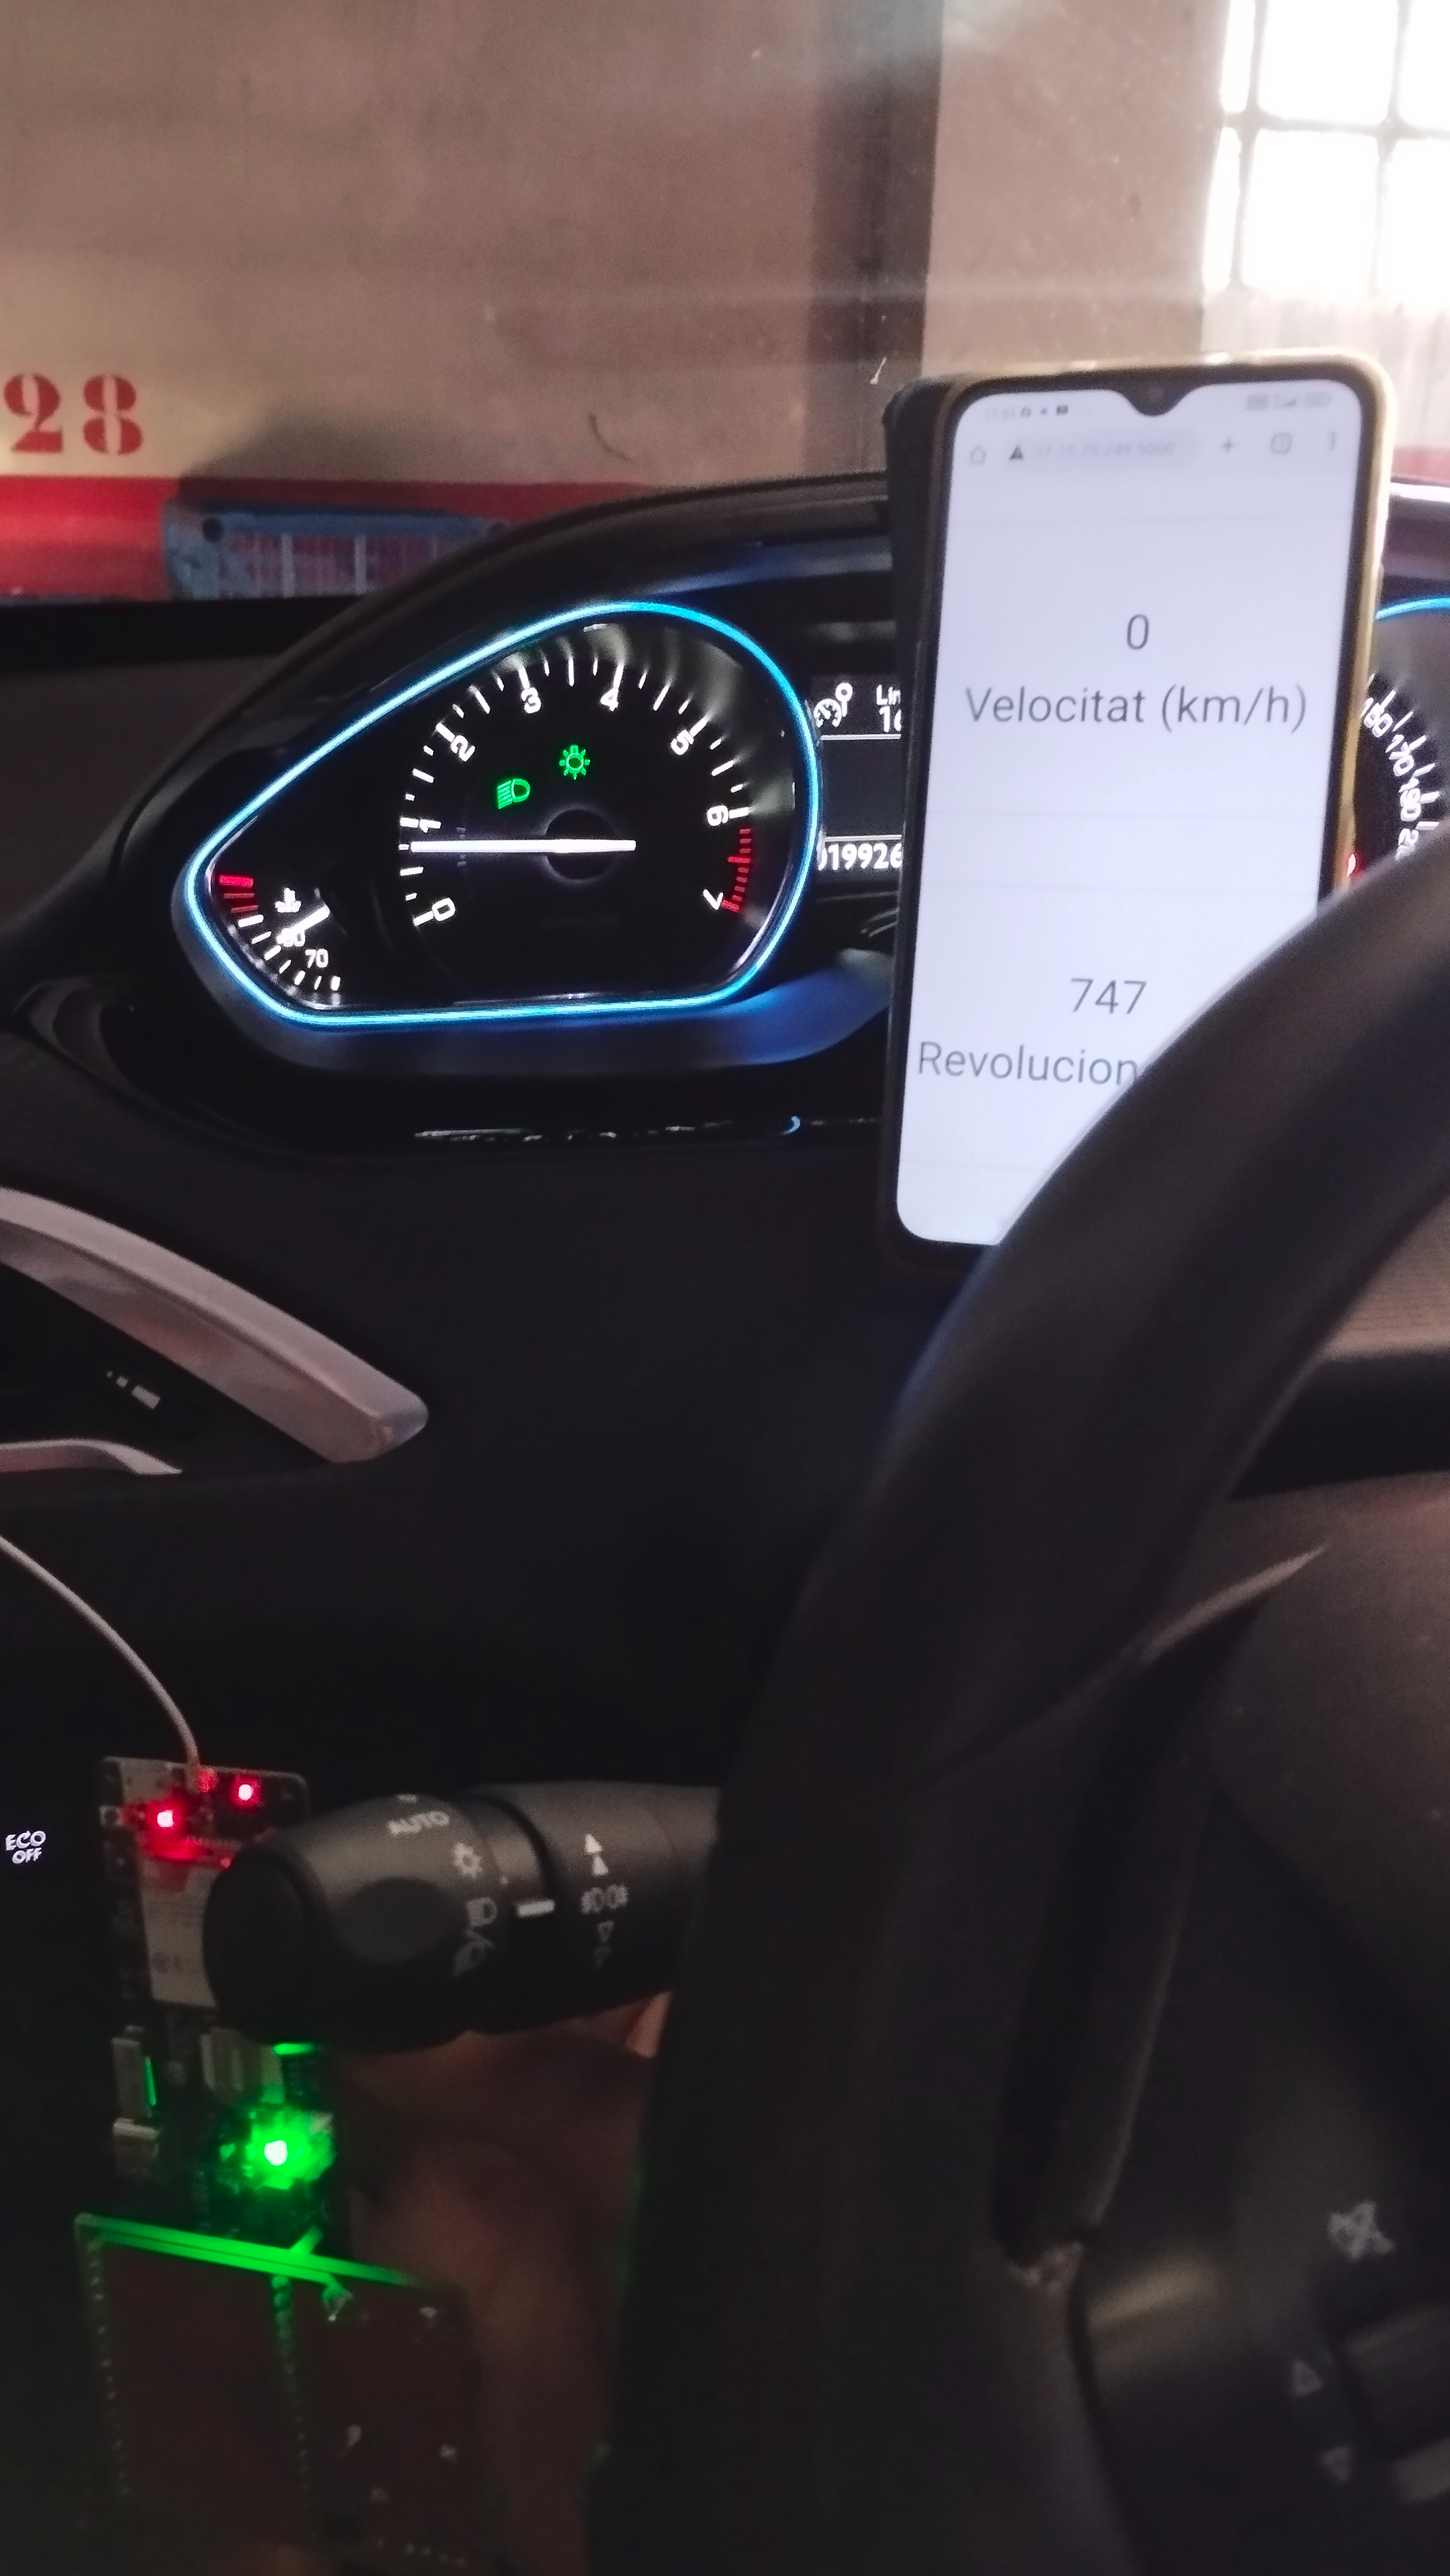
\includegraphics[width=0.8\textwidth]{system_photo.png}
  \caption{Dispositiu final connectat al vehicle en funcionament}
  \label{fig:system_photo}
  \end{figure}


\chapter{Conclusions}

En conclusió, s'han assolit els objectius principals plantejats en aquest treball. S'ha dut a terme una documentació exhaustiva sobre els sistemes de comunicació i diagnosi utilitzats en l'automoció, 
així com la implementació d'un dispositiu funcional capaç de monitorar remotament les dades del vehicle de manera eficient.

El protocol \acro{can}, base fonamental dels sistemes de comunicació dels vehicles moderns, ha estat analitzat en profunditat, incloent-hi les seves variants més rellevants i la seva integració dins 
l'estàndard \acro{obd-ii}. El mateix s'ha fet amb les funcionalitats i els detalls del protocol \acro{obd-ii}, incloent-hi explicacions sobre l'entorn real d'un vehicle.

Pel que fa al dispositiu desenvolupat, s'ha dissenyat i construït una placa de circuit amb tots els components necessaris per garantir una comunicació robusta tant amb el bus \acro{can} com amb 
la xarxa mòbil. El sistema és capaç de gestionar peticions \acro{pid} i rebre'n les respostes, a més de permetre la comunicació externa mitjançant \acro{mqtt}, tant en recepció com en transmissió per 
a la gestió del sistema, oferint una solució escalable per al monitoratge remot.

Aquest projecte constitueix, per tant, una base sòlida sobre la qual es pot desenvolupar un sistema de diagnosi més avançat. Tant el maquinari com el programari desenvolupats poden ser reutilitzats 
i ampliats amb mínimes modificacions per implementar funcionalitats més complexes.


\chapter{Ampliacions}

Durant el desenvolupament del projecte s'han assolit els objectius principals, aconseguint una base sòlida per a futures aplicacions relacionades amb la consulta de dades del vehicle. 
Tant la documentació generada com el codi font i el dispositiu dissenyat permeten ampliar fàcilment les funcionalitats actuals.

El sistema actual només interroga dos paràmetres bàsics: la velocitat i les revolucions del motor. L'objectiu era verificar que és possible obtenir dades en temps real del vehicle a 
través de l'\acro{obd-ii}. Tot i això, el sistema està plenament preparat per extendre aquesta funcionalitat. Només caldria afegir noves peticions \acro{pid} a la seqüència de consultes, gestionar 
les respostes corresponents i ampliar el sistema de recepció per identificar-les correctament. El codi ja disposa de funcions genèriques per a l'enviament de consultes \acro{pid} i l'emissió de
missatges \acro{mqtt}, de manera que els canvis requerits serien mínims.

En una fase inicial del projecte, es va considerar la possibilitat d'implementar un sistema d'enviament de missatges remots que permetessin accionar funcions del vehicle, com ara baixar 
les finestres. No obstant això, aquesta funcionalitat es va descartar degut als sistemes de seguretat del vehicle, que filtren aquest tipus de missatges cap a l'exterior. Malgrat això, 
el codi desenvolupat està preparat per rebre comunicacions mitjançant una subscripció \acro{mqtt}, la qual cosa obre la porta a futures implementacions. Les millores necessàries per dur a terme 
aquesta funcionalitat serien les següents:

\begin{enumerate}
    \item \textbf{Realització de proves en un altre vehicle}: Si es disposés d'accés a un vehicle sense filtres de seguretat per als missatges d'interès, es podrien registrar i descodificar aquests missatges.
    \item \textbf{Registre i processament de missatges}: Un cop identificats els missatges necessaris, es podria desenvolupar un sistema en què el client enviés una comanda \acro{mqtt} que, en ser rebuda pel dispositiu 
    (actualment només la mostra per pantalla), accionés una funció concreta del vehicle de manera remota.
    \item \textbf{Xifrat de les comunicacions}: Atès que el dispositiu pot actuar sobre el vehicle, és imprescindible garantir la seguretat de les comunicacions per evitar accions no autoritzades. Per això, es recomana 
    implementar TLS sobre \acro{mqtt} per xifrar les transmissions. Així mateix, seria convenient utilitzar HTTPS per a les peticions web i protegir les dades intercanviades amb el servidor.
\end{enumerate}

També es podrien desenvolupar millores a la part del client. Ja que aquest projecte posa l'èmfasi en la comunicació amb el vehicle, s'ha optat perquè la interfície sigui bàsica i funcional. 
Es podria desenvolupar un sistema d'usuaris on cada persona registrés el seu vehicle i accedís només a les dades associades. Això es gestionaria mitjançant una base de dades que emmagatzemés 
la informació recollida, permetent als usuaris consultar l'historial del vehicle.

Inicialment, es va planejar utilitzar el mòdul \acro{uart} per a la geolocalització, ja que aquests mòduls solen suportar comandes \acro{at} per a GPS. Tanmateix, després de realitzar proves i consultar \cite{lilygo_t76xx}, 
es va determinar que el mòdul utilitzat no suporta aquesta funcionalitat. Com que es tractava d'un aspecte secundari, es va descartar la implementació.

Un altre aspecte no abordat en profunditat és l'eficiència energètica del dispositiu. Encara que el consum de la ESP32 no és significatiu per a la bateria del vehicle, existixen modes de baix 
consum tant per al microcontrolador com pel transceptor \acro{can}. No obstant això, la seva implementació requereix una gestió acurada per assegurar que no es perdin missatges del bus \acro{can} o de \acro{mqtt} 
durant els períodes d'inactivitat.

\printbibliography

\end{document}

%%% Local Variables:
%%% mode: latex
%%% TeX-master: t
%%% LaTeX-biblatex-use-Biber: t
%%% End:
